% Martin Geidl, April 2004
% Theodor Borsche, April 2015
% Andrew Hamann, February 2018

\documentclass[a4paper,11pt,twoside,onecolumn]{book}
% Paper (210 x 297)
\usepackage[]{geometry}
\geometry{left=30mm,right=30mm,bindingoffset=0mm}
\geometry{bottom=30mm,footskip=13mm}
\geometry{top=30mm,headsep=8mm,headheight=5mm}

% Language
\usepackage[latin1]{inputenc} % Encoding of the input file
\usepackage[USenglish]{babel} % Language packages for hyphenation
\usepackage{ae} % Some additional fonts and symbols
\usepackage[stretch=3,shrink=3]{microtype} % Improves typography greatly
% Math
\usepackage{amstext,amssymb,amsbsy,amsmath}
\interdisplaylinepenalty=2500
\usepackage{mathtools} % Additional symbols and fixes
% Tables
\usepackage{booktabs}
\usepackage{floatrow}
\floatsetup[table]{capposition=top} % Ensure caption is above table
\usepackage{multirow}
% Miscellaneous
\usepackage{graphicx}
\usepackage[dvipsnames]{xcolor}
\usepackage{url}
\usepackage[ruled,vlined]{algorithm2e}
% Adjust float placement
\usepackage{float} % Additional float definitions and control
\renewcommand{\textfraction}{0.15} % Minimum amount of text on a page
\renewcommand{\topfraction}{0.85} % Maximum amount a figure at top may use
\renewcommand{\bottomfraction}{0.6} % Maximum amount a figure at bottom may use
\renewcommand{\floatpagefraction}{0.55} % Minimum amount a figure on its own page must use
\setcounter{totalnumber}{4} % Maximum number of figures per page
\setcounter{topnumber}{3} % Maximum number of figures at top
\setcounter{bottomnumber}{2} % Maximum number of figures at bottom
% Chapters and sections
\usepackage{titlesec}
\titleformat{\chapter}[display]{\filcenter}{\textit{\textbf{\huge \chaptertitlename\ \thechapter}}\vspace{7mm}}{0mm}{\Huge\textbf}
\titleformat{\section}[block]{\LARGE\bfseries}{\thesection}{0.5em}{}
\titleformat{\subsection}[block]{\Large\bfseries}{\thesubsection}{0.5em}{}
\titleformat{\subsubsection}[block]{\large\bfseries}{\thesubsection}{0.5em}{}
\titlespacing*{\chapter}{0mm}{17mm}{23mm}[0mm]

% Correct bad hyphenations
\hyphenation{op-tical net-works semi-conduc-tor}

\usepackage{lipsum}

\begin{document}
\frontmatter

% Title
\thispagestyle{empty}

\begin{center}

\vspace*{\fill}

\vspace*{\fill}

\textbf{\Huge Template for SAMA Reports}

\vspace*{\fill}

%

\textit{\large Student}

\textbf{\large Student Name}

\vspace{\baselineskip}

%

\textit{\large Supervisors}

{\large Assistant Uno}

{\large Dr.\ Post Doc}

\vspace*{\baselineskip}

%

\textit{\large Examiner}

{\large Prof.\ Dr.\ Gabriela Hug}

\vspace{\baselineskip}

%

\textit{\large Project Number}

{\large 1800}

\vspace{\baselineskip}

%

\textit{\large Report Date}

{\large February 8, 2018}

%

\vspace*{\fill}

\vspace*{\fill}

\textit{\large Power Systems Laboratory}

\vspace{0.5\baselineskip}

\textit{\large ETH Zurich}

\end{center}

%\noindent
\includegraphics[height=11mm]{logos/psl.pdf}
%\noindent\includegraphics[height=17mm]{logos/eth.pdf}

\chapter*{Abstract}
\lipsum[1-3]

\chapter*{Acknowledgements}
\lipsum[1-3]

\tableofcontents
\newpage

%\chapter*{List of Acronyms}
%\addcontentsline{toc}{chapter}{List of Acronyms}

%\chapter*{List of Symbols}
%\addcontentsline{toc}{chapter}{List of Symbols}

\mainmatter

\chapter{Introduction}
%\input{introduction}
\section{Background}

Background

Definition of flexibility

The challenges due to renewable penetration:

Traditional flexiblity from supply-side has limitations due to %Observations on market - increasing demands for flexibility due to renewable penetration

The increasing demand can be fulfilled in various means, including conventional methods like generation (gas turbine), tramsimission (grid extend), which normally requires vast investments on infrastructure. With the develop of technologies in ICT and batteries, new options are becoming increasingly feasbile %Observations on technology - reducing cost and increasing availability of technology

The push and pull from market demands and technology availability is leading the policy makers to review or even revise the regulatory framework which were established based on the  to allow non-discriminary participations of those new technologies. %Observation on regulation - regulatory changes, market redesign

Uncapping the potential

\section{Technologies: options for system flexibility provision}

\begin{itemize}
	\item supply-side flexibility
	\subitem Conventional power plant response
	\subitem Curtailment of variable renewable
	\item Energy Storage System (ESS)
	\subitem Battery Energy Storage System (BESS)
	\subitem Pumped Hydro Energy Storage (PHES)
	\subitem Compressed Air Energy Storage (CAES)
	\subitem Flywheel
	\item Demand Response (DR)
	\item Other
	\subitem Electric Vehicle to Grid (V2G)
	\subitem Electricity to Heat (E2H)
	\subitem Power to Gas (P2G) / Power to Hydrogen (P2H)
\end{itemize}

\section{Applications, benefits and business models}
\subsection{In liberalized market}

\subsubsection{Needs of different plyaers}

Player * Market * Application


\subsubsection{Energy Markets}


\subsubsection{Ancillary Service Markets}

\subsection{In vertically integrated market}


\section{Scope and research questions}

The target audience of this thesis is the management at Landis+Gyr on a high coporate level.

The ultimate goal is to provide references to support the audiences' strategic decision makings regarding flexibility management.

In order to achieve this, we conducted qualitative studies and developed quantitative models to identify: 1) the value of markets for flexiblity management

\begin{itemize}
	\item 
\end{itemize}

The goal of this thesis is to:

developed a robust modeling tool with moderate complexity so that it can not only provide results in current environment but can be also reused or easily revised to provide results in case of changes in the future.

based on the tool, make quantitative as well as quanlitative analysis to provide refer 

Purpose: providing references for strategic decision makings regarding flexibility management.

In order to make the analysis robust and reliable, we have built a techno-economic models which include the bottom-up dynamics of some key elements regarding the electricity markets and flexilibity technologies. 

However, it shall be noticed this thesis is not intended to serve for:

project developers to design a flexiblity system or make operating (including bidding) strategies of the system

policy makers to redesign the electricity market structure, rules or other policies

grid planners to understand the needs and options of flexibility in order to acheive system relability with lowest costs


Since the concept of flexiblity management is related to a great variety of technologies, applications and Landis+Gyr is positioning globally in various markets, the scope could be very broad. Nonetheless, in order to produce viable and reliable results with a solidily established techno-economic model, we have to make comprises. According to the relevance to Landis+Gyr's business, the scopes are defined as:

%\subsection{Scope of technologies}

%\subsection{Scope of applications}

%\subsection{Scope of benefits and business models}
The potential business model of Landis+Gyr is either to supply products to the customers to help them enable flexibility or to directly sell them flexible MWs as a service. In this case, we want to understand the value of each MW we enabled or sold. We assume Landis+Gyr will not directly partipate and trade in the power market, as it is going to place Landis+Gyr at the rival side of some customers in that market.

The value of flexibility will definitely vary according to the purpose, users' portfolio and operating strategies. 


%\subsection{Scope of markets}

\chapter{Sizing and Valuation of The Market for Flexibility Management: A Literature Review}
\chaptermark{Literature Reveiw}
\label{ch:LitRev}
\textit{This chapter reviews the existing literature on methodologies that are related to quantifying the market for flexibility management. It was found that our questions are not perfectly answered since existing research was geared to different stakeholders and perspectives. However, researchers have developed a number of validated methodologies which are of significant reference value for this study. We have mapped these studies and selected the ones we consider to be both effective and computationally tractable.}

\section{Stakeholders and their perspectives}

In this thesis, we aim at providing market analysis and valuations to support strategic decision making of technology vendors. There are similar works conducted by other firms and consultancies but their analysis along with the models are rarely made public \cite{Zucker2013}, because of concerns on commercial confidentiality. As a consequence, we referred to literature published either in academic journals or by regulated entities such as TSOs. Their motivations are often targeted at different audiences. We categorize the selected works into two groups with distinct perspectives, i.e. micro- and macro- system perspectives.

\subsubsection{Micro-perspective}

The first category refers to works that are concerned with the techno-economic performance of specific technologies in a given system/ market context as well as the value to one or few individual firms. This perspective is taken mainly to serve technical experts, flexibility project developers or investors in the context of a specific business or project.

In these works, valuation is usually a necessary component. The majority of these studies are made to propose novel technologies, control algorithms and bidding strategies etc. Valuation in these works is a metric to assess the technological feasibility and economic profitability in order to prove their concept. There are reports that exclusively focus on valuation in order to provide references on specific technologies or real projects \cite{Mokrian2006,Walawalkar2007,Sioshansi2009,Byrne2012,Berrada2016,Salles2017}.

Generally, this perspective shares the same interest as ours that is to maximize the financial benefits of market players. However, researchers tend to focus on project specifics. The associated complexity does not always add additional value to our more general purpose of assessing the total value of a market. Instead, due to limitations on computational tractability, it is challenging and time-consuming to apply these methodologies for dealing with large-scale data-sets. Most results are proof-of-concept for a methodology so cannot be used as direct inputs for our analysis. Besides, these models often have many implicit dependencies on market conditions so are less flexible while directly port into studies for a different market. Finally, most of these studies would assume their system size small enough that some market constraints such as liquidity can be ignored.

%Due to these reason, it was found that while the aggregation of different works could well cover our demands, there exists no individual work that perfectly solves our questions. In order to piece together their methodologies to build our own which is flexible to value different market and different technologies, we need to extract the principle rationales behind their models and grid rid of some unnecessary complexity, which is to be discussed in the next section.

\subsubsection{Macro-perspective}

Another perspective is taken by publications made for the interests of policymakers, market designers and grid planners. These studies stand on a macro-perspective and investigate the benefits or requirements of flexibility for power systems. They primarily pursue lowest system cost to ensure the adequate provision of flexibility. It is worthwhile to mention that these exercises done by grid planners, power system operators, and micro-grid operators are usually investigations on deferred infrastructure expenses \cite{Siano2014,HDREngineeringInc.2014,Gunter2016}, which are not within the core scope of this study.

The results derived from these models would be of less reference value for us, since we are primarily focusing on what can be retrieved by free players in power markets. Although outputs are often on a whole system level which look closer to estimations for the total market potential than results of studies with the micro-perspective, it shall be noted that there is seldom symmetry between remunerations obtained by players and contributions they make to the system due to imperfect market designs. For instance, in a paper that conducted valuations from both micro-perspective and macro-perspective, it was found that in several markets organized by independent system operators (ISOs) in the US the revenue obtained by flexibility suppliers was substantially less than the net benefit contributed to the system\cite{Denholm2013}.

Therefore, quantitative models developed in these reports will be seldom referred to by our study. Nonetheless, analysis and conclusions in these studies could help us better understand the needs of those policymakers, market designers and grid planners, which would have significant impacts on the landscape of flexibility management, so will be incorporated in our qualitative assessments. 

~\newline

It is worthwhile to emphasize that both perspectives have their own limitations. The models with micro-perspective are generally more precise but often case specific without a global view, while models with macro-perspective are very inclusive but unable to adequately represent all constraints and needs of each of the entities \cite{Zucker2013}. However, for each group of stakeholders, it is helpful to understand the rationale of the other group as well. Knowing the views of policymakers, market designers and grid planners will help players in power markets foresee the future movement of regulatory and market conditions so that they can make better decisions. On the other hand, policymakers shall consider the needs of market participants so that they can better encourage their participation by well-designed incentives.

As a consequence, there are researchers who conduct studies either with both perspectives in one piece of work such as \cite{Sioshansi2009,Denholm2009} or internalizing some decision factors from the other perspective into their own models, making the boundary less clearly demarcated. Nevertheless, in general we base our methodology primarily on works with micro-perspective due to the match of interests.



%Conventionally, their decision makings are supported primarily by commercial consulting firms who relied much on qualitative anlysis or quantitative data-anlytics. Even when sometimes it is possible that those firms have developed model with fundamental and physical approach, the model is always customized and not public 

%most of the researches are focusing one specific technology and one specific market, due to the nature of their target audiences. However, the managment iof a technology vendor will likely to be interested in various markets and various technologies. 

%The economics of flexibility solutions in power systems, especially electric energy storage (EES), is an active topic in research. It has drawn great attentions from the academics, investors and policy makers. 


% electricity storage are currently in the focus of research, by academics, utilities, potential investors as well as policy makers. The present document is the result of the analysis of more than 200 publications on that subject. It aims at presenting the “state of the art” regarding research on the economics of electricity storage. Three particular aspects are given attention to: the methodologies used, the profitability results obtained and the impact of regulation on storage economics.


%Policy maker: understanding the needs for flexibility, including the total amount and the mix, in order to provide guidance for regulated entities and market players

%Market designer: understanding the impacts of flexibility on current market design and find the most efficient market approach to enable them

%Grid planner (transmission and distribution system operator): understanding the value of flexibility that can help improve the reliability and stability of the grid with a lower cost

%Project developer of technical experts: proposing

%Depending on their role, different motivation and thus different methodologies. 

\section{Methodologies for quantifying the value of flexibility}
\sectionmark{Reveiw of Methodolgies}
Since our study is focused on income of flexibility management from power markets, it is necessary to incorporate power market modeling techniques. These models are found to be typically built in an optimization framework \cite{Zucker2013,GRUNEWALD2012449,VENTOSA2005897}. An optimization is applied to select the best combination of decision variables that maximizes the value of an objective function from some set of available alternatives, subject to some set of technical and economic constraints. In studies of our interests, the combination of decision variables is typically the dispatching plan of flexibility resources, and the objective function calculates the revenues or profits to remunerate owners. Thereby, the optimization is to estimate the maximum possible value obtained by players with a defined strategy and subject to constraints from markets and technologies. 

In terms of detailed implementation, these models can be classified into different approaches. Beyond briefly introducing these approaches, we analyze the rationale and proper use-case for each approach and then decide which ones to follow.

\subsection{Regarding market power: price taker versus price maker}
In economics, market power refers to the capability of a market participant to manipulate the price of an item to raise its own financial or strategic benefit. Market players with market power are often referred to as ``price makers" while those without market power are called ``price takers". It is worthwhile to mention that in perfectly competitive markets, market participants have no market power \cite{Mankiw2011}. 

In the business of flexibility management, players may be able to gain market power by deploying flexibility \cite{Zucker2013,Schill2011,He2012}.
This topic has attracted attention from researchers and many methodologies have been developed based on multi-optimization equilibrium modeling or making price a function of decisions. However, due to computational complexity, these methodologies are seldom used for valuation in real markets but more often for other use-cases, which are to be introduced in the reminder of this section.

\subsubsection{Single-optimization modeling vs. multi-optimization equilibrium modeling}
Single-optimization modeling is formulated with only one objective function, which represents the behavior of one entity without considering the  interactions with other actors. Single-optimization modeling is relatively easy to be formulated and solved with some established and powerful toolkit. Therefore, this modeling technique is adopted by most of studies on quantifying flexibility value, especially for those which were carried out based on real-world market data with a long span of time \cite{Walawalkar2007,Sioshansi2009,Byrne2012,Bradbury2014,McConnell2015,Berrada2016,Salles2017}

Multi-optimization equilibrium modeling considers the simultaneous benefit maximization of several entities to simulate the competition behaviors between them. Besides the lower level problem where each entity has their own strategy and objective, there is a upper level problem where the market clearing is simulated with interaction between entities under consideration. The upper level simulation usually requires advanced modeling techniques, e.g. agent-based modeling \cite{Yousefi2011,Dallinger2012,Zheng2014} and game theoretic approaches \cite{Schill2011,Gkatzikis2013,Lin2014,Kardakos2013}. The computational complexity will rise including the introduction of non-linearity, which will be discussed later in Section \ref{sec:formulating-solving}, and thus shall be only used for necessary cases. 

The main use of multi-optimization equilibrium modeling is to understand the market power and price maker effects. This could help market participants who have certain level of market power to strategically gain advantages in competition. For instance, Schill \textit{et al.} \cite{Schill2011} studied a case in Germany how the strategy on energy storage operation of major players as price makers would influence their own and other price takers' profits. Similar works have been performed for distributed generation (DG) aggregators \cite{Zhang2016}, DR aggregators \cite{HenriquezAuba2017} and more specialized EV aggregators \cite{Shafie-Khah2015}. Market designers may also need it to understand the impact of participation of new flexibility players and thus better organize their markets by eliminating possible market power \cite{Mohsenian-Rad2016,Vespermann2017,Huang2017}, or alternatively concentrating market power to regulated entities as proposed by \cite{He2012}.

Besides the computational complexity, performing multi-optimization equilibrium modeling requires extensive information such as the portfolio of each simulated entity. Therefore, it is more often that studies are based on a pseudo-market  \cite{Kardakos2013,Shafie-Khah2015,HenriquezAuba2017} than a real market \cite{Schill2011}.

%Therefore, equilibrium modeling is a helpful approach to understand the business rationales of price makers but is seldom used for estimating real market values considering computational tractability. 

%In our study, we are primarily focused on the value of market as whole rather than for individual players, so the competition between market players is less of our interest. An efficient market design is not within our core scope as well. Therefore, a single-optimization model should suffice our need, while a multi-optimization equilibrium model may be abused and not feasible to be applied for several real markets.

\subsubsection{Exogenous price vs. price as a function of decisions}

With a single-optimization approach, the upper level problem, i.e. market clearing, becomes an exogenous progress. The output of market clearing, price (and volume as well which is however rarely considered in literature), is a fixed input to the single-optimization model. In this way, the decision making entity is a price taker as its decision will not affect the price. 

An alternative way to internalize the price formation is to make the price a function of decision variables rather than being constant. However, such a method will make the optimization non-linear since the objective function is often the product of price and decision variables. The function has to retain some simplicity to be tractable. For example, Sioshansi \textit{et al.} \cite{Sioshansi2009,Sioshansi2010} used the simplest linear function for price and performed the optimization with a quadratic objective function. Due to this limitation, recent research works turn to the equilibrium model as introduced earlier to study situations with price makers. 

~\newline

Overall, although there is an abundance of literature studying price makers with flexibility, these methods are seldom applied for estimating real market values, which is however of most interest to us. Therefore, a pragmatic approach is to assume all participants are price takers. This assumption is definitely true when the market is perfectly competitive. Or according to the study based on actual market conditions in Germany \cite{Schill2011}, if energy storage capacities are allocated to generators reasonably (in line with their generation market share), total revenues from all players would remain almost unchanged whether dominant players act as price makers or price takers. Since we are primarily focused on the value of market as a whole rather than for each individual player, a price taker approach without considering the strategic interaction between players might suffice our needs, as is revealed by literature. Furthermore, while perfect competitive market may be an exorbitant assumption,  results based upon it do provide a decent benchmark reference.

\subsection{Predicting the price}
\label{sec:lit-price}
With the approach of single-optimization modeling using exogenous clearing, price is a crucial input to the optimization problem. It is of great importance how the value is obtained and how much foresight the decision makers have on price.

\subsubsection{Actual price signal vs. simulated price signal}

Some studies used real market data for valuation \cite{Walawalkar2007,Sioshansi2009,Byrne2012,Bradbury2014,McConnell2015,Berrada2016,Salles2017}. The merit of this approach is that they can provide the most accurate estimations although in a retrospective sense. The value will not depart significantly in short term since the power market was empirically found to stay relatively stable year over year, unless some exceptional events happened, e.g. the shale gas revolution in the US leading to drastic drop in electricity price around 2008 \cite{Brown2015,Salles2017}. However, those assumptions cannot remain valid in the long run. Moreover, increasing renewable penetration is accelerating the changes \cite{Woo2011,Gelabert2011,Mulder2013,Forrest2013,Wurzburg2013,Clo2015,Cludius2014}. 
For our study, this reveals the main drawback of using real market data being that it is not sufficient to provide long-term guidance, and the short-term view has to be renewed frequently. For research works that are concerned less on long-term scenarios such as the studies that just need to perform valuation for proof-of-concept, there is another issue. Directly using historical data as input eliminates the uncertainty of price together with associated risks.
%\cite{SaenzdeMiera2008} \cite{Tveten2013} \cite{McConnell2013}\cite{Gelabert2011}\cite{Clo2015} \cite{Woo2016}\cite{Cludius2014}\cite{He2013}\cite{Mulder2013}
Therefore, many studies developed auxiliary simulation models to generate price scenarios in complement to the main optimization program. For example, Grunewald \textit{et al.} \cite{Grunewald2012a} adopted a merit-order model to simulating wholesale electricity price setting behavior, thereby being able to generate price scenarios in the long run with changed generation mix as inputs for energy storage valuation. What is more commonly implemented by academic studies, as is mentioned, is simulating price uncertainties  in order to perform risk assessment. Seasonal autoregressive integrated moving average (SARIMA) is one of the most commonly used models to simulate the stochastic processes of electricity price \cite{Weron2014,Ziel2015,Mahmoudi2017,Alipour2017}. The SARIMA model is of order $(p,d,q)~\times~(P,D,Q)_s$. The terms $(p,d,q)$ represent orders of autoregression, differentiation and moving-average respectively while $(P,D,Q)_s$ correspond to orders of the seasonal part.
Alipour \textit{et al.} used a SARIMA $(2,0,2)~\times~(2,0,1)_s$ with seasonal part being AR (24,168) and MA (168)\footnote{The time step in this study is 1 hour. Therefore, 24 corresponds to the length of a day and 168 corresponds to the length of a week. The seasonal part is designed to capture the daily and weekly seasonality.} in this study where the profits of EV aggregators were assessed. Similarly, Mahmoudi \textit{et al.} \cite{Mahmoudi2017} implemented a SARIMA $(6,1,3)~\times~(1,0,0)_s$ with seasonal MA (168)\footnote{The time step is also 1 hour so 168 represents weekly seasonality.} to generate price scenarios for a stochastic program of DR aggregators. These stochastic models are estimated from historical data so cannot be applied solely to perform long-term forecast with changing generation mix.

In our study, both approaches using real market data and developing auxiliary price simulation models are applied, to estimate the market value under current market conditions and to understand the impact of possible changes of market conditions (increased RES penetration). For the price simulation model, the merit-order model and stochastic SARIMA model are synthesized, which will be discussed in detail in Chapter \ref{ch:methodology}.

It should be noted that among all the studies mentioned above, only one article \cite{Alipour2017} simulated the price for frequency control services in the short run using SARIMA model, while the others are exclusively for simulation of energy price. There is no literature found for long-term price trend of frequency control services. This can be explained by many reasons but most importantly it should be because the mechanism of price formation, the responsible party for procuring, as well as design specifications of frequency control services vary significantly among different market regimes and may change over time\footnote{More details and examples can be found in Section  \ref{sec:market-as}}. There are some works made on a macro-perspective to provide references for market designers and grid planner to anticipate future demand of frequency control services and propose improvements on frequency control market design \cite{GEEnergyConsulting2014,Scherer2016}. Nevertheless, the evolution of price level that is of more concern on a micro-perspective, was not discussed in the literature. Considering these limitations, we will only carry out quantitatively valuation for long-term scenarios for energy arbitrage, while for frequency control services we will quantify their market values under current market conditions together with some qualitative analysis.

\subsubsection{Perfect foresight vs. limited predictability}
\label{sec:perfect-forecast}
When historical data is directly used as input to the optimization, it contains an assumption that the decision maker has perfect foresight of the future price. This is the case of the studies mentioned previously \cite{Walawalkar2007,Sioshansi2009,Byrne2012,Bradbury2014,McConnell2015,Berrada2016,Salles2017}. The perfect foresight assumption leads to overestimation of the value of flexibility compared to what can be captured in reality \cite{Zucker2013}.

Stochastic price simulation, as introduced previously, is certainly a powerful way to resolve the issue. However, the stochastic approach adds complexity and requires more computation time, so deterministic approach is still favored in most cases. Therefore, some researchers ran sensitivity analysis to evaluate the level of overestimation caused by perfect foresight. Several authors applied methods such as reducing the forecast window \cite{Connolly2011} or using back-casting techniques, i.e. determine the future dispatch plan with historical data \cite{Sioshansi2009,Drury2011,Bathurst2003}. It was found that 60-90\% of the value with perfect foresight can be realized using primitive statistical price forecasting techniques. In reality, it is possible that players can apply some advanced forecasting techniques to make the value close to the ideal value obtained with perfect foresight. 

Therefore, the approach with perfect predictability is still useful to provide reference values indicating the upper bound. Sensitivity analysis might be necessary by reducing the predictability.

\subsection{Stacking technologies or applications}
\label{sec:lit-stacking}
Although many studies are carried out with one technology for one application, it is typically more complex in reality. Several technologies can be jointly organized and  dispatched to provide more than one type of services at the same time. These operating models may increase the profitability given the larger optimization space.

\subsubsection{Hybrid system}
A number of researchers studied the cases with hybrid systems, which are typically a combination between RES generation and one or several flexibility resources. While conventional research works were mainly focused on the large-scale wind and storage at one site \cite{Bathurst2003,Denholm2009}, increasing studies were carried out recently from the perspective of aggregators. Han \textit{et al.} \cite{Han2017} studied the optimal trading strategy of a VPP operator with distributed generations (wind power), energy storage and flexible load (load shifting). 
Calvillo \textit{et al.} \cite{Calvillo2016} investigated both panning and dispatching strategy of VPPs with photovoltaic (PV) systems, heat pumps (HP), batteries and demand response (load shifting) in Spanish wholesale energy market. Xu \textit{et al.} \cite{Xu2017} researched the optimal bidding strategy of aggregators with distributed generation, EVs and inflexible loads taking into account risk aversion. 

Referring to these studies, the most challenging issue to port this approach to our study is determining the optimal portfolio mix of the system. Among the articles mentioned above that are purely in micro-perspective, only the one authored by Calvillo \textit{et al.} \cite{Calvillo2016} studied the optimal planning by referring to methodology developed for microgrid (MG) operators \cite{Martin-Martinez2016}. For works focused primarily on operating and trading strategy, sizes are assigned arbitrarily to each technological sub-systems. For our study seeking to obtain the maximum value of the whole market, designing the optimal system mix for the whole system will be overwhelming and is a task of the grid planner, so it is not considered. Instead, we conduct separate investigation for each of the selected technologies.

\subsubsection{Multitasking}
In contrast to hybrid systems, a more common exercise of stacking is multitasking, i.e. offering several services at the same time. A typical combination of services is arbitrage plus frequency regulation. While some authors argue it is a necessary measure to make flexibility management solutions profitable \cite{Zucker2013,Megel2017}, we view it as a natural choice: most of the flexibility management systems have to participate in the wholesale energy markets in order to sell their bulk generation or fulfill their bulk demands; based on this prerequisite, while players plan to supply frequency control services that are normally more precious, they would naturally go for multitasking. Such type of multitasking are observed in studies on energy storage \cite{Byrne2012, Berrada2016,Megel2017}, EV2G \cite{Sortomme2012,Cho2015,Alipour2017,Peng2017} and DR \cite{Roos2014}.

Multitasking is performed and tested in our study.

\subsection{Formulating the problem}
\label{sec:formulating-solving}

\subsubsection{Deterministic modeling vs. stochastic modeling}
In our study, there lie many factors that are uncontrollable or not fully predictable. Besides the price in power markets that has been discussed already, there are still several key stochastic terms that are often encountered in studies related to flexibility management: 

\begin{itemize}
	\item The generation of variable RES such as wind and solar, and
	\item Frequency control signal from system operator, and
	\item End-users' behavior and thus availability of demand response.
\end{itemize}

Stochastic modeling would be helpful in cases where these terms are involved. Strictly, the objective function of an optimization with a stochastic approach is maximizing the expectation of value over different scenario and formulated as:  \cite{Zucker2013}:

\begin{equation*}
	\underset{x\in X}{max}\{ f(x) \equiv E[F(x(\omega),\omega) ] \}
\end{equation*}
 
where, $x \in \mathbb{R}^n$ is the vector of decision variables, $\omega \in  \Omega$ is the vector for the stochastic terms, and $F$ is the objective function. 

The articles authored by Qin \textit{et al.} \cite{Qin2012} and Xi \textit{et al.} \cite{Xi2014} are formulated in this way. It is worthwhile to mention that in the paper by Qin \textit{et al.} \cite{Qin2012}, only the uncertainty of price was considered while the frequency control signals are treated as deterministic. 

Nonetheless, most of the studies on flexibility management with stochastic approach are virtually scenario-based deterministic programming. Their objective function is to maximize the objective value for each scenario and formulated as:

\begin{equation*}
\underset{x\in X}{max}\{ f(x) \equiv F(x(\omega),\omega)\}
\end{equation*}

where, $x \in \mathbb{R}^n$ is the vector of decision variables, $\omega \in  \Omega$ is the vector for the stochastic terms, and $F$ is the objective function. 

Such a problem formulation is used in \cite{Zhang2016,Alipour2017,Mahmoudi2017,Xu2017,Han2017,Calvillo2016,Mahmoudi2014}. More specifically, Zhang \textit{et al.} \cite{Zhang2016} considered the uncertain outputs of DG. Mahmoudi \textit{et al.} \cite{Mahmoudi2017} use a random Boolean indicator to represent the participation of DR customers. Xu \textit{et al.} \cite{Xu2017} studies a system with DG, DR and EV but particularly focused on the EV uncertainty with the arrival/departure time, driving distance sampled randomly from historical probability distributions. Uncertainty of frequency control signals was modeled by Alipour \textit{et al.} \cite{Alipour2017} where the randomness of price and EV availability are considered as well. 

In works where multiple stochastic terms are considered, a multi-stage scenario-based optimization was applied \cite{Alipour2017,Han2017}.

Nonetheless, stochastic approach is not a must \cite{Zucker2013}. Using the deterministic approach for the most likely scenario is sufficient to provide a decent reference value compared to the result from stochastic programming, as was illustrated by \cite{Calvillo2016}. The most important outcome obtained with stochastic approach in addition to results using deterministic approach is risk control. 

In our study, we apply the deterministic approach most of the time. Scenario-based optimization is performed only in cases where the stochastic price simulation is involved.

\subsubsection{Linear programming vs. non-linear programming}

Non-linearity is not favored in optimization which would significantly reduce the computational tractability and is likely to make the optimization non-convex.

In the studies we have reviewed, non-linearity may be introduced in various ways, including:
\begin{itemize}
	\item The upper level market clearing problem in the multi-optimization equilibrium models is usually not linear. \cite{He2012,Mohsenian-Rad2016,HenriquezAuba2017,Vespermann2017,Huang2017} 
	\item Non-linear relations may exist between cost and decision variables \cite{Mahmoudi2017}.
\end{itemize}

Typically, researchers seek measures such as the primal-dual approach to convert the non-linear programming to be mixed integer linear programming \cite{Zhang2016,Storage2015,HenriquezAuba2017,Mohsenian-Rad2016} or to approximate the non-linear objective function using a piece-wise linear function \cite{Mahmoudi2017}.

In our study, we avoid to include non-linearity in our optimization. Any relations that may cause non-linearity such as the price formation are taken out of the optimization and coped with separately.

\section{Summary}

%\subsection{Determining the value of flexibility for specific cases/ projects}
%Firstly, the most abundance of articles were related to accessing the techno-economic performance of specific technologies, in given system system/ market contexts (typical one technology in one context). This corresponds to the view of a project developer or technical experts. In these researches, they would propose innovated technologies, or novel design/ operating strategies and validate by valuation. 



%\subsection{Determining the demands for flexibility at a system level}




%\subsubsection{Predictability and stochastic modeling}





%\section{Summary of existing works and the implications on our study}

%As we have seen, there is a great abundance 
%Since our perspective does not perfectly in most academic articles, there does exist a perfect valuation framework that can be directly port into our study. Therefore, we mapped a number of research papers with different approach and selected the proper ones considering  both effectiveness and computational tractability. 

%Combining trivial makes it nontrivial




%As is clearly revealed by the literuare review, there exist abused research articles generally on this topics of flexibility management. However, there exist very few academic works that serves the needs of our target audiences who are the management of technology vendors. The deviationsof interests result in gaps that make it difficult to directly use the existing works. These gaps include:

%\begin{itemize}
	%\item Most of the researches are based on one specific technology and one specific market, as usually a utility company or a grid planner is operating in one market regimes and a technical professional is focusing on one technology.  However, our target audiences are likely to be interested in various markets and technologies.
	%\item Scope
	%\item Mothed - proof of concept
%\end{itemize}


\chapter{Power Market Framework and Proposed Business Model for Flexibility Management in Selected Segments and Geographies}
\label{ch:market}
\section{Power market framework}

\subsection{PJM}

\subsection{Germany}
\label{market:germany}

\subsection{Balancing Energy Market}

%Market participants in Germany are organised into balancing groups, known as Bilanzkreise (BK). BK can range from individual large generators to aggregations of smaller renewable generations, to a Stadwerke representing large portions of aggregated demand.

%Every balancing group operator is responsible for following a planned schedule with a 15-minute resolution. Deviations from the planned schedule are balanced physically by the TSOs and settled financially with the BK. There is a legal obligation on Bilanzkreise to balance their positions to the best of their ability.

Prices for balacning energy are unified across TSOs and determined according to the  balancing energy price settlement system (BK6-12-024) developed by Federal Network Agency (FNA) as of 01/12/2012.

\begin{equation}
reBAP = \frac{\sum net imbalance energy cost}{\sum net imbalance energy volume}
\end{equation}

%\chapter{Methodology for Quantitative Valuation of Flexibility Management Markets}
\textit{This chapter presents the methodology for quantifying the value of flexibility managment markets. A modular approach is adopted to overcome the complexity from multi-dimensional market-technology contexts. Firstly, the modules are introduced, being categorized into market- and technology- based groups. Then we will explain how these modules are to be organized within a optimization.}

\section{Modular approach to build valuation models}
In this thesis, a list of different markets and two different technologies are being studied. This results in a significate number of cases of environment. It is not possible to generalize the model for these cases due to multi-dimensional structural differences. On the other hand, building a model for each case will lead to redudancy and make the model less usable and harder to maintain. Therefore, we adopt a modular approach where the dynamics of markets (or technologies) are generalized and varable in market-based (or technology-based) modules. The modular approach does not reduce the complexity of the problem, but renders the model more structurally organized.

\begin{table}
	\label{tb:modules}
	\begin{center}
		\begin{tabular}{|m{1.5cm}| m{2.75 cm} | m{4 cm} | m{4cm} |}
			\hline
			\textbf{Section} &\textbf{Module name} & \textbf{Input} & \textbf{Output} %& \textbf{Parameters}
			\\[0.5ex]
			\hline \hline
			\multicolumn{4}{|c|}{Market-based modules }\\
			\hline
			4.2.1&Revenue module & Price signals (Determinate part), Frequency control singals, Sets of targeted marketplaces & Matrix of coefficients for revenue calculation %& None 
			\\
			\hline
			4.2.2&Risk module & Price signals (Distribution of stochastic part), Frequency control singals, Sets of targeted marketplaces& Matrix of coefficients for calucating Conditional Value-at-Risk %& Confidence level 
			\\
			\hline
			4.2.3&Market simulation module & Generation by fuel type, consumption and its elasticity& Price and volume signals% & The parameters were  obtained by regression with historical data 
			\\
			\hline
			4.2.4&Market constraints & Volume signals & Constraints for optimization %& Market rules 
			\\
			\hline
			\hline
			\multicolumn{4}{|c|}{Technology-based modules }\\
			\hline
			4.3.1&Cost module & Investment cost, Designed life time, Operating life time, System state & Matrix of coefficients for cost calculation %& None
			\\
			\hline
			4.3.2&Technology simulation module & Efficiencies of charging, discharging and storing; Capacity; Energy-to-power ration& Matrix of coefficients to determine system states %& 3
			\\
			\hline
			4.3.3&Technology constraints & Historical data (Generation by fule type, consumption, market price and volume)& Price and volume signals %& 3 
			\\
			\hline
		\end{tabular}
	\end{center}
	\caption{List of modules}
\end{table}

\begin{figure}[h!]
	\label{fig:model-flow}
	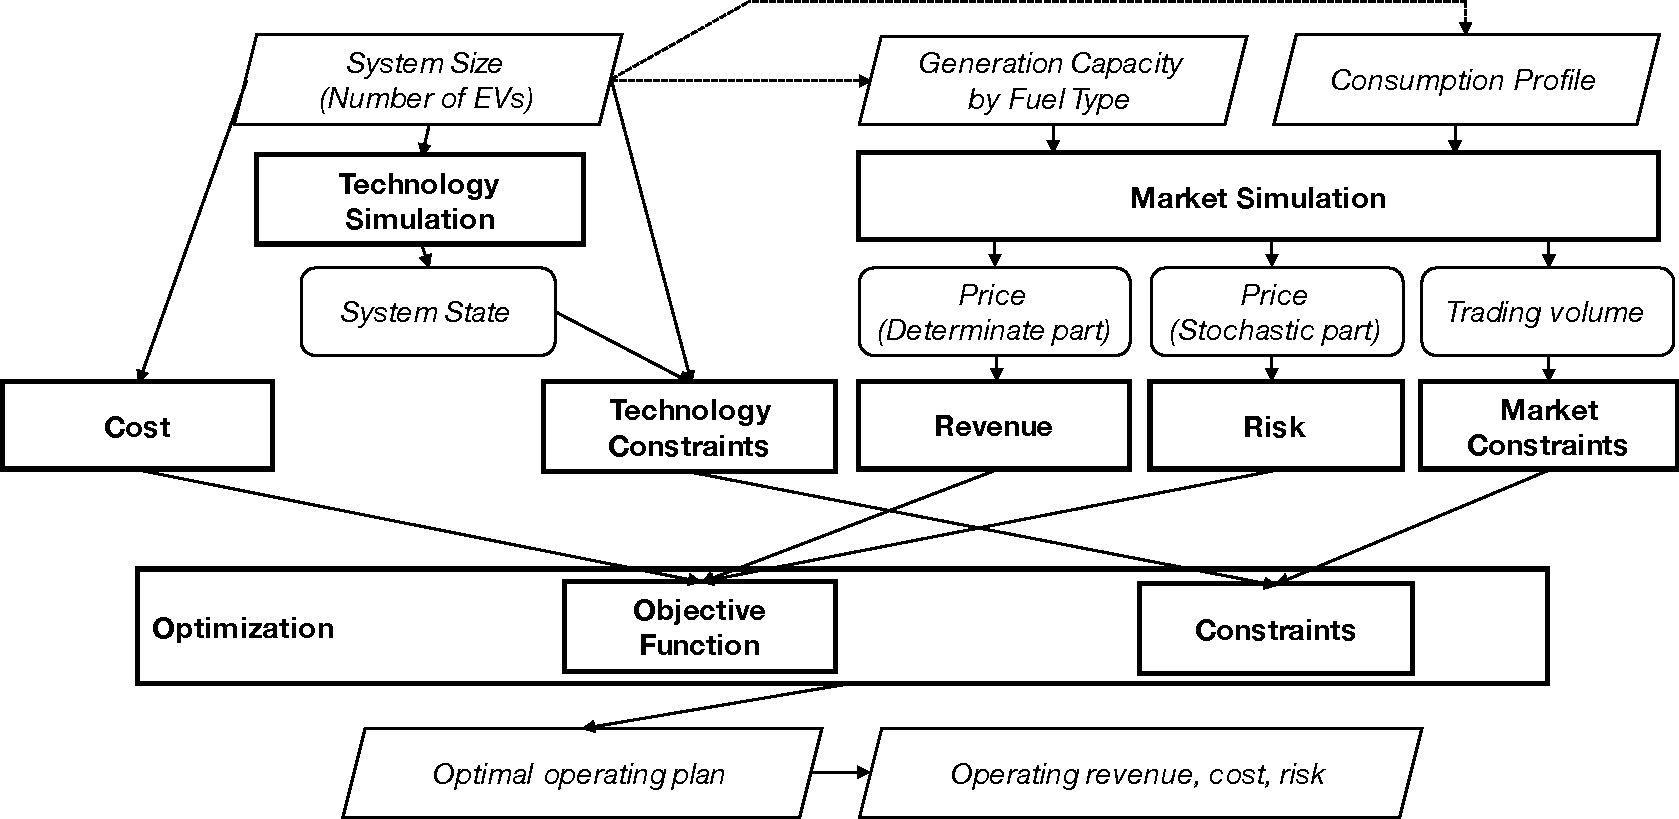
\includegraphics[scale=0.4]{Figures/ModelFlow.pdf}
	\caption{Flow chart of the techno-economic model}\
\end{figure}

Table \ref{tb:modules} offers an overview of all the modules and their inputs and outputs. The working flow of the model is illustrated by Figure \ref{fig:model-flow}.

With this model, we can evaluate the profitability and risk associated with a certain scale of flexibility management system in the power market and thus estimate the value of flexibility management market. Furthermore, we can assess the impact of driving factors including renewable penetration, cost reduction, and the possible diminishing return with increasing flexibility.

\section{Market-based modules}

\subsection{Revenue module}

In this study, we only consider explicit revenues from power markets. At each time step ($t$), the revenue ($\text{REV}_t$) is calculate as the amount of energy ($e_t$, in MWh) offered in each energy market segment ($i$), and/or amount of reserve ($r_t$, in MW) offered in each reserve market segment ($j$), multiplied by their corresponding prices ($\pi_t$, in \$/MWh or \$/MW). In reserve market, there are additional revenues from energy provision while the committed capacities are activated. The amount of energy delivered in reserve market is determined as a proportion of the committed reserve using a term of ratio ($\delta_t$, in MWh/MW). The total revenue within a given period of time ($T$) and a set of selected energy markets ($I$) and a set of  selected reserve markets ($J$), can be then computed as:

\begin{equation}
\label{eq:module-revenue}
\text{REV}=  \sum_{t}^{t \in T} \text{REV}_t = \sum_{t}^{t \in T} \left( \sum_{i}^{i \in I}  \pi_t^{e,i} (e_t^{d,i} - e_t^{c,i})  + \sum_{j}^{j \in J} (\pi_t^{e,j} \delta_t^{j} + \pi_t^{r,j}) r_t^j \right)
\end{equation}

where, $d$ and $c$ in the superscripts denote "discharge" (to release energy from flexibility resources to grids) and "charge" (to intake energy from girds to flexibility resources) respectively.  $e_t^{d,i}$, $e_t^{c,i}$, $r_t^{j}$, are endogenous variables of the whole model and decision variables of the optimization, which represent the operation plan of the flexibility resource in power markets.

$I$ and $J$ are determined according to the business case being studied. For example, we can set $I = \{Day~ahead\}$ and $J=\emptyset$ in order to the value of making arbitrage in day-ahead energy market. 

If there are multiple elements in $I \cup J$, it means the flexibility resource can be reallocated to make offers to different market segments, i.e. performing multitasking. These cases need to be carefully managed to comply with actual market rules. Detailed treatments regarding multitasking are illustrated in section \ref{sec:special}.

The ratios $\delta_t$ are computed based on the real control signal when data is available, or otherwise using system average ratios between total activated energy ($\hat{e}_t^{r,j}$) and the total reserve ($\hat{e}_t^{r,j}$) at each time step.

%\begin{equation*}
%\delta_t^j = \frac{\hat{e}_t^{r,j}}{\hat{r}_t^j}
%\end{equation*}

Price signals, $\pi_t^{e,i}$, $\pi_t^{r,j}$ and $\pi_t^{e,j}$, are inputs for the revenue module and may be retrieved either directly from historical data or from the outputs of market simulation module described in Section \ref{sec:market-simulation}.

We re-formulate Equation \eqref{eq:module-revenue} in form as:

\begin{equation*}
\text{REV} = \textit{\textbf{f}}~X
\end{equation*}

where $X$ is the vector for all desicion variables. For certain sets of market segments $I$ and $J$, $X$ can be derived using Equations \eqref{eq:decision-variable-1} - \eqref{eq:decision-variable-end} with $i \in I$ and $j \in J$.
\begin{equation}
\label{eq:decision-variable-1}
X =
\begin{bmatrix}
E^d \\ E^c \\ R
\end{bmatrix}
\end{equation}

\begin{equation}
E^d =
\begin{bmatrix}
E^{d,I(1)} \\ \vdots \\ E^{d,i} \\ \vdots \\ E^{d,I(|I|)}
\end{bmatrix} \\
E^{d,i} = 
\begin{bmatrix}
e_1^{d,i}\\e_2^{d,i}\\\vdots\\e_T^{d,i}
\end{bmatrix}
\end{equation}

\begin{equation}
E^c =
\begin{bmatrix}
E^{c,I(1)} \\ \vdots \\ E^{c,i} \\ \vdots\\ E^{c,I(|I|)}
\end{bmatrix} \\
E^{c,i} = 
\begin{bmatrix}
e_1^{c,i}\\e_2^{c,i}\\\vdots\\e_T^{c,i}
\end{bmatrix}
\end{equation}

\begin{equation}
\label{eq:decision-variable-end}
R =
\begin{bmatrix}
R^{J(1)} \\ \vdots \\R^{j} \\ \vdots \\ R^{J(|J|)}
\end{bmatrix} ~~~\\
R^{j} = 
\begin{bmatrix}
r_1^{j}\\r_2^{j}\\\vdots\\r_T^{j}
\end{bmatrix}
\end{equation}

Function $\textbf{f}$ can be obtained analogously using Eqution \eqref{eq:decision-f-revenue-1} $\sim$ \eqref{eq:decision-f-revenue-end} with $i \in I$ and $j \in J$.
\begin{equation}
\label{eq:decision-f-revenue-1}
\textit{\textbf{f}} =
\begin{bmatrix}
\Pi^{e,I}~|~&-\Pi^{e,I}~|~&\Pi^{e,J} \Delta^J + \Pi^{r,J}
\end{bmatrix}
\end{equation}

\begin{equation}
\Pi^{e, I} =
\begin{bmatrix}
\Pi^{e,I(1)}~|~&\dots~|~&\Pi^{e,I(|I|)}
\end{bmatrix} ~~~\\
\Pi^{e,i} = 
\begin{bmatrix}
\pi_1^{e,i}~\pi_2^{e,i}~\dots~\pi_T^{e,i}
\end{bmatrix}
\end{equation}

\begin{equation}
\Pi^{e,J} =
\begin{bmatrix}
\Pi^{e,J(1)}~|~&\dots~|~&\Pi^{e,J(|J|)}
\end{bmatrix} ~~~\\
\Pi^{e,j} = 
\begin{bmatrix}
\pi_1^{e,j}~\pi_2^{e,j}~\dots~\pi_T^{e,j}
\end{bmatrix}
\end{equation}

\begin{equation}
\Pi^{r,J} =
\begin{bmatrix}
\Pi^{r,J(1)}~|~&\dots~|~&\Pi^{r,J(|J|)}
\end{bmatrix} ~~~\\
\Pi^{r,j} = 
\begin{bmatrix}
\pi_1^{r,j}~\pi_2^{r,j}~\dots~\pi_T^{r,j}
\end{bmatrix}
\end{equation}

\begin{equation}
\label{eq:decision-f-revenue-end}
\Delta^J = diag (
\delta_1^{J(1)}, \dots , \delta_T^{J(1)}, \dots, \delta_1^{J(|J|)}, \dots, \delta_T^{J(|J|)})
\end{equation}

\subsection{Risk module}
In accordance with the revenue calculation, we consider the uncertain movement of price as the primary source of risk. Referring to similar works that performed risk management for flexibility sources, e.g. EV2G \cite{Alipour2017} and DER \cite{Han2017}, as well as for conventional energy trading companies \cite{Mohammadi-Ivatloo2013}, we developed a simple measure for risk control, by using the conditional value-at-risk (CVaR).

The CVaR (also named expected shortfall) as an extension of value-at-risk (VaR) can be defined as the difference between the expected profit and the average of potential profit values which are less than VaR \cite{Rockafellar2000}, shown as:

\begin{equation}
\label{eq:CVaR}
CVaR_\alpha (X) = \int_{\alpha}^{1} VaR_s(X) ds
\end{equation}

where $\alpha$ is the confidence level, and $X$ is the underlying (the price of energy/ reserve in our study). The VaR, as the negative of $\alpha$-quantile, can be computed as:

\begin{equation}
\label{VaR}
VaR_\alpha(X) = inf \{x \in \mathbb{R}~|~ P(X+x<0)\leq 1-\alpha\}
\end{equation}

Specially, in case the underlying variable subject to normal distribution, i.e. $X \sim \mathcal{N}(\mu,\,\sigma^{2})\,$, we can derive the CVaR as:

\begin{equation}
CVaR_\alpha(X) = \mu - \sigma \frac{\phi(\Phi^{-1}(\alpha))}{1-\alpha}
\end{equation}
%http://blog.smaga.ch/expected-shortfall-closed-form-for-normal-distribution/
where, $\Phi(\cdot)$ is cumulative distribution function and $\phi(\cdot)$ is the probability density function of normal distribution.

Alternatively, if the uncertainties are dealt with in a discrete manner, the CVaR can be calculated as\cite{Rockafellar2000}:

\begin{equation}
CVaR_\alpha (X) = \underset{\zeta}{max}\left( \zeta - \frac{1}{1-\alpha} \sum_{s} P(X,s) (\zeta - f(X,s))\right)
\end{equation}
where, $P(X,s)$ is the probability distribution function of $X$ in the scenario $s$ and $f(X,s)$ is the profit function in the scenario $s$. $\zeta$ is an auxiliary variable constrained by

\begin{equation*}
\zeta - f(X,s) \leq \zeta_s
\end{equation*}
\begin{equation*}
\zeta_s \geq 0
\end{equation*}

In our study, price terms $\tilde{\pi}$ are assumed to comprise a determinate part $\pi$ and an independent stochastic deviation $\epsilon$:
\begin{equation}
\label{eq:price-error}
\tilde{\pi_t}= \pi_t + \epsilon_t
\end{equation}

Since the stochastic terms $\epsilon$ are assumed to be uncorrelated to each other, the CVaR of our portfolio that is built by  $X^T = [E^d~|~E^c~|~R]$
in Equation \eqref{eq:decision-variable-1} can be aggregated as:

\begin{equation}
\begin{aligned}
CVaR =\sum_{t}^{t \in T} \{&\\
&\sum_{i}^{i \in I}  CVaR(\tilde{\pi_t}^{e,i}) (e_t^{d,i} - e_t^{c,i})  \\
&+ \sum_{j}^{j \in J} \left(CVaR(\tilde{\pi_t}^{e,j}) \delta_t^{j} + CVaR(\tilde{\pi_t}^{r,j})\right) r_t^j \\
&\}
\end{aligned}
\end{equation}

Analogous to the formation in preceding section, the risk module is also formulated in vector and matrix form.

\begin{equation*}
CVaR= \textit{\textbf{f}}
\begin{bmatrix}
E^d \\ E^c \\ R
\end{bmatrix}
\end{equation*}

where \textit{\textbf{f}} is calculated as:

\begin{equation}
\textit{\textbf{f}} =
\begin{bmatrix}
CVaR(\Pi^{e,I})\\-CVaR(\Pi^{e,I})\\CVaR(\Pi^{e,J}) \Delta^J + CVaR(\Pi^{r,J})
\end{bmatrix}^T
\end{equation}

\subsection{Market simulation module}
\label{sec:market-simulation}
As has been illustrated in the literature review (Chapter \ref{ch:LitRev}), valuation of flexibility with a dynamic market condition is still a challenging task. While investment decisions are extensively concerned with long-term trends, profitability of arbitrage sensitively depends on short-term price movement in high resolution. This is distinguishing from conventional electricity generators for whom a long-term forecast with coarse resolution is sufficient, and visual arbitrageurs who have almost no investments on infrastructures and may perform decision-makings with a short-term perspective. A holistic approach combining these researches were taken sometimes \cite{Rastler2010}\cite{Eyer2010} but may easily bring in unnecessary complexity and lead to an overwhelming demand of resources, which are not essential for our study.

Therefore, in this thesis, we customized a market model based on existing researches by re-focusing on factors that are most relevant to our research questions, and simplifying many other aspects of the power system and markets. Our market model is generally a statistic model built on observations of historical data, but a physical sub-model is incorporated as well to study the impacts of some relevant variables whose features are not well captured by empirical observations.

The approach for market simulation differentiates between energy markets and reserve markets. 

The energy markets are usually matured and with abundant degree of competition, so that we can employ an idealistic market model where the price formation is governed by the short run marginal costs (SRMCs) \cite{Grunewald2012} \cite{Grunewald2012a}. This allows us to leverage a merit-order model to simulate the price levels, which are widely adopted as is summarized in Chapter \ref{ch:LitRev}. 

The design of reserve markets, on the contrary, is not as straightforward as energy markets, which pose challenges for robust modeling. Besides, the market mechanisms vary spatially and temporally as is analyzed previously. Therefore, we adopt a pure statistic model for reserve market without involving any physical modeling.

\subsubsection{Day-ahead energy market}

The simulation for day-ahead energy market is preliminarily based on work done by \cite{Grunewald2012a} where the merit-order curve at supply shortage and surplus is modeled by an uplift effect. We further extend this work to capture the limits of flexibility provision in current energy markets so that we can simulate the market conditions when the flexibility become a challenge with growing renewables and/ or the flexibility becomes ubiquitous.

In \cite{Grunewald2012a}, the peak price during periods of high demand is explained as fewer participants remain with spare generating capacity, putting these actors in a stronger bidding position to mark up the price. In contrast, when demand is low and plants with high SRMCs would not operate so further reduction in generation would favor plants with low SRMCs and thus reverse the bidding position. In both cases, the less available capacity remains, the stronger bidding position for the remaining players, which happens at the two end of merit-order curve where the prices are driven up or down to significantly depart from the marginal cost. The symmetric effect is model with a uplift function:

\begin{equation}
U_t^g = 1 + \kappa~e^{-\alpha\left(\frac{C_t^g -P^g_t }{C^g}\right)}
\end{equation}

where $g$ denote the class of generation in merit order, e.g. peak, flexible, inflexible, etc. ($\kappa$) and ($\alpha$) are the parameters which can be obtained empirically \cite{Cox2009}. In case of peak period, $C^g_t$ represents total avaiable generation capacity of class $g$ and $P^g_t$ is the output of genertion of class g. During period of generation surplus, $C^g_t$ is the remaining generation capacity while $P^g_t$ is the curtailment required.

The middle of merit order curve can be modeled with a linear relationship.

Since the SRMCs of renewable generations are almost zero or even negative when they are remunerated by renewable support schemes, their position in power market is distinguishing from other generation players. Therefore, we employed the residual load, i.e. the load net of renewable generation, which has been introduced previously. We denote the residual load as $L^{res.}$ here.

According to the discussion above, the uplifts will occur when $L^{res.}$ exceeds the capacity of mid-merit generations and when $L^{res.}$ is smaller than operating capacity of inflexible generations.

Therefore, the merit order model for price formation can be formulated as:

\begin{equation}
\label{eq:merit-order-model}
\pi_t = \begin{cases}
\dot{\pi}_t \left[1 + \kappa~e^{-\alpha\left(\frac{C_t^g -P^g_t }{C^g}\right)} \right] & L^{res.}_t \leq C^{inflex.}_t\\ 
\dot{\pi}_t ~\kappa~\frac{P^g_t}{C_t^g} & C^{inflex.}_t < L^{res.}_t < C^{inflex.}_t+ C^{mid.}_t\\
\dot{\pi}_t  \left[1 + \kappa~e^{-\alpha\left(\frac{C_t^g -P^g_t }{C^g}\right)} \right] & L^{res.}_t \geq C^{inflex.}_t + C^{mid.}_t\\
\end{cases}
\end{equation}

In order to derive the value of generation capacity of each class, an investigation into the flexibility of power plants is necessary.

\begin{figure}[h!]
	\label{fig:power-plant-flexibility}
	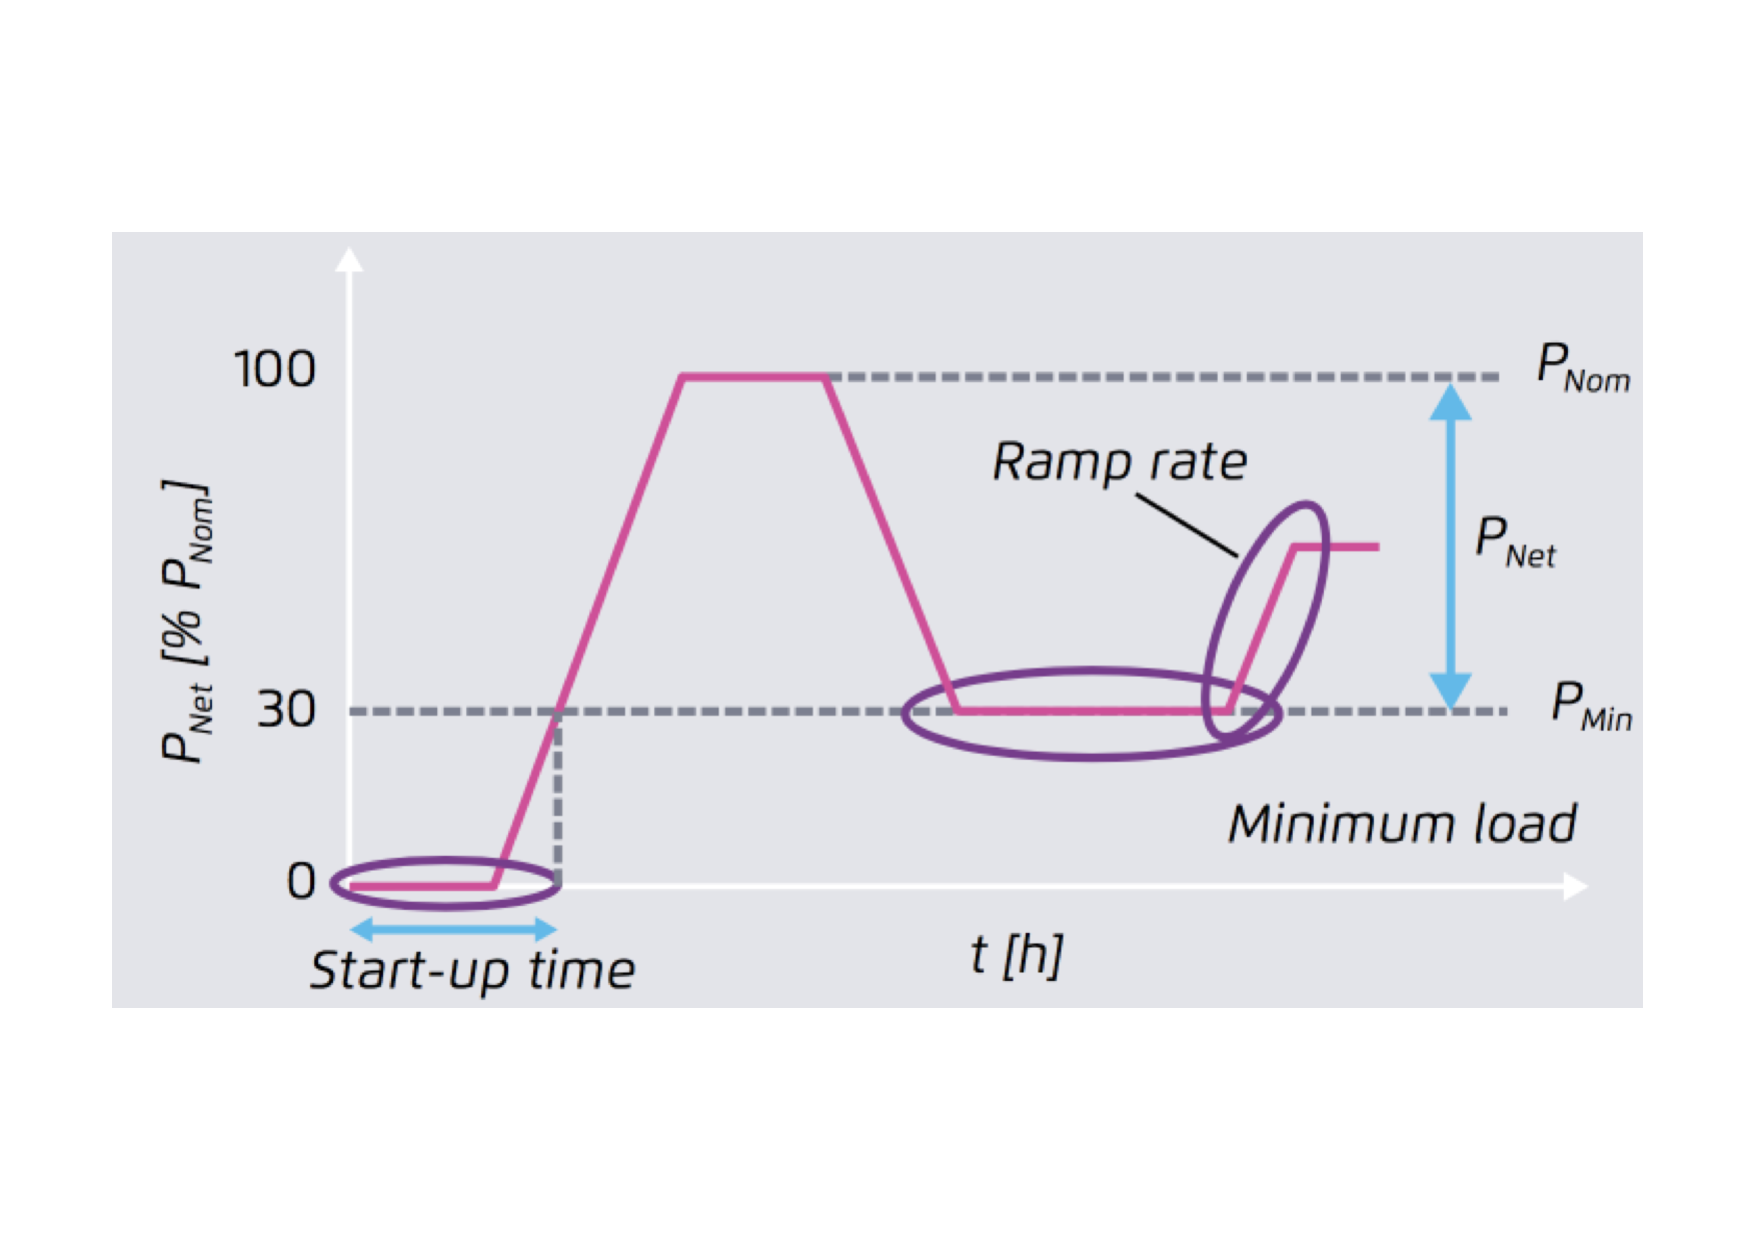
\includegraphics[scale=0.4]{Figures/PowerPlantFlexibility.pdf}
	\caption{Qualitative representation of key flexibility parameters of a power plant\cite{AgoraEnergiewende2017}}\
\end{figure}

The flexibility of a power plant can be characterized by three key features\cite{AgoraEnergiewende2017} (Figure \ref{fig:power-plant-flexibility}): 
\begin{itemize}
	\item Overall bandwidth of operation: the range of output between minimum and maximum load;
	\item Ramp rate: the speed of adjusting output;
	\item Start-up time: the time required to attain stable operation from standstill
\end{itemize}

%https://www.researchgate.net/profile/Alejandro_Hoese
If a power plant can adjust its load from zero to nominate capacity within a time block in the day-ahead market (typically 1 hour), it can be deemed with infinite flexibility in the day-ahead market. This applies to most type generations including solar, wind, hydro and electrochemical systems, etc., except for generations using steam turbines \cite{AgoraEnergiewende2017}, including nuclear, coal-, oil and gas-steam, etc. The gas turbines can be ramped up to full capacity within typically 30 minutes\cite{Siemens}\cite{GE} so can be considered as flexible generation.

For a steam-turbine power plant, the minimum operational load is about 25-60\% of its nominal capacity while the time required to start from standstill is longer than 2 hours \cite{AgoraEnergiewende2017}. Therefore, they are treated as limited flexible sources.

For limited flexible generations, an empirical analysis is performed to determine its bounded flexibility. The procedure for a certain generation source is decribed as following and shown as Figure \ref{fig:bounded-flexibility}:

\begin{figure}[h!]
	\label{fig:bounded-flexibility}
	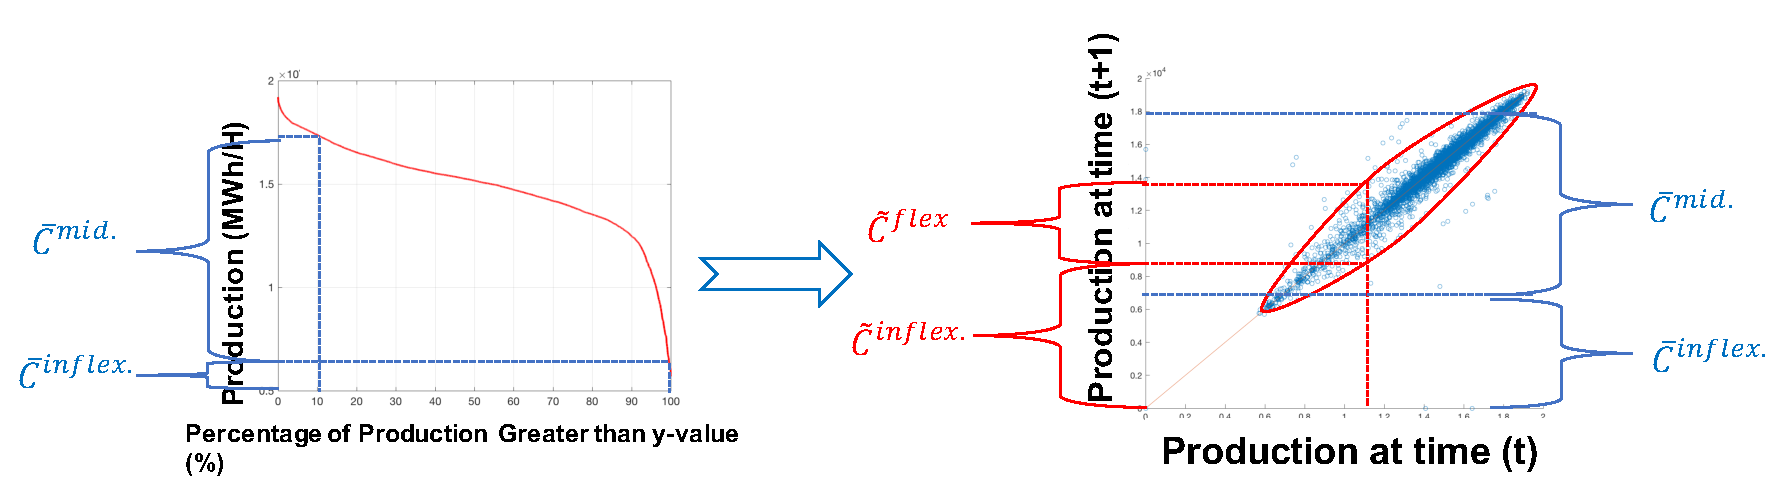
\includegraphics[scale=0.4]{Figures/BoundedFlexibility.pdf}
	\caption{Schematic illustration of determining bounded flexibility for limited flexible generations}\
\end{figure}


\begin{enumerate}
	\item Make the duration curve of the generation data, and obtain $\overline{c}^{mid.}$ which is the range that the generation source is operating for over 10-99\% of the overall period and $\overline{c}^{inflex.}$ which is the range that the generation is operating of more than 99\% of the time.
	\item Determine the envelop lines which limit the production at time $t+1$ based on production at time $t$. With a certain production $p_{t}$, $p_{t+1}$ is bounded within $\tilde{c}^{flex}$, and there is a range of production $\tilde{c}^{inflex}$ that is not economically viable to be curtailed.
	\item Finally, we find the relationship that map the production at time $t$ to flexible capacity at time $t+1$ as: 
	\begin{equation}
	\begin{aligned}
	c^{inflex.}_{t+1} &= \mathcal{C}^{inflex}(p_t)\\ &=max\{\tilde{c}^{inflex.}_t,~\overline{c}^{inflex.}\}
	\end{aligned}
	\end{equation}
	\begin{equation}
	\begin{aligned}
	c^{flex.}_{t+1} &= \mathcal{C}^{flex.}(P_t) \\ & =min\{\tilde{c}^{flex.}_t+\tilde{c}^{inflex.}_t,~\overline{c}^{mid.}+\overline{c}^{flex}_t \} - \tilde{c}^{inflex.}_t
	\end{aligned}
	\end{equation}
	\begin{equation}
	\begin{aligned}
	c^{peak}_{t+1} &= \mathcal{C}^{peak}(P_t) \\ & =max\{\tilde{c}^{flex.}_t+\tilde{c}^{inflex.}_t -(\overline{c}^{mid.}+\overline{c}^{flex}_t),0 \}
	\end{aligned}
	\end{equation}
\end{enumerate}

When the load exceeds the flexible range of these sources, they are no long able to participate in the bidding so these portion of capacity shall be deducted from the overall capacity for the calculation using Equation \eqref{eq:merit-order-model}.

Finally, a regression is performed to determine the parameters in Equation \eqref{eq:merit-order-model} using empirical observations. The errors between a regressed value $\pi_t$ and an actual value $\tilde{\pi}_t$ would be analyzed as the uncertainty of price movement and used for risk controlling as is discussed in risk module. 

With a established merit-order model for day-ahead energy market, we can re-simulate the price with changed market condition, e.g. altered generation capacity mix.

\subsubsection{Real-time energy market and reserve market}

In electricity markets, large portion of energy is usually traded in day-ahead market \cite{Kardakos2013}. There are significate dependences of the real-time (intraday, balancing) energy price on day-ahead price \cite{Woo2016}. Therefore, for real-time energy prices, we adopt a simplex empirical analysis based on comparing the results from day-ahead price simulation and actual market data:

\begin{equation}
\pi^{RT}_t = \kappa (\pi^{DA}_t + \alpha) + \epsilon_t
\end{equation}
where, $\kappa$ and $\alpha$ are terms to adjust the determinate bias between day-ahead and real-time price, while $\epsilon_t$ represents the stochastic movement of real-time price. 

For reserve market, only an empirical model is used as is discussed previously.

\subsection{Market constraints}

The market constraints are a list of limits to make sure that the operation of flexibility resource (determined by $X$ in Equation \eqref{eq:decision-variable-1}) would not violate the actual market rules and market conditions.

Generally, these constraints can be formulated as

\begin{equation}
\begin{bmatrix}
\Gamma^d~~|& \Gamma^c~~|&\Gamma^r
\end{bmatrix}
X \leq \textit{\textbf{b}}
\end{equation}

Most of the market constraints are derived from the market rules so will be introduced in case studies where specific markets are being studies. 

%Capacity constraints:
%\begin{equation}
%r_t^j \leq \hat{r}_t^j ~~~ j \in J
%\end{equation}

%Since in this study high penetration of flexibility resources will be investigated, 

%Day-ahead
%\begin{equation}
%\hat{e}_t^i - \hat{e}_t^{peak} \leq e_t^{d,i} - e_t^{c,i} \leq \hat{e}_t^i - \hat{e}_t^{base} ~~~ i \in \{Day~Ahead\}
%\end{equation}

%Real-time
%PJM revised order +/- 10% of the DA offer
%Germany volume limited





\section{Technology-based modules}

\subsection{Cost module}
\label{sec:cost}
In this thesis, we categorize all costs into two groups: operation-independent and operation-dependent costs.

\subsubsection{Operation-independent costs}
The first group mainly including the initial capital outlay for purchasing the devices and systems, plus the fixed operating and maintenance (O\&M) costs which include miscellaneous items such as the insurance, employee salaries, etc. 

The initial capital cost for a storage system can be divided into two components: an energy-based component, approximately linear to the energy capacity of the system (denoted $\overline{s}$, in MWh), and a power-based component, approximately linear to the power rate of the system (denoted $\overline{r}$, in MW) \cite{Megel2017}. Additionally, we add a component representing the size-invariant costs such as the cost for software. Thereby, the initial capital cost can be computed as:

\begin{equation}
C^{ini} = C^s \overline{s} + C^r \overline{r} + C^0
\end{equation}

where, the coefficients can be obtained empirically either by screening actual market data or from literature. In addition, since the system cost for battery storage is falling rapidly, a learning rate of \textit{ca.} 14\% per annum can be taken to build future scenarios\cite{Nykvist2015}.

The initial capital cost is then annualized by using the concept of equivalent annual cost (EAC):

\begin{equation}
C^{EAC} = \frac{C^{ini}}{\frac{1 - \frac{1}{(1+r)^a}}{r}}
\end{equation}

where $r$ is the discount rate and $a$ is the lifespan of the system in number of years.

The discount rate can be established from the Weighted Average Cost of Capital (WACC) which depends on the financial conditions of different players. A typical WACC in the United States is \textit{ca.} 4-6\% for a municipal utility, 7-8\% for a regulated utility and over 10\% for independent power producer\cite{Rastler2010}. In this study, a discount rate of 10\% is taken unless otherwise stated.

For fixed O\&M costs, $C^{fO\&M}$ which is difficult to calculate precisely, an assumption of 2\% of the initial capital cost is taken, referring to \cite{Rastler2010}. The fixed O\&M costs are added directly to the annualized capital cost to get the total fix costs (in \$/year):

\begin{equation}
C^{fix} = C^{EAC} +  C^{fO\&M}
\end{equation}

The annualized fix cost will finally be compared with the operating revenue calculated from other module to assess the profitability.

\subsubsection{Operation-dependent costs}

Operation-dependent costs primarily refer to the degradation costs, which is specially an issue for battery-based energy storage systems\cite{Barre2013}.

However, as has been reviewed and analyzed in \cite{Megel2017}, there exists no single degradation model that is widely accepted among the literature and applicable for all cases, due to the complexity of this problem. The reasons can be summarized as following:
\begin{itemize}
	\item Modelling battery degradation itself is a complex engineering problem as it is affected by a list of physical parameters, including the degree-of-discharge (DoD), state-of-charge (SoC), charging/discharging rate, temperature, etc.\cite{Barre2013}
	\item The choice of degradation model affects the convex relaxation when degradation effects are included in an optimization problem, the model selection is driven by the requirements of mathematical realization. \cite{Megel2017}
\end{itemize}

Degradation costs can be neglected while operating life time is longer than designed life time, which is generally valid for non-battery energy systems \cite{Bradbury2014}\cite{Zafirakis2016}\cite{Connolly2011}. Some research works studying battery system also made the same assumption  \cite{Byrne2012}\cite{McConnell2015}\cite{Sioshansi2009}. The breakeven point of operational frequency where the degradation of battery storage system can be ignored was concluded to be less than 0.5-1.5 full-cycle equivalent energy throughput per day\cite{Megel2017}. Nonetheless, it was also pointed out by \cite{Megel2017} that while assuming degradation cost being zero, the operational planner would tend to operate the system more frequently, which would possibly in turn to violate the assumption of zero-degradation.

Such a combined investment and operation problem is hard to be incorporated in an optimization, so in our study we first use a simple degradation cost model where the cost is linear to the \textit{energy throughput} $|e^t|$ as a damping term in the optimization and examine it \textit{ex-post}, i.e. if the actual operating life is not reached the degradation cost will be exempted from the final profit calculation. A linear relationship between the degradation and $|e^t|$ is a common technique used in researches for estimating battery degradation\cite{Byrne2012}\cite{Berrada2016}.

Denoting the damping factor for degradation as $\zeta$, we can formulate the degradation damping as:

% THIS IS WRONG
\begin{equation}
\label{eq:degradation-damping}
C^{degradation}_t = \zeta (\sum_{i}^{i \in I}(e_t^{d,i}+e_t^{c,i})+\sum_{j}^{j \in J}(\delta_t^{j,+}+\delta_t^{j,-})r_t^j)
\end{equation}

where, the energy to reserve ratios are separated to positive and negative components:
\begin{equation}
\label{eq:ratio-pos}
\delta_t^{j,+} = \begin{cases}
\delta_t^j & \delta_t^j  \geq 0\\
0 & \delta_t^j  < 0
\end{cases}
\end{equation}
\begin{equation}
\label{eq:ratio-neg}
\delta_t^{j,-} = \begin{cases}
0 & \delta_t^j  \geq 0\\
-\delta_t^j & \delta_t^j  < 0
\end{cases}
\end{equation}

It can be noticed that when a virtual arbitrage is conducted where some $e_t^{d,i}$ and $e_t^{c,i}$ are offset, it will activate the degradation damping with Equation \eqref{eq:degradation-damping} while there are no real physical processes causing degradation. This will be corrected in final profit calculation but in decision making process using optimizations we keep it as it is intended to restrict the virtual arbitrage.

Similar to Equation \eqref{eq:decision-f-revenue-end}, we reconstruct the diagonal matrices with the decomposed ratios from Equation \eqref{eq:ratio-pos} and \eqref{eq:ratio-neg}.
\begin{equation}
\Delta^+ = diag (
\delta_1^{J(1),+}, \dots , \delta_T^{J(1),+}, \dots, \delta_1^{J(|J|),+}, \dots, \delta_T^{J(|J|),+})
\end{equation}
\begin{equation}
\Delta^- = diag (
\delta_1^{J(1),-}, \dots , \delta_T^{J(1),-}, \dots, \delta_1^{J(|J|),-}, \dots, \delta_T^{J(|J|),-})
\end{equation}

The matrix of coefficient for degradation is the derived complying with the form of market modules:

\begin{equation*}
Cost^{degradation} = \begin{bmatrix}
Z^{I}~|~&Z^{I}~|~& \zeta (\Delta^{+} +\Delta^{-})
\end{bmatrix} \begin{bmatrix}
E^d \\ E^c \\ R
\end{bmatrix}
\end{equation*}

where,
\begin{equation*}
Z^I = \begin{bmatrix}
Z^{I(1)}~~|&\dots~~|&Z^i~~|&\dots~~|&Z^{I(|I|)}
\end{bmatrix}~~~
Z^i = \zeta \cdot I_{T\times T} ~~~ \forall i \in I
\end{equation*}

$I_{T \times T}$ is a ($T \times T$) identity matrix. 

\subsection{Technology simulation module}
The technology simulation is applied to determine the state of the system, which would be used primarily for calibration of technology constraints but also for \textit{ex-post} analysis.

\subsubsection{Energy Storage}
Regardless of the type of technology, an energy storage system consists of three functional units, i.e. power input, power output, and storage. Each function unit is associated with an efficiency, i.e. conversion efficiencies of charging, discharging and storage efficiency, denoted as $\eta_c$, $\eta_d$ and $\eta_s$ respectively.

Since the ramp up time for a typical storage system is neglectable comparing to the time resolution in our study, the state of power input and output are deemed as strictly following the operational plan without transient process.

For the state of storage, we define a term, $s$ (in MWh), which is the energy stored in the device, i.e. the State-of-Charge (SoC) multiplied by its maximum energy capacity. The state is determined using Equation \ref{eq:tech-ESS}.

\begin{equation}
\label{eq:tech-ESS}
s_t = \eta_s s_{t-1} + \eta_c (\sum_{i}^{i \in I} e_t^{c,i} + \sum_{j}^{j \in J}\delta_t^{j,-}r_t^j)- \frac{1}{\eta_d} (\sum_{i}^{i \in I} e_t^{d,i} + \sum_{j}^{j \in J}\delta_t^{j,+}r_t^j)
\end{equation} 

In order to formulate Equation \eqref{eq:tech-ESS} in matrix form, we first introduce a matrix denoted $H$:
\[
H
=
\begin{bmatrix}
\eta_s^0 & 0 & 0 &  \dots & 0 \\
\eta_s^1 & \eta_s^0 & 0 &  \dots & 0 \\
\eta_s^2 & \eta_s^1 & \eta_s^0 &  \dots & 0 \\
\vdots & \vdots & \vdots &  \ddots & \vdots \\
\eta_s^{T-1} & \eta_s^{T-2} & \eta_s^{T-3} & \dots & \eta_s^0 \\
\end{bmatrix}
\]
\newline
Then $M$ is used to construct $H^I$ and $H^J$ with a given pair of sets of market segments $I$ and $J$.
\begin{equation*}
H^I = \begin{bmatrix}
H^{I(1)}~~|&\dots~~|&H^i~~|&\dots~~|&H^{I(|I|)}
\end{bmatrix}~~~
H^i = H ~~~ \forall i \in I
\end{equation*}
\begin{equation*}
H^J = \begin{bmatrix}
H^{J(1)}~~|&\dots~~|&H^j~~|&\dots~~|&H^{J(|J|)}
\end{bmatrix}~~~
H^j = H ~~~ \forall j \in J
\end{equation*}
Finally, we can derive the matrix form of Equation \eqref{eq:tech-ESS}.
\begin{equation}
\label{eq:tech-ESS-M}
S = \eta_s H S_0 + \begin{bmatrix}
-\frac{1}{\eta_d} H^I~~|& \eta_c H^I~~|& H^J (-\frac{1}{\eta_d} \Delta^{+} + \eta_c \Delta^{-})
\end{bmatrix} X
\end{equation}
where, $S$ and $S_0$ are vectors for the temporal and initial state, respectively.
\begin{equation*}
S = \begin{bmatrix}
s_1~~s_2~~\dots~~s_T
\end{bmatrix}^T
\end{equation*}
\begin{equation*}
S_0 = \begin{bmatrix}
s_0~~s_0~~\dots~~s_0
\end{bmatrix}^T
\end{equation*}

In order to make it more compact, we reformulate Equation \eqref{eq:tech-ESS-M} as:

\begin{equation}
\label{eq:state-ESS-M-1}
S = \textit{\textbf{h}}_0 + \textit{\textbf{h}}~X
\end{equation}
where
\begin{equation}
\label{eq:state-ESS-M-2}
\textit{\textbf{h}}_0 =  \eta_s H S_0
\end{equation}
\begin{equation}
\label{eq:state-ESS-M-3}
\textit{\textbf{h}} = \begin{bmatrix}
-\frac{1}{\eta_d} H^I~~|& \eta_c H^I~~|& H^J (-\frac{1}{\eta_d} \Delta^{+} + \eta_c \Delta^{-})
\end{bmatrix}
\end{equation}
\subsubsection{Electric Vehicle}

%Charging rate: https://www.tesla.com/support/home-charging-installation
Electric vehicle to grid systems are fundamentally battery energy storage systems in term of their physical dynamics. Therefore, they can be modeled generally using the same approach as in preceding paragraphs. However, there are several attributes that uniquely characterize electric vehicle to grid systems compared to normal battery storages:

\begin{itemize}
	\item The availability of an EV2G system, in terms of delivering both energy (in MWh) and capacity reserve (in MW), is dynamic rather than static, since the number of EVs connected in the power grid is changing all the time with the behaviors of plug-in/ plug-out.
	\item The energy stored in the system will be consumed not only for delivering our targeted services (arbitrage or balancing), but also for driving of EVs themselves. This part of costs will be implicitly captured by the revenue module using Equation \eqref{eq:module-revenue}, which will distort the real value of services provided for the grid. 
\end{itemize}

Therefore, two main modifications are made to adapt the model of ESSs for better representing the EV2G systems: 

\begin{enumerate}
	\item The EV2G system is modeled as a dynamic ESS by taking into consideration the connection/ disconnection of EVs to/ from the grids.
	\item The costs of energy consumed for driving are accounted, following the original plan, i.e. without controlling algorithm for grid services, and added back to the revenue in Equation \eqref{eq:module-revenue}.
\end{enumerate}

In order to implement the first measure, we introduce additional terms to represent the number of EVs entering ($n_t^+$), leaving ($n_t^-$) and remain in ($n_t$) the system at each time step. 
\begin{equation}
\label{eq:EV-number}
n_t = n_{t-1} + n_t^+ - n_t^-
\end{equation}

Thereby the state equation for an EV2G system is written as:
\begin{equation}
\label{eq:tech-EV}
\begin{aligned}
s_t = & \eta_s s_{t-1} + \eta_c (\sum_{i}^{i \in I} e_t^{c,i} + \sum_{j}^{j \in J}\delta_t^{j,-}r_t^j)- \frac{1}{\eta_d} (\sum_{i}^{i \in I} e_t^{d,i} + \sum_{j}^{j \in J}\delta_t^{j,+}r_t^j) \\
&+ s_t^+ n_t^+ - s_t^- n_t^-
\end{aligned}
\end{equation} 
\newline
The matrix form of Equation \eqref{eq:EV-number} is as following:
\begin{equation}
\label{eq:EV-number-M}
N = I_{T \times T} N_0 + L_{T \times T} N^+ -L_{T \times T} N^- 
\end{equation}
where, $L_{T \times T}$ is a ($T \times T$) identity lower triangular matrix. The rest matrices are defined as following
\begin{equation*}
N = \begin{bmatrix}
n_1~~n_2~~\dots~~n_T
\end{bmatrix}^T
\end{equation*}
\begin{equation*}
N_0 = \begin{bmatrix}
n_0~~n_0~~\dots~~n_0
\end{bmatrix}^T
\end{equation*}
\begin{equation*}
N^+ = \begin{bmatrix}
n_1^+~~n_2^+~~\dots~~n_T^+
\end{bmatrix}^T
\end{equation*}
\begin{equation*}
N^- = \begin{bmatrix}
n_1^-~~n_2^-~~\dots~~n_T^-
\end{bmatrix}^T
\end{equation*}
\begin{equation*}
S^+ = diag(s_1^+, s_2^+, \dots, s_T^+
)
\end{equation*}
\begin{equation*}
S^- = diag(s_1^-, s_2^-, \dots, s_T^-)
\end{equation*}
\newline
Analogously, translating Equation \eqref{eq:tech-EV} to matrix form leads to:

\begin{equation}
\begin{aligned}
S = &~ \eta_s H S_0 + H S^+ N^+ - H S^- N^- \\
&~+ \begin{bmatrix}
-\frac{1}{\eta_d} H^I~~|& \eta_c H^I~~|& H^J (-\frac{1}{\eta_d} \Delta^{+} + \eta_c \Delta^{-})
\end{bmatrix} X
\end{aligned}
\end{equation}
which can be reformulated as:
\begin{equation}
\label{eq:state-EV-M-1}
S = \textit{\textbf{h}}_0 + \textit{\textbf{h}}~X
\end{equation}
where
\begin{equation}
\label{eq:state-EV-M-2}
\textit{\textbf{h}}_0 =  \eta_s H S_0 + s^+ H N^+ - s^- H N^-
\end{equation}
\begin{equation}
\label{eq:state-EV-M-3}
\textit{\textbf{h}} = \begin{bmatrix}
-\frac{1}{\eta_d} H^I~~|& \eta_c H^I~~|& H^J (-\frac{1}{\eta_d} \Delta^{+} + \eta_c \Delta^{-})
\end{bmatrix}
\end{equation}

\subsection{Technology constraints}
\label{sec:tech-constraints}
The technology constraints are set to ensure the operation plan is fulfilled physically by the system.

\subsubsection{Energy storage}
Firstly, the charging/ discharging rate shall be bounded at its maximum rate ($\overline{r}$, assuming symmetric for charge and discharging).

\begin{equation}
0 \leq \frac{1}{\Delta t}\sum_{i}^{i \in I} e^{d,i}_t + \sum_{j}^{j \in J} r_t^j \leq \overline{r}~~~ \forall t \in T
\end{equation}

\begin{equation}
0 \leq \frac{1}{\Delta t}\sum_{i}^{i \in I} e^{c,i}_t + \sum_{j}^{j \in J} r_t^j \leq \overline{r}~~~ \forall t \in T
\end{equation}

It can be noticed that opposite movement of charging/ discharging in different markets are not offset in the constraints. This implies virtual arbitrageurs are not allowed to make deals that cannot be afforded physically although the physical systems are not actually activated.

Meanwhile, the energy stored is restricted as well.

\begin{equation}
0 \leq s_t \leq \overline{s}~~~ \forall t \in T
\end{equation}

Replacing $s_t$ using Equation \eqref{eq:tech-ESS}, the contraint is formulated as:
\begin{equation}
0 \leq \eta_s s_{t-1} + \eta_c (\sum_{i}^{i \in I} e_t^{c,i} + \sum_{j}^{j \in J}\delta_t^{j,-}r_t^j)- \frac{1}{\eta_d} (\sum_{i}^{i \in I} e_t^{d,i} + \sum_{j}^{j \in J}\delta_t^{j,+}r_t^j) \leq \overline{s}
\end{equation}

Applying the matrix format of the equations, we can get the constraints re-formulated the constraints of rates as:

\begin{equation}
- \frac{1}{\Delta t} \begin{bmatrix}
\overbrace{ I_{T\times T}|\dots|I_{T\times T}}^\text{|I|}|\overbrace{O_{T\times T}|\dots|O_{T\times T}}^\text{|I|}|\overbrace{ I_{T\times T}|\dots|I_{T\times T}}^\text{|J|}| 
\end{bmatrix} X \leq 0
\end{equation}

\begin{equation}
- \frac{1}{\Delta t} \begin{bmatrix}
\overbrace{ O_{T\times T}|\dots|O_{T\times T}}^\text{|I|}|\overbrace{I_{T\times T}|\dots|I_{T\times T}}^\text{|I|}|\overbrace{ I_{T\times T}|\dots|I_{T\times T}}^\text{|J|}| 
\end{bmatrix} X \leq 0
\end{equation}

\begin{equation}
\label{constraint:ESS-capacity}
\frac{1}{\Delta t} \begin{bmatrix}
\overbrace{ I_{T\times T}|\dots|I_{T\times T}}^\text{|I|}|\overbrace{O_{T\times T}|\dots|O_{T\times T}}^\text{|I|}|\overbrace{ I_{T\times T}|\dots|I_{T\times T}}^\text{|J|}| 
\end{bmatrix}X \leq \overline{R}
\end{equation}
\begin{equation}
\label{constraint:ESS-capacity-2}
\frac{1}{\Delta t} \begin{bmatrix}
\overbrace{ O_{T\times T}|\dots|O_{T\times T}}^\text{|I|}|\overbrace{I_{T\times T}|\dots|I_{T\times T}}^\text{|I|}|\overbrace{ I_{T\times T}|\dots|I_{T\times T}}^\text{|J|}| 
\end{bmatrix}X \leq \overline{R}
\end{equation}

where $O_{T \times T}$ is a $T \times T$ zero matrix and
\begin{equation*}
\overline{R} = \begin{bmatrix}
\overbrace{\overline{r}, \dots, \overline{r}}^\text{T}
\end{bmatrix}^T
\end{equation*}


The constraints of storage are formulated as:
\begin{equation}
\label{constraint:ESS-energy-1}
-\textit{\textbf{h}}~X \leq \textit{\textbf{h}}_0
\end{equation}
\begin{equation}
\label{constraint:ESS-energy-2}
\textit{\textbf{h}}~X \leq \overline{S} -  \textit{\textbf{h}}_0
\end{equation}
where, $\textit{\textbf{h}}$ and $\textit{\textbf{h}}_0$ are determined by Equation \eqref{eq:state-ESS-M-1} to \eqref{eq:state-ESS-M-3}, and
\begin{equation*}
\overline{S} = \begin{bmatrix}
\overbrace{\overline{s}, \dots, \overline{s}}^\text{T}
\end{bmatrix}^T
\end{equation*}

\subsubsection{Electric vehicle to grid}

The constraints for ESS are generally portable for the EV2G systems, by simplying re-using Equation \eqref{eq:state-EV-M-1} to \eqref{eq:state-EV-M-3} to derive $\textit{\textbf{h}}$ and $\textit{\textbf{h}}_0$, and replacing the upper bound limit in Equation \ref{constraint:ESS-capacity} with

\begin{equation}
\overline{R} = \overline{r}N
\end{equation}
where, $N$ is determined by Equation \eqref{eq:EV-number-M}. 




\section{Optimization Engine}
The performance of a flexibility resource depends primarily on the operation plan, which is represented as $X$ (Equation \ref{eq:decision-variable-1}). In order to value the market of technology vendors supplying flexibility to actors in power markets, we need to find reasonable operation patterns that simulate the behaviors of those players. For this sake, we employ an optimization engine. The value of market calculated with the results from optimization stands for the upper bound of market value.

The objective function of the optimization problem is formulated as:
\begin{equation}
\underset{X}{max} \left[ (1-\beta)\left(Revenue (X) - C^{degradation}(X)\right) - \beta CVaR(X) \right]
\end{equation}
where, X is the vector of decision variables (Equation \eqref{eq:decision-variable-1}), and $Revenue$, $C^{degradation}$ and $CVaR(X)$ are calculated using the equations in corresponding modules. $\beta$ is a weighting parameter with $\beta \in [0,1]$, which is used to study the trade-off between profit and risk.

The constraints have been introduced in the modules of market and technology constraints.

The optimization is implemented in MATLAB\textcopyright~and solved using Guobi optimizer. 

\section{Addtional measures for special cases}
\label{sec:special}

\subsection{Backcast technique to reduce the predictability of price}
As has been discussed in the literature review, many of the researches on arbitrage of flexibility in power markets assume the players have perfect foresights of future price movement, which would lead to an over-estimate of the real market value. Reducing the length of predictable window, using 'backcast' technique, and introducing stochastic programming are the usual choices to deal with this issue.

In this thesis, although the players would suffer risks of uncertain price movement with the introduction of stochastic part of price, they were still assigned with full foresight of the probability distribution. One may argue this is also unrealistic and could probably over-estimate the market potential. Therefore, by extending the work \cite{Drury2011} and \cite{Sioshansi2009}, we preformed a sensitivity analysis with reduced predictability using backcast.

We assume the way players predict the short-term forecast of future price is using the following equation:

\begin{equation}
\hat{\pi}_t = \hat{\pi}_{t-t_w} \cdot \frac{\sum_{t-t_w+1}^{t-t_d}\pi_{\tau}}{\sum_{t-t_w-t_w+1}^{t-t_w - t_d}\pi_{\tau}}
\end{equation}
where, $t_w$ is the time period of one week and $t_d$ is the time of one day. The future price is determined by taking the price curve shape of the day of last week and is adjusted by the 7-days average price level.

\subsection{Coupling day-ahead and real-time energy market}

When we value a case where player can participate in day-ahead and real-time (intraday, balancing) energy markets at the same time, an issue rises as they were assigned with full foresight and could easily leverage this advantage to make virtual arbitrage between day-ahead and real-time markets. Since the virtual arbitrage does not activate any physical process and purely benefited from the unrealistic foresight, it has to be constrained. Some researchers have also noticed this issue and used techniques such as put a proportional constraint of real-time volume to day-ahead volume \cite{Han2017} or deny reserved biddings between day-ahead and real-time market \cite{Berrada2016}.

In this thesis, the virtual arbitrage has already been damped by the degradation model as has been discussed in Section \ref{sec:cost} and restricted by the rate constraints in Section \ref{sec:tech-constraints}. Furthermore, we would perform a two-stage optimization where the day-ahead decisions will be made without knowing the real-time prices and the decisions for real-time market biddings will be determined afterwards to reflect the real market condition. We will compare the impact of virtual arbitrage in sensitivity analysis. 

\subsection{Dealing with non-energy-neutral signal for frequency control}
Providing frequency control is an attractive option for flexibility management as it is more profitable than energy arbitrage in current market context. However, a challenge of performing frequency control with non-generating flexibility sources is the non-energy-neutral signals of frequency regulation. If the control signal is not energy-neutral or not auto-corrected, it is not possible for a non-generating resource to provide service for an extended period due to the limited energy capacity. For example, a battery cannot absorb any more energy while it is fully charged and fail to continue delivering frequency control services.

Although some system operators have already implemented special energy neutral signals for the emerging flexibility resources, it is not a universal practice among the markets. 

In this study, we referred to the similar works \cite{Megel2017}\cite{Oudalov2007}\cite{Borsche2013}\cite{Jin2014} where the biased regulation signals are offset using external measure, e.g. via bilateral transactions or purchasing from the power markets. We assume that actors will purchase energy from the power market with real-time price to neutralize the regulation signal . 

\subsection{Final adjusted profit calculation}
As has been discussed above, we have introduced a list of treatments to better model the problem. However, some of the treatments would distort the perceived profits deviating from actual profits received by the actors, i.e. the differences exist between the value for decision making and for final accounting. Therefore, after performing the optimization, we would use the determined operation plan to re-calculate the profits to get the real values. 

~\newline

\textit{(Descriptions about Data has been moved to the chapter of case study as they are market-specific rather than generic.)}


\chapter{Case Studies}
\section{Analyzing the power market structures and business opportunities in select cases}

PJM: symmetric (self-schedule, pool-auction), obligation (load contributing factor), market-based, imbalance(enforcement, 10\% waved for VRE),

Germany: asymmetric (balancing energy market vs frequency control market), 

AEMO: asymmetric (AEMO pays for provider, charge regulation from either all generators or all consumers, and charge contingency from causer)

\label{sec:qualitative-analysis}
The super-set of I is the set of selected energy market segments in different geographies:

\begin{equation*}
I \subseteq  \begin{cases}
\{Day~Ahead, Real~Time\} & PJM \\
\{Day~Ahead, Intraday, Balancing\} & Germany \\
\{Real~Time\} & NSW
\end{cases}
\end{equation*}

The superset of I is the set of selected reserve market segments in different geographies:

\begin{equation*}
J \subseteq  \begin{cases}
\{RegA, RegD, SR, NSR, DASR\} & PJM \\
\{PCR, SCR+, SCR-, TCR+, TCR-\} & Germany \\
\{Lower, Raise\} \times \{REG, 6SEC, 60SEC, 5MIN\} & NSW
\end{cases}
\end{equation*}

\subsection{PJM}
\subsubsection{Organization of PJM power markets}
Marketplaces
Timeline

\subsubsection{Players}
A Load Serving Entity (LSE), as is defined officially by PJM, is "any entity that has been granted authority or has an obligation pursuant to state or local law, regulation, or franchise to sell electric energy to end-users that are located within the PJM RTO. An LSE may be a Market Buyer or a Market Seller"\cite{PJM2017b}. Therefore, LSEs refer to all market participates in PJM who have rights and obiligation to act in all the power marketplaces of PJM, including the energy, capacity and ancillary services markets. 

Curtailment Service Providers (CSPs) are members in PJM markets specializing in demand response. A CSP is an intermitted agency that provides the end-user DR to the wholesale market. \cite{PJM2017b} \cite{Wang2015} The role of the CSP is actually a legacy product from the liberalization of retail markets in PJM. Once the retail competition began, PJM allowed LSEs to provide DR not only for their own customer but also for customers of other LSEs. The role of the CSP was created to facilitate the liberalization and competition. \cite{PJMInterconnection2017}

\subsubsection{Balancing mechanism}
submit offer - rebid - update information up to 65 mins - deviation charged with real-time

reviewed the participation, violating -> suspend activity, enter enforcement

LSE obiligate to purchase (or self-schedule) reserve, obiligation as a proportion to its contributing flow to the grid. \cite{PJM2017c} This incents liquidity in the market with competitions on both buyer's and seller's side. However, the obiligation does not reflect their actual needs.\cite{Wartsila2014}

CSP
intermitted agency
allowed to voluntarily respond to the LMP

\subsubsection{PJM DR}

PJM DR is the umbrella for all distributed energy resources, including DR, behind-the-meter generations, storage, etc. since PJM does not specify how the load is reduced. However, PJM DR program does not allow energy injection beyond the meter and receive wholesale compensation.\cite{PJMInterconnection2017}. This issue is currently under discussion in Special Market Implementation Committee meetings.

DR emergency fast changing over years \cite{Brown2015}
Since the DR in the wholesale market as a supply recouse will cause double payment issue where a customer may receive wholesale energy revenue and retail cost savings for the same MW of load reduction, PJM states that DR participation in the retail market on the demand side would be more ideal. And they are discussing to revisit the mechanism. Therefore, this value is not fully modeled in our study.

LSE
buyer or seller in Energy, and reserve market

\subsubsection{Identify business model}

\subsubsection{Accounting}





The real-time market price is applied for all deviations from day-ahead planned schedule, including Regulation, Primary and Supplementary Reserves.

\begin{equation*}
\pi_t^{e,j} = \pi_t^{e,i} ~~~~ i \in \{Real~Time\}, j \in \{RegD, RegA, SR, NSR, DASR\}
\end{equation*}

The capacity prices of reserves are computed using a complex algorithm, taking into account a list of specifications of the resource, e.g. the performance \& historical performance, benefits factor, mileage, etc. The detailed calculations can be found in appendix. As outputs, we will get deterministic values for $j \in \{RegA, SR, NSR, DASR\}$, and the upper and lower bounds, $\overline{\pi}_t^{r,j}$ and $\underline{\pi}_t^{r,j}$, for $i \in \{RegD\}$.

%Reg = RMCCP + RMPCP + LOC
%LOC = 0
%RMCCP = 
%RMPCP = Milleage
%Effective MW = BF * MW
%BF is determined with the average and upper, lower bounds

\subsection{Germany}
$\pi_t^{e,i}, i \in \{Balancing\}$, is the the price for balancing energy (reBAP), which exist only in Germany

$\pi_t^{r,j}$ and $\pi_t^{e,j}$ are based on principle of pay-as-bid. The weighted-average values are available in the datasets.

%Market participants in Germany are organised into balancing groups, known as Bilanzkreise (BK). BK can range from individual large generators to aggregations of smaller renewable generations, to a Stadwerke representing large portions of aggregated demand.

%Every balancing group operator is responsible for following a planned schedule with a 15-minute resolution. Deviations from the planned schedule are balanced physically by the TSOs and settled financially with the BK. There is a legal obligation on Bilanzkreise to balance their positions to the best of their ability.

Prices for balacning energy are unified across TSOs and determined according to the  balancing energy price settlement system (BK6-12-024) developed by Federal Network Agency (FNA) as of 01/12/2012.

\begin{equation}
\label{eq:reBAP}
reBAP = \frac{\sum net imbalance energy cost}{\sum net imbalance energy volume}
\end{equation}

\subsection{Australia-New South Walse}
The unit prices of reserve products, $\pi_t^{r,j}$ and $\pi_t^{e,j}$, are not available in datasets published by AEMO. Only weekly summary for total payment and recovery are provided. Due to the limits of available data, we are only able to perform calculations of total potential revenues, rather than thorough studies as in the other two geographies.

\newpage

\section{Quantitative studies and results}
So far we have elaborated qualitatively the existing and potential opportunities for flexibility management in the three geographies, and screened the possible business cases. Further to that, it is necessary to perform quantitative analysis in order to understand:

\begin{itemize}
	\item \textbf{Market Size:} the potential value creation in the market for flexibility management solutions, subject to certain generic system dynamics but without respect to cost dynamics of specific technologies
	\item \textbf{Profitability:} the metric to judge whether a specific technology is profitable or not to extract certain amount of value from current or future markets taking into account cost elements
\end{itemize}

Based on the methodology introduced in Chapter \ref{ch:methodology}, we performed experiments with consideration of constraints from both markets and technologies. All three markets discussed previously and two technologies, i.e. energy storage system (ESS) and Electric vehicle to grid (EV2G), were studied. 

Specifically, the ESS with a system dynamic that is able to release and absorb energy can be deemed as a generic flexibility source. The revenue derived using ESSs can be viewed as a reference of the maximum market potential from flexibility management. Meanwhile, with cost parameters of a typical battery energy storage system (BESS), we can analyze the profitability of BESSs with results involving elements of costs. 

On the other hand, EV2G is served as a more peculiar example of technology, with additional case-specific constraints like the EV driving behaviors compared to a generic ESS. Maximum revenue from this technology shall be bounded by values derived from the generic ESS, but the profits may deviate significantly from values of BESSs, as their cost dynamics and business models could be distinct with other. Details are to be introduced later in this section.

Two types of works were carried out. We first examined the value of markets for flexibility management under current market conditions, i.e. based on historical observations without involving the market simulation module (Section \ref{sec:market-simulation}). This allows us to obtain some concrete numbers to establish a comprehensive understanding toward the value of flexibility management in nowadays' power markets. 

Thereafter, as markets evolve rapidly especially with the disruption of fast-growing renewable generations, a view toward market development is also necessary. As a immature business, valuation of markets for flexibility management would be sensitively affected by various factors. The multi-dimensional variances and unpredictable changes on non-technical issues like market design and regulatory adjustments make it almost impossible to accurately forecast the market size and profits in the future. Nonetheless, understanding the impacts of some key factors would provide us valuable guidance on the directional movement of the market and thus offer viable references for technology vendors' decision makers.

\subsection{Data, parameters and valuation metrics}
The electricity market data including price and volume in each marketplaces correspond to the actual market data from January 1st 2016 to December 31st 2016. While general rules for accounting and data availability have been discussed in Section \ref{sec:qualitative-analysis}, detailed pre-processes and how they were fitted in as inputs of our valuation model can be found in Appendix \ref{sec:accounting-data-prepare}.

For cost determinations, we would first use figures based on the present market pricing level, and then make scenarios with reduced costs to find the break-even point if it is not yet profitable. According to the International Renewable Energy Agency (IRENA)\cite{IRENA2017}, the cost for battery energy storage systems was analyzed as proportional to their energy capacity, $\overline{s}$, and the energy cost coefficient, $C^s$, for state-of-the-art lithium-ion batteries were reported to be ca. $\$350/kWh$ in 2016. The replacement cost were based on actual price from Tesla\cite{Tesla1}, one of the leaders in battery and electric vehicle markets. The operating life is set to be 6000 FCEs, which corresponds to an optimistic estimation by Sandia National Laboratories\cite{Akhil2015}. Designed life time is assumed to be 10 years. Discount rate is made as 10\% as is discussed in Section \ref{sec:cost}. The technology costs were made to be zero so that the derived profits will be the margins that can be possibly realized by technology vendors. All the parameters for cost calculation are summarized in Table \ref{table:cost-parameters}. 

\begin{table}[h!]
	\begin{center}
		\begin{tabular}{ l  l  R{2.7cm} } %R{2.7cm} |}
			\hline
			\textbf{Items} & \textbf{Unit} & \textbf{Value} \\% & \textbf{Reduced Cost} \\
			%\hline
			\hline
			Energy cost coefficient, $C^s$ & $\$/kWh$ & 350 \\%& 140 \\
			%\hline
			Power cost coefficient, $C^r$ & $\$/kW$ & 0\\% & 0 \\
			%\hline
			Technology cos,t $C^0$ &$\$$ & 0\\% &0\\
			%\hline
			Replacement cost coefficient, $C^s$ &$ \$/kWh$ & 150\\% & 60 \\
			%\hline
			Designed life time & \textit{year} & 10\\% \multicolumn{2}{c|}{10}\\
			%\hline
			Operating life time & \textit{FCE} & 6000\\% \multicolumn{2}{c|}{6000}\\
			%\hline
			Discount rate &$\%$ & 10\\% \multicolumn{2}{c|}{10}\\
			\hline
		\end{tabular}
	\end{center}
	\caption{Parameters for cost calculation}\label{table:cost-parameters}
\end{table}

It is worthwhile to point out again that by using the parameters described above, the ESSs are virtually battery energy storage systems (BESSs). This fits the purpose of case studies. However, the conclusions on profitability are not portal for other types of ESS, but it does not mean the methodology loses its generality. The value of revenue would still be valid for other types of technology as long as they can have the same function of shuffling energy between time slots. Furthermore, by using different data as inputs, our model can be utilized for analysis of profitability of other energy storage systems with different cost dynamics. 

\begin{figure}[h!]
	\centering
	\centering
	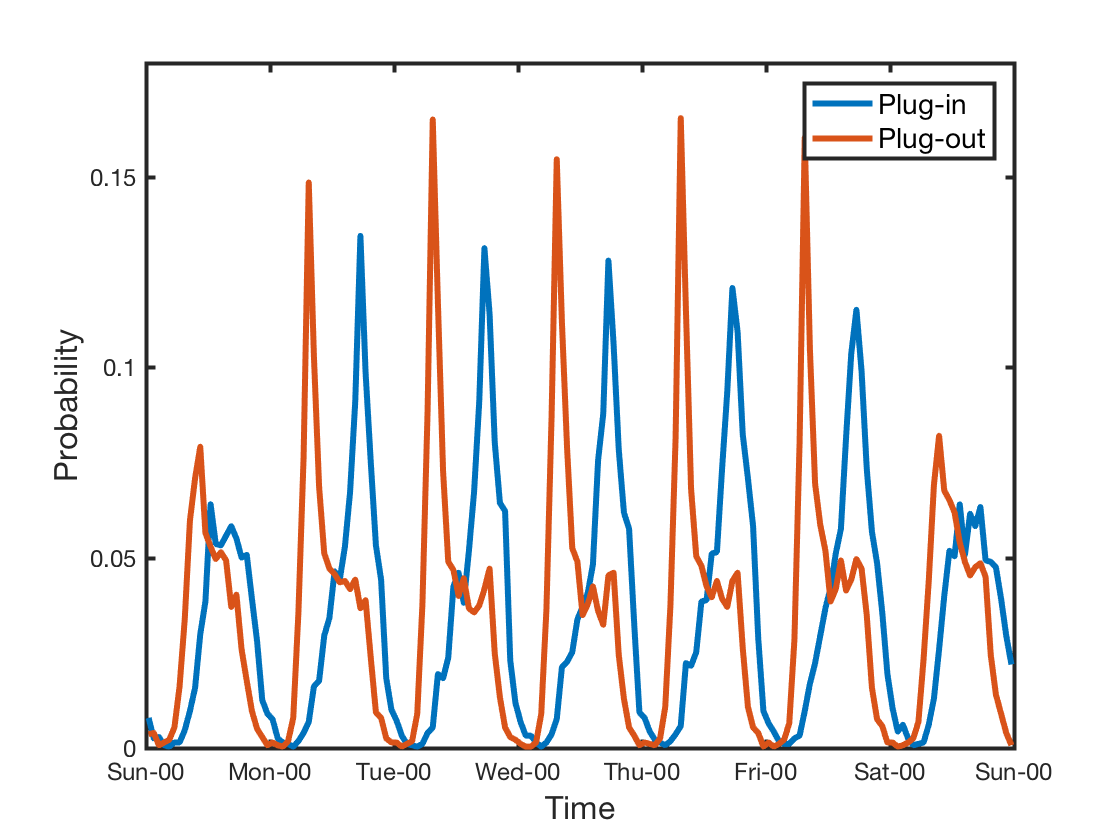
\includegraphics[width=0.8\linewidth]{Figures/Data_EV_number}
	\caption{Probability of EV plug-in/ plug-out}
	\label{fig:data-ev-number}
\end{figure}

\begin{figure}[h!]
	\centering
	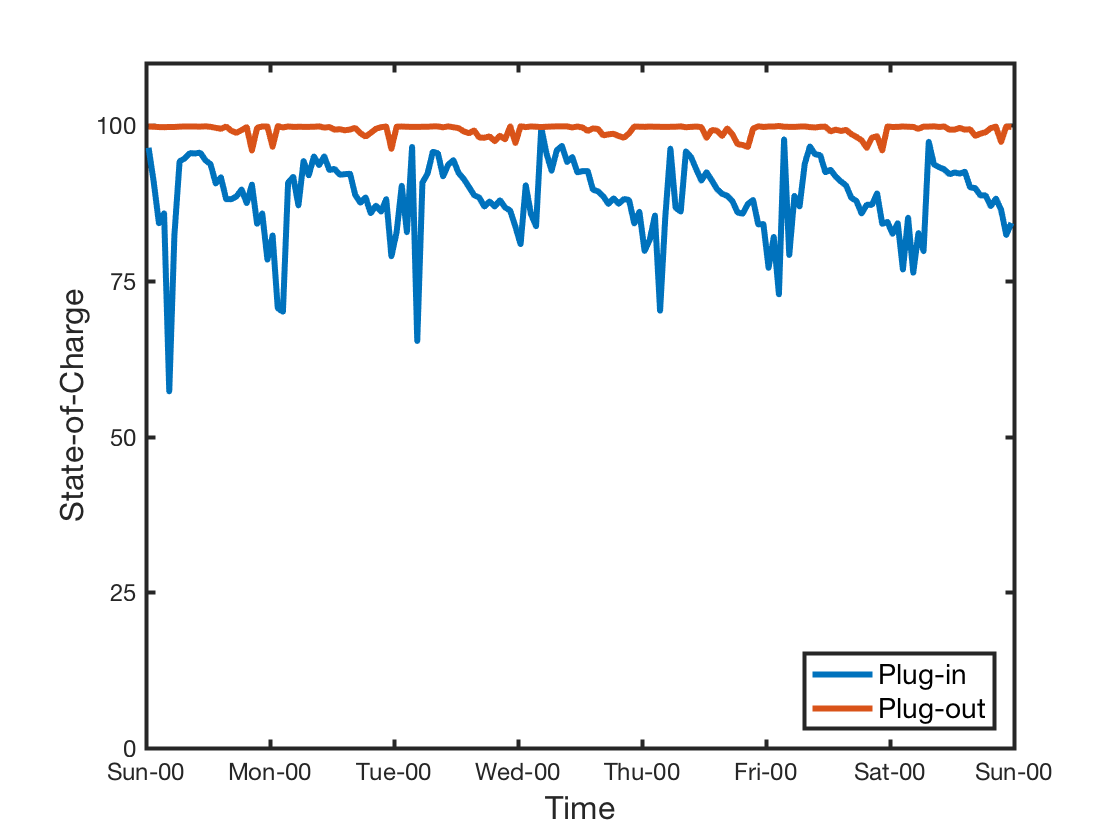
\includegraphics[width=0.8\linewidth]{Figures/Data_SoC}
	\caption{Average SoC of EV when plug-in/ plug-out}
	\label{fig:data-soc}
\end{figure}

In terms of EV2G studies, we first determined the battery parameters of EVs.

\begin{itemize}
	\item EV charging rate is 10kW, corresponding to the guidance provided by Tesla\cite{Tesla2} and a typical home charging infrastructure with 50A current limit. 
	\item The battery energy capacity per EV of 75kWh is taken from one of the most popular EV models\cite{Tesla3}.
\end{itemize}

Simulations are then performed to get EV driving profiles, which are based upon data from the California Department of Transportation's California Household Travel Survey for 2010-2012\cite{NREL_TSDC}. This survey carried out multiple objectives and included 79011 vehicles. For our work we focus on a proportion of the vehicles, 2910, which were fitted with GPS. These vehicles were monitored continuously for a 7-day window with the 1-second resolution. The GPS data is then processed into trip profiles, while include information of the location of each EV at each time step as well as the trips made by each EV. Furthermore, together with the parameters of the EV model we have selected above we simulated the SoC time series of the EV batteries. Finally, from the simulated results, we can statistically derive the value of probability distribution of EV plug-in $n^+$, plug-out $n^-$, and average state-of-charge (SoC) of batteries plug-in $s^+$, plug-out $s^-$, as introduced in Section \ref{sec:tech-simulation-module}. The results are shown as Figure \ref{fig:data-ev-number}-\ref{fig:data-soc} where we can see clear periodic patterns that are different between weekdays and weekends.

The metrics to evaluate the system performance are slightly different between ESS and EV2G. For ESS, the criteria in the evaluation metrics include
\begin{itemize}
	\item \textbf{Revenue:} the total explicit revenue from electricity markets calculated as Equation \eqref{eq:module-revenue} in Section \ref{sec:revenue}, per annum
	\item \textbf{Operating cost:} the operation-dependent costs (essentially degradation cost); refer to Section \ref{sec:cost} and Equation \eqref{eq:degradation-damping}, per annum
	\item \textbf{Operating Profit}: the total revenue net of the operating cost, per annum
	\item \textbf{Fixed cost:} the equivalent annual cost (EAC) of operation-independent costs (essentially expenses on ESS infrastructure); refer to Section \ref{sec:cost}
	\item \textbf{Profit:} the total revenue net of both operation-dependent and fixed costs, per annum
	\item  \textbf{Profitability ratio}: the ratio between the profit and overall costs including both operating and fix costs
\end{itemize}

For EV2G, the fixed cost that is mainly related to procuring the battery stocks shall not be considered for a technology vendor. Furthermore, the implicit charging cost to compensate the energy consumed by EV driving are listed separately. Depending on the specific business model in practice, a portion of the implicit charging cost may be recovered by the technology vendors from the end-users, although in this thesis we did not exclude it from calculating the profit. As a result, the criteria are altered as:
\begin{itemize}
	\item \textbf{Revenue:} the total explicit revenue from electricity markets calculated as Equation \eqref{eq:module-revenue}, per annum
	\item \textbf{Operating cost:} the operation-dependent costs (essentially degradation cost), per annum
	\item \textbf{Implicit Charging Cost}: the cost of energy compensation for EV driving demands, calculated as the total energy consumption multiplied by average price over the span of one operational cycle, per annum
	\item \textbf{Profit:}: revenue net of costs including the implicit charging cost and battery degradation. The investments on technology are made to be zero as is discussed at the beginning of this section, per annum
	\item  \textbf{Profitability ratio}: the ratio between the profit and overall costs including both operating and implicit charging costs
\end{itemize}

As a result, the profit of a EV2G system is closed to the concept of operating profits for a ESS, which excludes the investment of procuring batteries. This implies two disparate business models. Cautions shall be raised while comparisons between these two technologies are made.

In order to determine the profitability and market size of ESS, we evaluated the system performance with different total sizes. Thereafter, we would select some key states in order to extract the most informative indicators to technology vendors. Overall, 4 scenarios would be analyzed and are illustrated by Figure \ref{fig:scenario-illustration} using an example with typical curve shapes. This example shows the results for a case of making arbitrage in day-ahead, real time energy markets and simultaneous delivering regulation services in PJM electricity markets. 
\begin{figure}[h!]
	\centering
	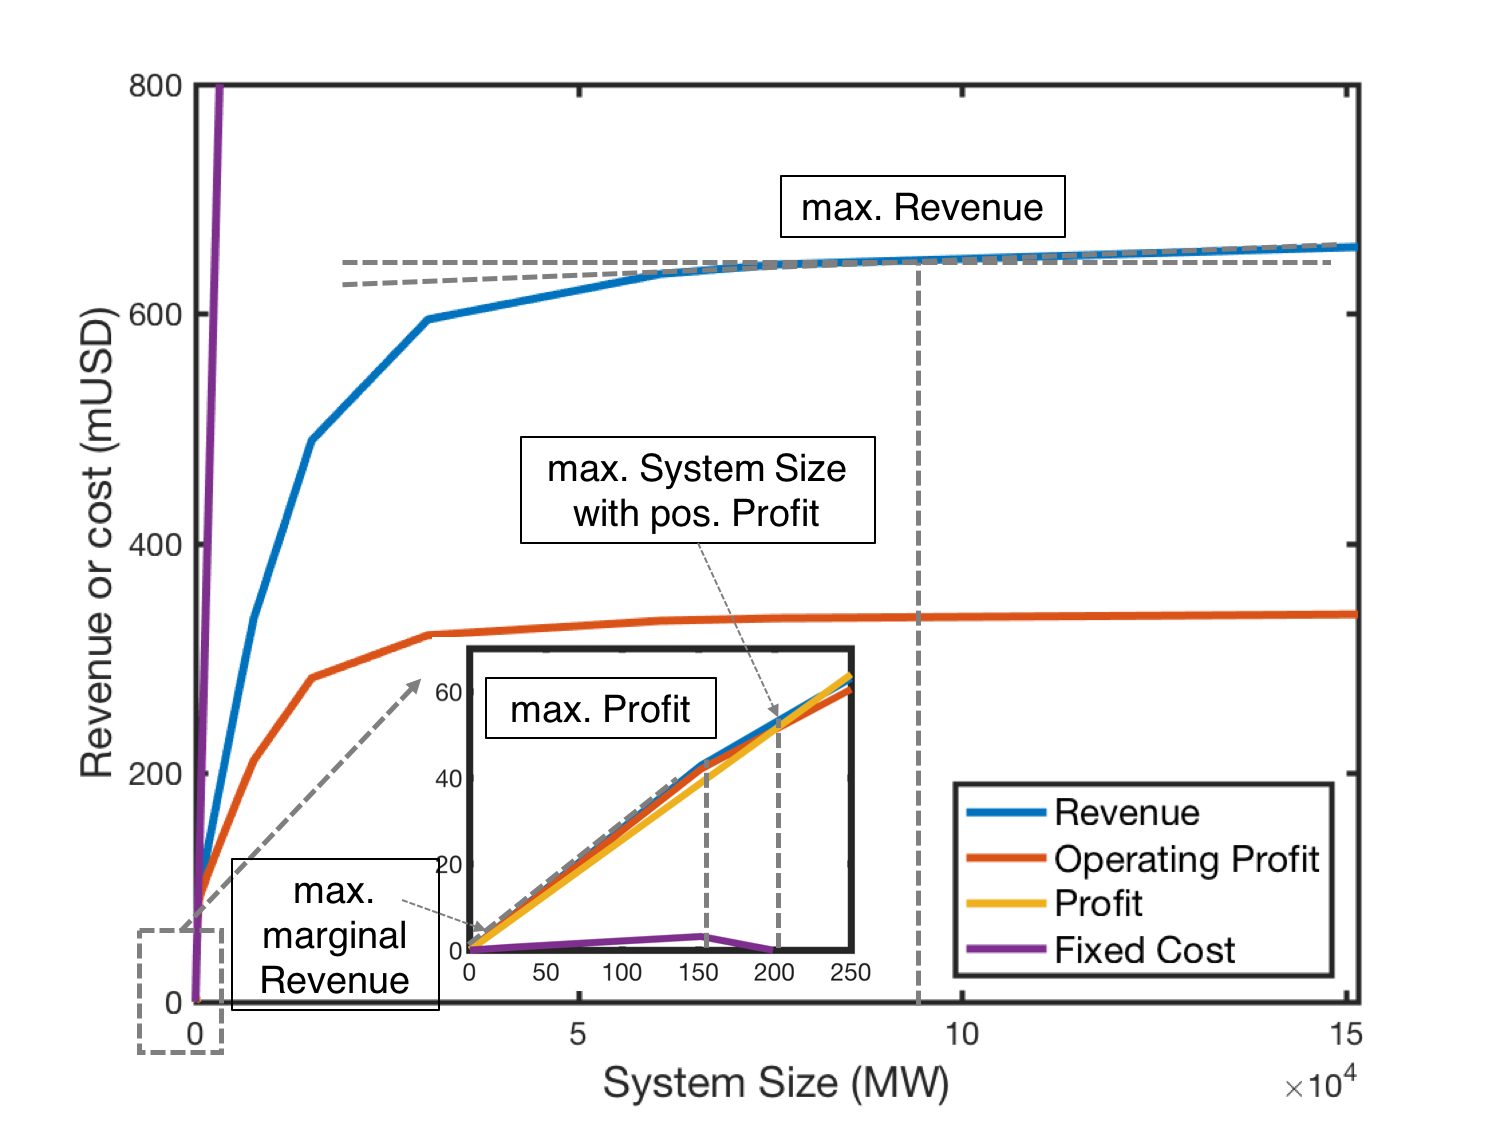
\includegraphics[width=0.95\linewidth]{Figures/Scenario_illustration}
	\caption{Graphic illustration of 4 scenarios}
	\label{fig:scenario-illustration}
\end{figure}

Two the most crucial states are:

\begin{itemize}
	\item ``\textbf{max. Revenue}": the state where the maximum potential revenue is extracted from the markets. The ``max. Revenue" state is determined as when the marginal increment of revenue is less than 5\% with additional system capacity, i.e. 
	\begin{equation*}
	\frac{\Delta\text{Revenue}}{\Delta\text{System Size}} < 0.05
	\end{equation*}
	Since in our studies, we found the operating profits are always in line with revenue, so this state is equivalent to``\textbf{max. Operating Profit}".
	
	The value of revenue in this scenario can present a reference of maximum market potential, i.e. maximum amount of revenue can be possibly realized, without respect to the costs. Profits tend to be negative in this scenario with inflated system size. However, it could still provide informative indicators to technology vendors as they might be able to develop technologies with lower costs than what we calculated in the case studies. 
	
	\item ``\textbf{max. marginal Revenue}": the state where the marginal incremental revenue is maximized.
	
	Since in our study, we found the operating costs were always in line with the revenue while the fixed cost were proportional to the system size. As a consequence, this state is always achieved with the smallest ESS size simulated when the market constraints are rarely activated.
	
	This state indicates the maximum potential return per unit system so reveals the profitability at the most optimistic condition. In order to make results be understood more intuitively, we would normalize the values in this scenario to be per unit system size. 
\end{itemize}

In addition, if the profit was found to be positive in the scenario of ``max. marginal Revenue", there are two more states that are worthwhile to draw attention to:

\begin{itemize}
	\item ``\textbf{max. System Size with pos. Profit}": the state indicating maximum possible system size where the profit is barely above zero. Since in our studies the profit either drops monotonically or decreases after an initial rise, this state is obtained when the profit falls to be 0.
	
	This scenario would inform technology vendors about when the market would be saturated. Without revolutionary innovations on technologies or drastic changes on market conditions, expanding the flexibility fleet beyond this scenario is likely to create losses rather profits. 
	
	\item ``\textbf{max. Profit}": the state where the profit is maximized.
	
	If the total system size goes beyond this scenario, it indicates that the competition will intensify and the profit will drop with additional market entrants.
	
\end{itemize}

These two scenarios would not exist if the profit in the scenario of ``max. marginal Revenue" is negative as it means the marginal revenue and marginal operating profits would never exceed the marginal fixed cost that is constant. 

Overall, ``max. marginal Revenue" indicates the potential market size, and the rest three scenarios illustrates the profitability and profitable market size with the pre-defined cost paramters.

In terms of EV2G, the size of the system (number of EVs) are not strongly related to the profitability of EV2G, if at all. Therefore, it makes no sense to analyze the optimal system size in relation to the profitability. Instead, we would show the market values under certain scenarios where the number of EVs is determined externally. 

\begin{table}[h!]
	\centering
	\begin{tabular}{ L{2.5cm}  R{4cm}  R{3.5cm} }
		\hline
		\textbf{Geography} &\textbf{Consumption (MW)} & \textbf{MP} \\
		%\hline
		\hline
		Germany & \num{59138} & \num{51869730}\\
		PJM & \num{87793} & \num{30331401}\\
		NSW & \num{7978} & \num{3364428}\\
		\hline
	\end{tabular}
	\caption{The metrics of scaling the market by average comsumption rate and metering points}\label{tab:MP}
\end{table}

Finally, we would normalize results with respect to the overall scale of the market, in order to make cross-regional comparison more intuitive. The main metric to represent the scale is the average consumption rate (in MW) in the whole market. Consequently, values of cash flows would be shown in unit of million USD per year per MW consumed (USD/$(\text{a} \cdot \text{MW})$). Meanwhile, the metering point (MP) is taken as a auxiliary metric and would be mentioned in certain circumstances as it represents the number of end-consumers in a market. The average consumption rates were obtained from the power markets data in 2016 and the statistics of MP are provided by commercial market data provider, Northeast Group\cite{NortheastGroup2016}\cite{NortheastGroup2017}\cite{NortheastGroup2017a}. All the relevant numbers are listed in Table \ref{tab:MP}.

The currency exchange rates are determined as the real market data as of January 1st 2018, when 1 EUR is equal to 1.20 USD and 1 AUD is equal to 0.78 USD\cite{Bloomberg}.

\subsection{Value of markets under current market conditions}
This section presents the results using historical market data. Since two types of technologies and markets in three geographies were studied, there are a total of six distinct setups with each comprises serveral use-cases. In addition, we included a cost break-even analysis specifically for ESSs as few profitable opportunities were found due to high costs on battery stocks.

\subsubsection{ESS in Germany: opportunities hidden by adverse market design of balancing energy and frequency control}

\begin{figure}[h!]
	\centering
	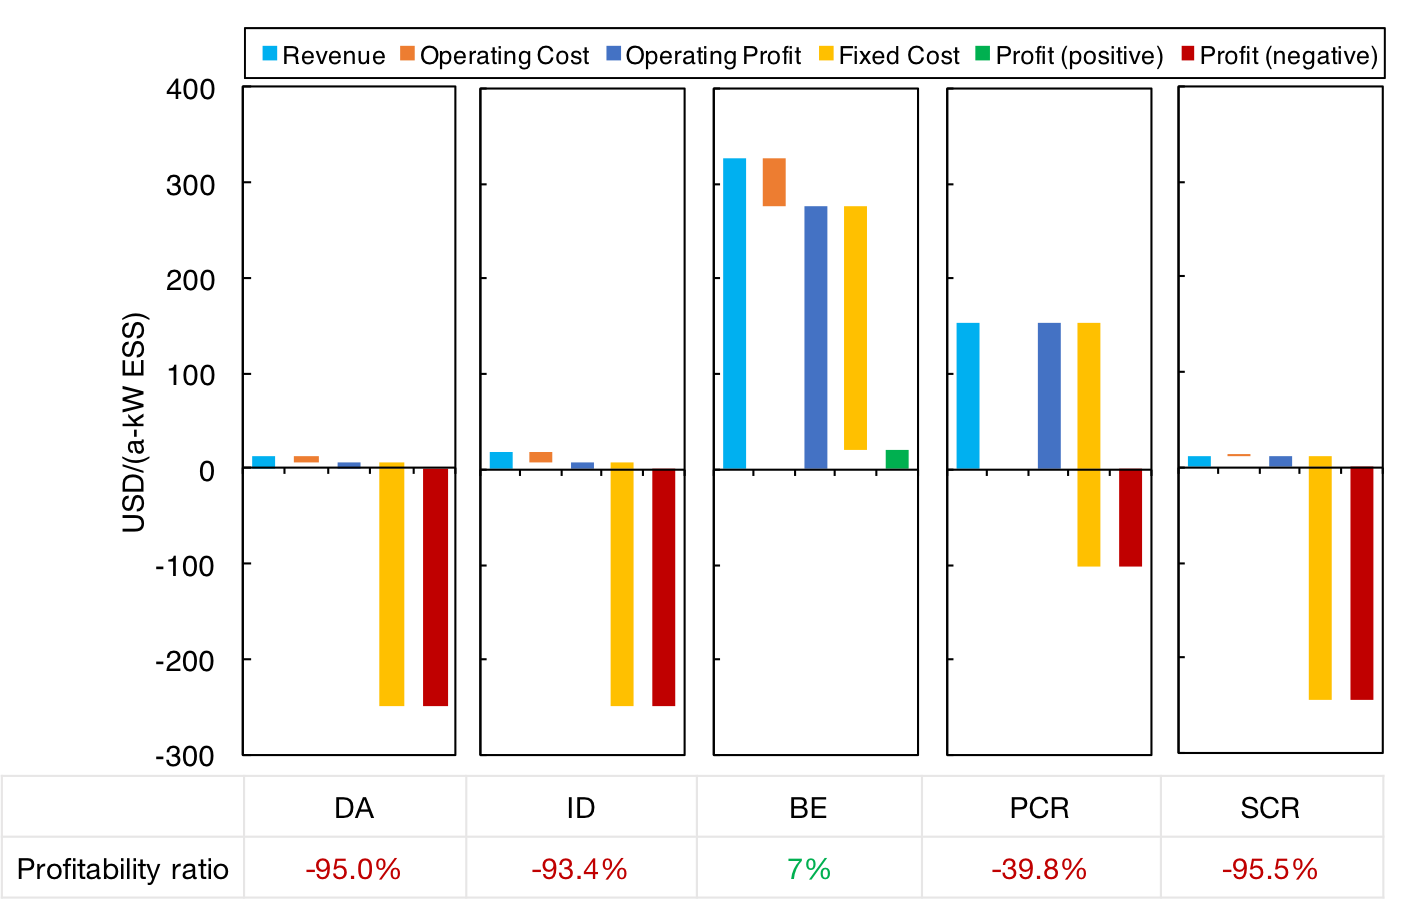
\includegraphics[width=0.9\linewidth]{Figures/Germany_ESS_profitability}
	\caption{Profitability of ESS in Germany electricity markets in the scenario of ``max. marginal Revenue"}
	\label{fig:germany-ess-profitability}
\end{figure}

\begin{figure}[h!]
	\centering
	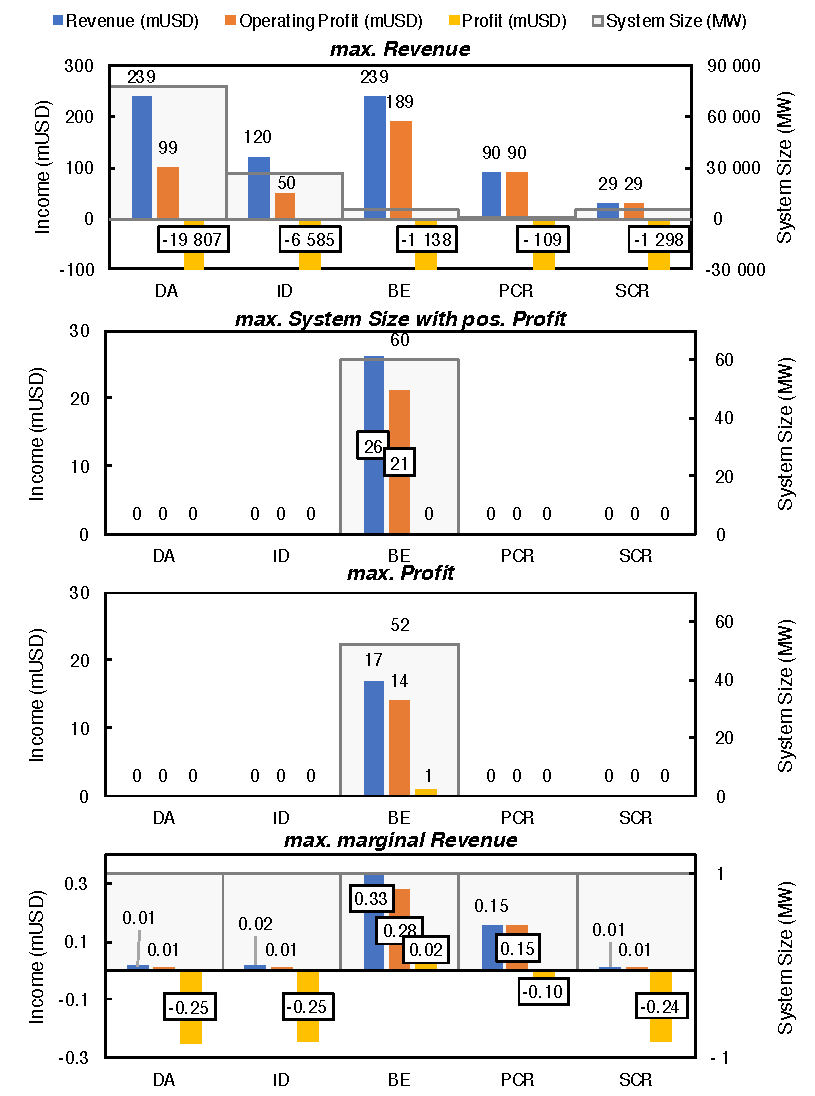
\includegraphics[width=0.9\linewidth]{Figures/Germany_ESS}
	\caption{Market size of ESS in Germany electricity markets in the scenario of ``max. Revenue"}
	\label{fig:germany-ess}
\end{figure}

As is discussed, profitability analysis can be performed using the scenario ``max. marginal Revenue", the results of which are depicted by Figure \ref{fig:germany-ess-profitability}. By showing values per unit ESS system installed, we can see the maximum unit return of ESS in Germany power markets. 

Meanwhile, with ample size of ESS, maximum potential market sizes can be derived, corresponding to the scenario ``max. Revenue".
Summarized by Figure \ref{fig:germany-ess}, annual cash flows are shown per MW consumption as normilzed values to the overal average consumption, \num{59138} MW . For example, the normalized revenue for arbitrage in day-ahead market is \num{4041} USD per year per MW consumption, which indicates the achievable revenue for a power system in Germay with 1 MW average load and corresponds to 239 mUSD/a in whole German market by mutiplying the base of \num{59138} MW.

It was found that the only profitable case is delivering balancing energy. As is analyzed in Section \ref{sec:qualitative-analysis}, this case corresponds to the situation of self-balancing where the players turn to the flexibility resource in avoidance of charges by TSOs for their imbalances. We further analyzed the maximum profitable system size and maximum profit of using the pre-defined BESSs; see Figure \ref{fig:germany-ess-profitable-size}.

\begin{figure}[h!]
	\centering
	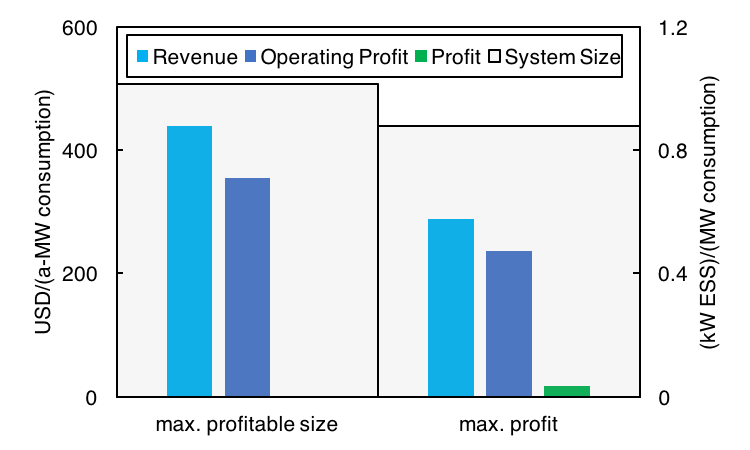
\includegraphics[width=0.9\linewidth]{Figures/Germany_ESS_profitable_size}
	\caption{Market size of ESS in Germany electricity markets in the scenario of ``max. System size with pos. Profit" and ``max. Profit"}
	\label{fig:germany-ess-profitable-size}
\end{figure}

It can be seen from Figure \ref{fig:germany-ess-profitable-size}, if being operated optimally BESSs with a size of up to 1 kW/(MW consumption) can generate profits by serving balancing energy, corresponding to a total 60MW in Germany. Nevertheless, it is challenging to be realized in practice. Market players do not have the right information to optimize their operational plans, since the balancing energy price, reBAP, is calculated \textit{ex-post} and highly volatile, hardly predictable, as is discussed in Section \ref{sec:qualitative-analysis}. On the contrary, if a system is designed to have ample size and tackle almost all imbalance events, it corresponds to a situation as the ``max. Revenue" scenario where we see negative profits from Figure \ref{fig:germany-ess-profitability}.

On the other hand, we noticed from Figure \ref{fig:germany-ess-profitability} that selling frequency control services to TSOs is less economically viable than using BESSs for self-balancing.The maximum marginal revenue from self-balance is significantly higher (33 times) than from selling frequency control products, while ideally the situation shall be reversed. The balancing energy charges are designed to recover the costs of activating frequency control services (calling for energy delivery) while the costs paid for securing capacity commitment are socialized, as have been fully discussed in Section \ref{sec:qualitative-analysis}. Theoretically, players shall get higher turnover in the frequency control markets than avoided balancing energy charges. Furthermore, the actual total payment for SCR in Germany is 176 mUSD in 2016 which is equavilent to \num{2976} USD/$(\text{a} \cdot \text{MW})$, while the maximum achievable revenue with BESSs are bounded at \num{490} USD/$(\text{a} \cdot \text{MW})$ as shown in Figure \ref{fig:germany-ess} with the rest 83.5\% of the market is intangible for BESSs . Our results imply that the current design of frequency control markets is neither economically efficient nor technically feasible to integrate the emerging BESS resources, which verifies our analysis in Section \ref{sec:qualitative-analysis}. We have argued that hurdles exist against emerging BESS to participate in frequency control markets with the non-energy-neutral signals and block-wise offering, especially for SCRs which demand significantly higher energy delivery than PCRs.

Facing either lack of information transparency in balancing energy charges or unfavorable market rules in frequency control markets, BESS players have no feasible options in the current market setup to make profits.

However, we may argue this situation shall not be long-lasting. We have already seen that certain amount of BESS will be a cheaper option to defer the expense on imbalance settlements compared to what are currently incurred. The market operators shall develop well-designed frameworks to encourage the participation of these resources that are beneficial to lower the overall system costs. In reality, there are indeed debates proposing possible solutions on this issue, e.g. letting TSOs who have the most abundance of information own and dispatch the storage resources\cite{He2012}, re-engineering the pricing mechanism of balancing energy\cite{Wartsila2014} and implementing favorable frequency control products for storage\cite{Megel2017}, etc.

As an implication for technology vendors, these possible movements on market designs shall be taken care of as it could suddenly turn over the feasibly profitability of using BESSs for balancing services.

Regarding arbitrages value in energy market, although the potential revenues are \num{4041} USD/$(\text{a} \cdot \text{MW})$ in day-ahead and \num{2029} USD/$(\text{a} \cdot \text{MW})$ in intra-day market, the losses would be incredibly high in order to materialize the revenue using BESSs; see Figure \ref{fig:germany-ess}. Even in the scenario of maximum unit return, the losses are about 10-20 times of the revenue; see Figure \ref{fig:germany-ess-profitability}. It is clear that the heavy investments on batteries cannot be recovered from making arbitrage in energy market. However, since the operating profits are always positive, if technology vendors can enable similar functions as BESS using technologies with smaller capital costs such as certain types of DR, it is still possible to make profits out of the market worth a total of over 300 mUSD per annum in Germany.

\begin{figure}[h!]
	\centering
	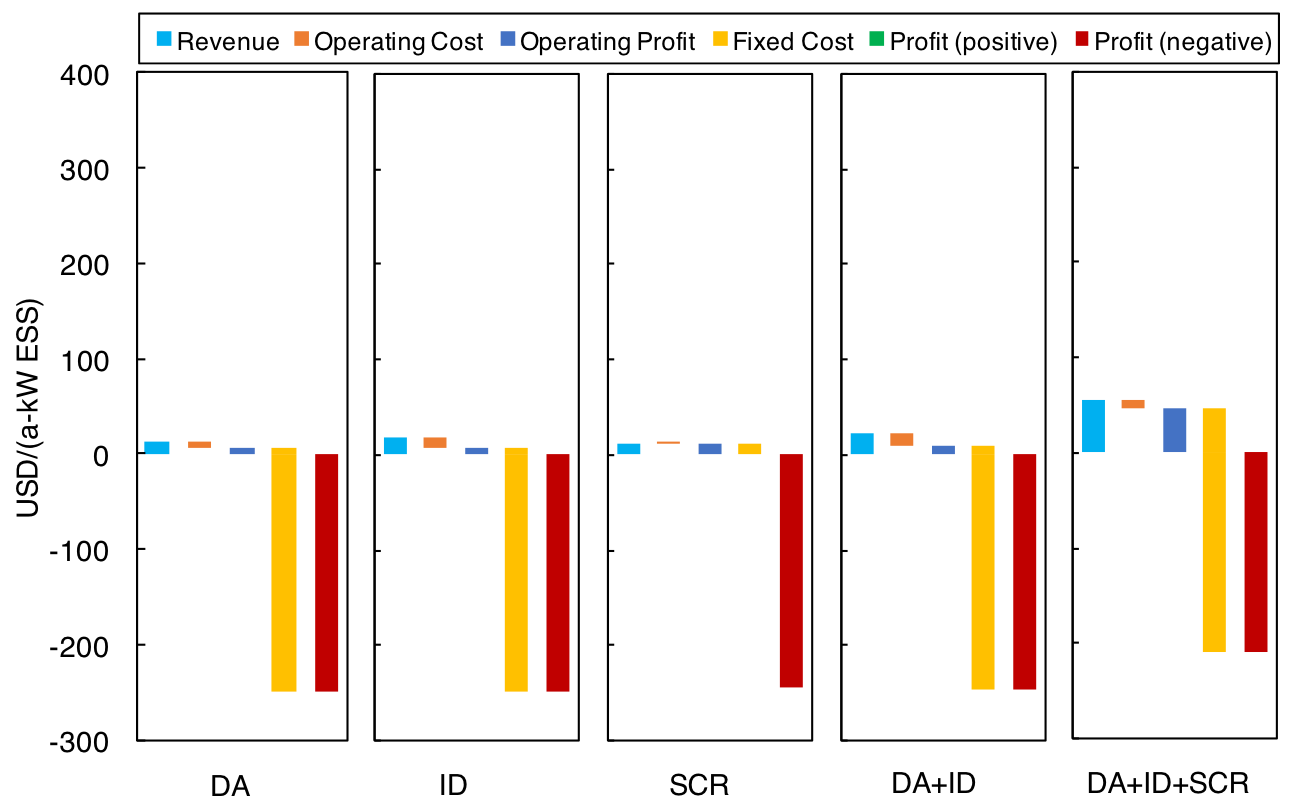
\includegraphics[width=0.95\linewidth]{Figures/Germany_ESS_profitability_multitasking}
	\caption{Profitability of ESS with multitasking in Germany electricity markets}
	\label{fig:germany-ess-multitasking-profitability}
\end{figure}

\begin{figure}[h!]
	\centering
	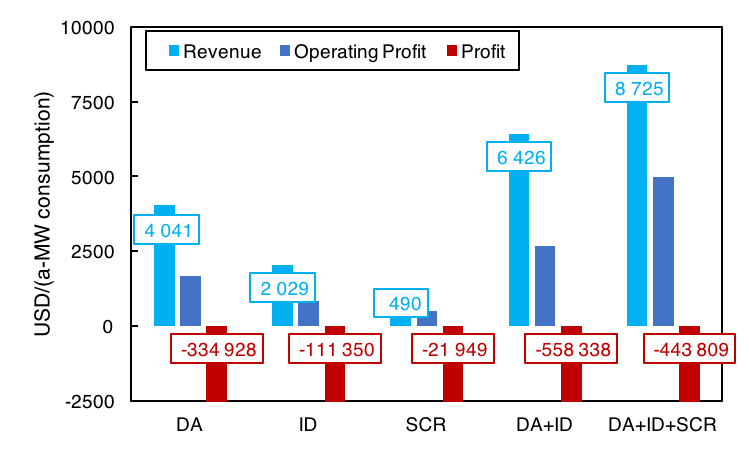
\includegraphics[width=0.95\linewidth]{Figures/Germany_ESS_multitasking}
	\caption{Market size of ESS with multitasking in Germany electricity markets}
	\label{fig:germany-ess-multitasking}
\end{figure}

As has been discussed qualitatively, in order to increase the profitability and find a way to neutralize the frequency control signals, we may stack operations in day-ahead, intra-day and secondary control reserve for multitasking. Figure \ref{fig:germany-ess-multitasking} shows the effects of multitasking.

While there are no significant synergies observed between day-ahead and intra-day markets (the unit returns remain unchanged in the scenario of maximum marginal revenue), stacking secondary control reserve with these two energy marketplaces will significantly improve the unit revenue (from 11 and 22 USD/$(\text{a} \cdot \text{MW})$ to 54 USD/$(\text{a} \cdot \text{MW})$) as well as the maximum revenue potential (from \num{6426} USD/$(\text{a} \cdot \text{MW})$ plus \num{490} USD/$(\text{a} \cdot \text{MW})$ to \num{8725} USD/$(\text{a} \cdot \text{MW})$). The maximum unit operating profit, as a consequence, raises by 4.5 times. The increment of maximum potential revenue of \num{2299} USD/$(\text{a} \cdot \text{MW})$ by stacking SCR on DA+ID indicates an additional revenue of \num{1809} USD/$(\text{a} \cdot \text{MW})$ are accessible for ESS in the SCR markets, reducing the intangible part from 83.5\% to 22.7\%. This corresponds to our previous analysis that the non-energy-neutral signal is indeed an issue for BESSs and has to be neutralized externally. Nonetheless, coping with third-party energy transactions requires the BESSs spare certain capacity to receive or release the energy, which reduces their availability in delivering SCR services. This is reflected on the result that this case with multitasking is still not profitable.

To sum up, while arbitrage is mainly constrained by costs on the technology side, making profits from balancing services is limited by adverse market frameworks although it has already shown its ability to make a positive contribution to the system. Technology vendors shall consider other technologies than BESSs or expect drastic cost reduction of BESSs to unlock the arbitrage value worth over a total of 300 mUSD/a in Germany. Profits from balancing market are more technically tangible, yet adjustments on market frameworks are required.

\subsubsection{ESS in PJM: successful practice of frequency control product design for flexibility}
The results of case studies in PJM power markets are illustrated in Figure \ref{fig:pjm-ess-profitability} and Figure \ref{fig:pjm-ess}.

\begin{figure}[h!]
	\centering
	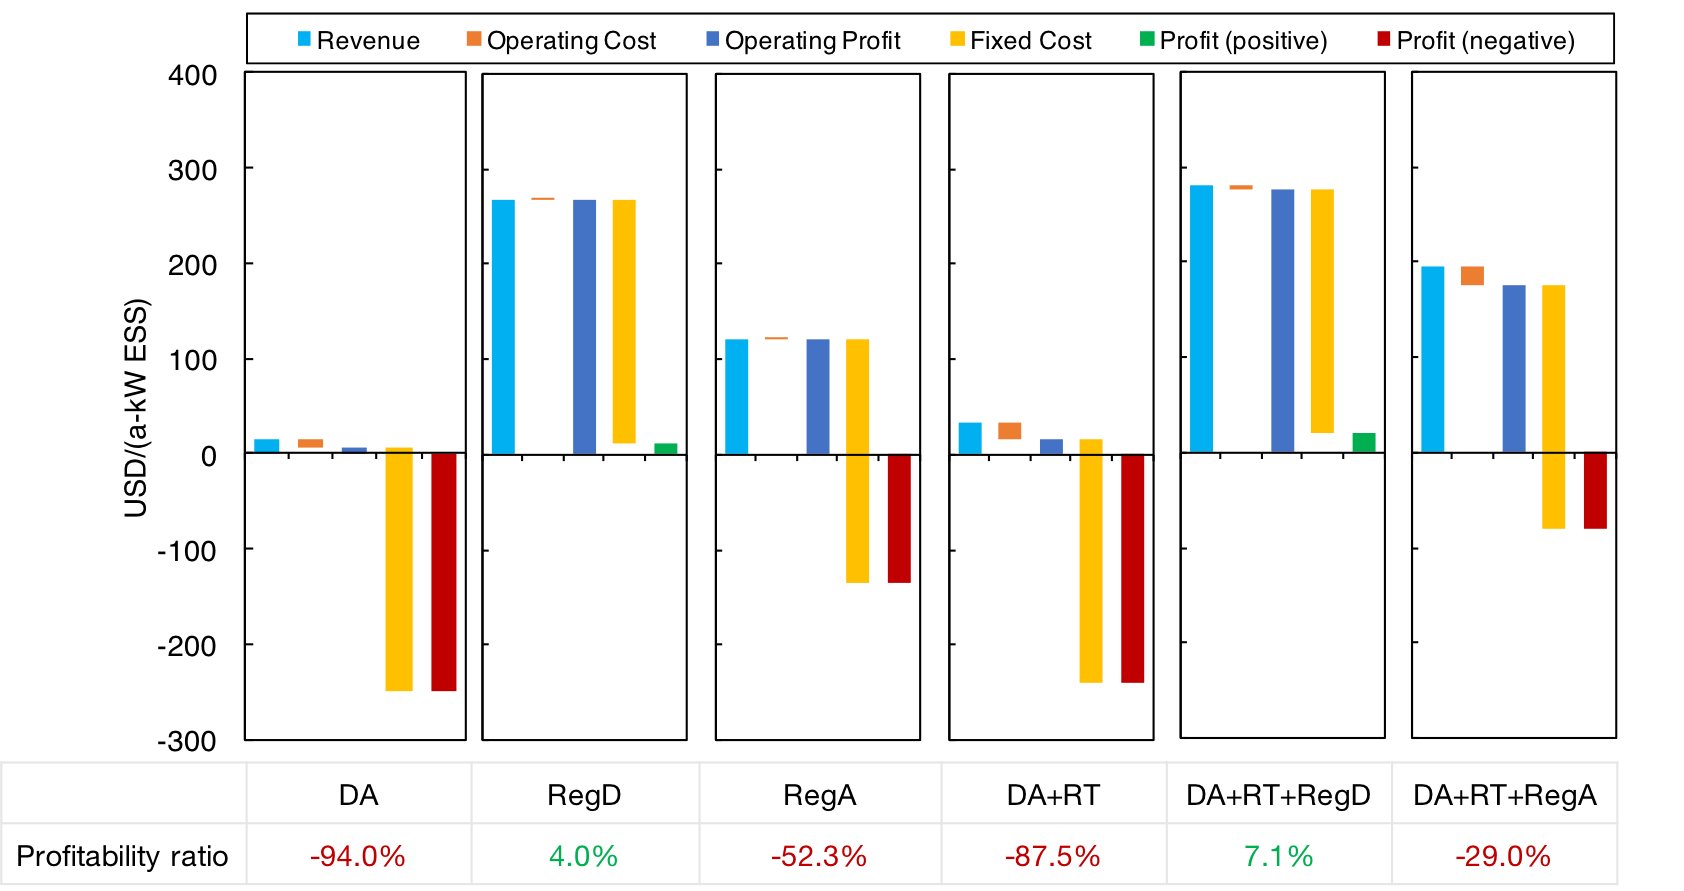
\includegraphics[width=0.9\linewidth]{Figures/PJM_ESS_profitability}
	\caption{Profitability of ESS in PJM electricity markets in the scenario of ``max. marginal Revenue"}
	\label{fig:pjm-ess-profitability}
\end{figure}

\begin{figure}[h!]
	\centering
	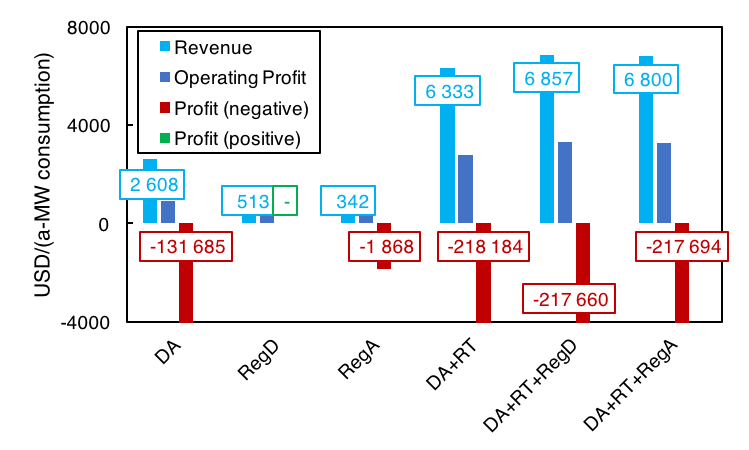
\includegraphics[width=0.9\linewidth]{Figures/PJM_ESS}
	\caption{Market size of ESS in PJM electricity markets in the scenario of ``max. Revenue"}
	\label{fig:pjm-ess}
\end{figure}

As we can clearly see, the RegD marketplace that is specially designed for emerging flexible technologies is indeed profitable. This shall give merit to PJM's RegD design including the conditional signal neutrality, operational flexibility, and higher price as a result of introducing mileage ratio and beneficial factor, as have sufficiently discussed in Section \ref{sec:qualitative-analysis}; also refer to Appendix \ref{sec:accounting-data-prepare}. The market with a total size of 513 USD/$(\text{a} \cdot \text{MW})$ can be wholly materialized by 2 kW/(MW consumption) BESSs without writing a loss, although the margin is very niche, barely above zero; see Figure \ref{fig:pjm-ess-profitable-size}.

\begin{figure}[h!]
	\centering
	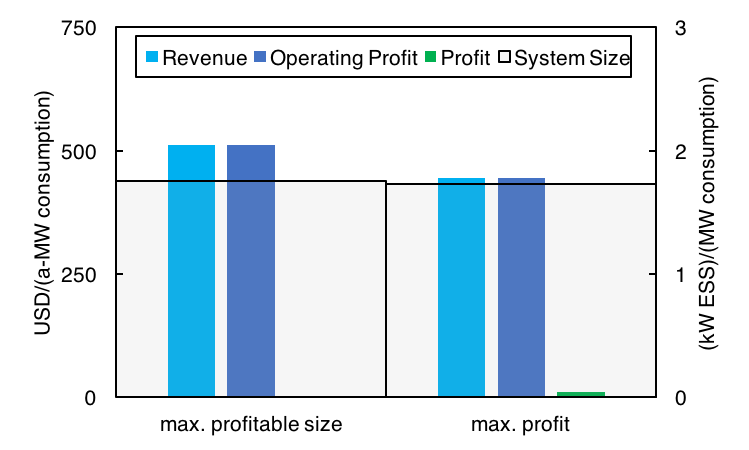
\includegraphics[width=0.9\linewidth]{Figures/PJM_ESS_profitable_size}
	\caption{Market size of ESS in PJM electricity markets in the scenario of ``max. System size with pos. Profit" and ``max. Profit"}
	\label{fig:pjm-ess-profitable-size}
\end{figure}

Those merits allow BESS players to offer RegD alone without coupled operations in the energy market which is currently necessary in Germany's power markets. As a result, stacking it with the energy market does not improve the profitability and tangible market size as significantly as in Germany. As we can see from an example shown by Figure \ref{fig:pjm-multitasking}, the system with pre-defined parameters in this study will have slightly surplus energy while strictly following the RegD signal. The SoC would raise quite slowly so that the resource can sustain the provision of RegD service over a long period (at least 84 hours shown in the chart) without involving transactions in energy markets. Trading in energy market is activated to leverage the arbitrage potential due to extreme price movements, which is however infrequent. Serving RegD is preferred for most of the time due its higher profitability. 

\begin{figure}[h!]
	\centering
	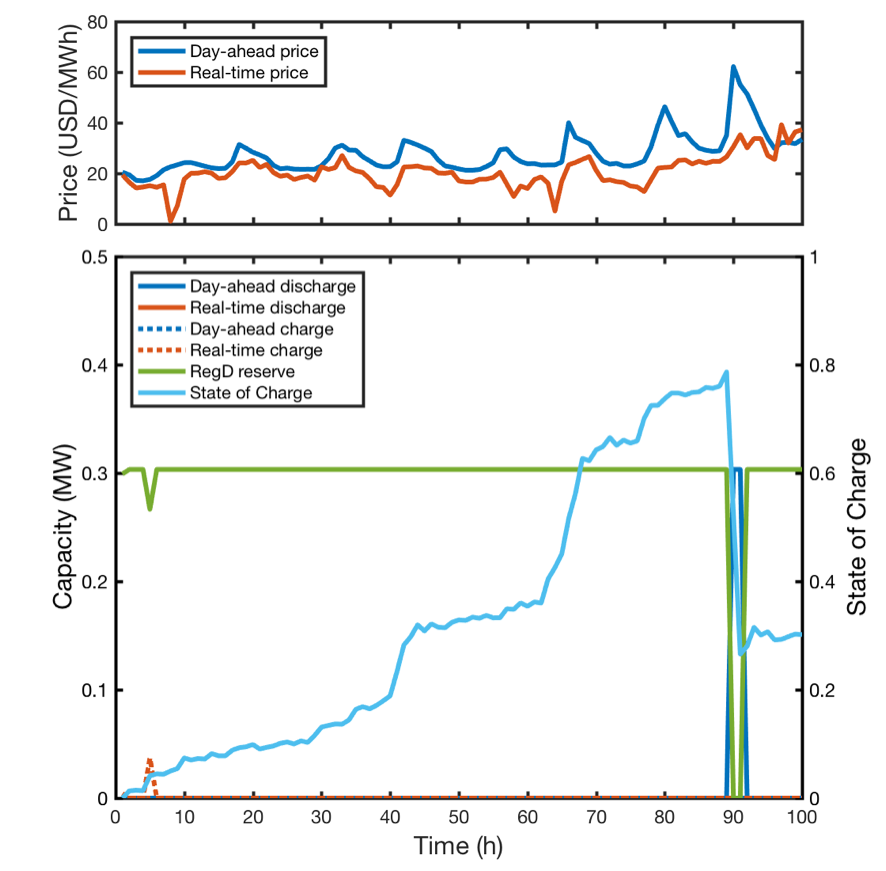
\includegraphics[width=0.9\linewidth]{Figures/PJM_multitasking_example}
	\caption{A example of operational plan with a 0.3MW battery energy storage system}
	\label{fig:pjm-multitasking}
\end{figure}

Apart from RegD market, there are no other profiting opportunities existing in PJM. Even the conventional regulation service RegA will create losses to BESS players.

Arbitrage in the energy market with flexibility through the so-called economic DR program, as is discussed in Section \ref{sec:qualitative-analysis}, is deemed not an ideal choice, especially in recent years when the electricity prices had fallen drastically with the shell gas revolution. As is discussed in Section \ref{sec:qualitative-analysis}, participating in the emergency DR program is a better option. However, the involvement of capacity market is not within our scope of quantifying the value, but the profiting mechanism is straightforward as is fully explained in the qualitative analysis. %It is also worthwhile to note that coupled operation in real-time and day-ahead markets will push the maximum revenue potential by 327 mUSD/a compared to 229 mUSD/a with participation in day-ahead market only.  

Overall, PJM shows a perfect example on how to offer incentives for the emerging storage technologies that are beneficial to the system, by implementing proper market frameworks such as the RegD and the  emergency DR program. For technology vendors, this market is already quite mature without spare space for new entrants unless significant changes may occur on market conditions, e.g. vast renewable penetration. Nonetheless, existing business cases in PJM may offer viable references for technology vendors to conduct similar practices in other markets. 
The upper-bounded values indicating the market potential are summarized in Table \ref{tab:pjm-summary}.


\subsubsection{ESS in NSW: most favorable market for arbitrage using flexibity yet still not profitable}

In New South Wales power markets, we only studied the real-time energy market, which was primarily due to the limitation of data availability.  Only information about total payment are available for the frequency control products. However, it was found that the overall size of these unaddressed markets are indeed negilible compared to the real-time energy market. The total payment in NSW's frequency control ancillary service (FCAS) market was worth 23.4 mUSD (2933 USD/$(\text{a} \cdot \text{MW})$) in 2016, which was equal to just 0.53\% of the total payment in the real-time energy market that was 4.4 bUSD (\num{551516} USD/$(\text{a} \cdot \text{MW})$). It was also much smaller than merely the arbitrage value, being 2.7\% of the revenue from arbitrage of \num{109301} USD/$(\text{a} \cdot \text{MW})$ as shown by Figure \ref{fig:nsw-ess}. This reflects the philosophy of market design to fully exploit the ability of real-time energy market to response to the system imbalances which are otherwise tackled by frequency control markets\cite{AEMO2010}\cite{McConnell2015}.
As a result, the price volatility in NSW's real-time energy market is significantly higher than the energy markets in other geographies, as is shown by Table \ref{tab:price-3-geo}.

\begin{table}[h!]
	\centering
	\begin{tabular}{l l R{3cm} R{4.5cm}}
		\hline
		\textbf{Geography} & \textbf{Market} & \textbf{Average price (USD/MWh)} & \textbf{Standard deviation of price (USD/MWh)} \\
		\hline
		NSW  & RT & 46.0 & 86.0 \\
		\hline
		\multirow{2}{*}{Germany} & DA & 34.8 & 15.0 \\
		\multirow{2}{*}{} & RT & 35.1 & 16.1 \\
		\hline
		\multirow{2}{*}{PJM} & DA & 30.0 & 11.6 \\
		\multirow{2}{*}{} & RT & 27.6 & 14.8 \\
		\hline
	\end{tabular}
\caption{The average and standard deviation of energy price in three geographies}\label{tab:price-3-geo}
\end{table}

\begin{figure}[h!]
	\centering
	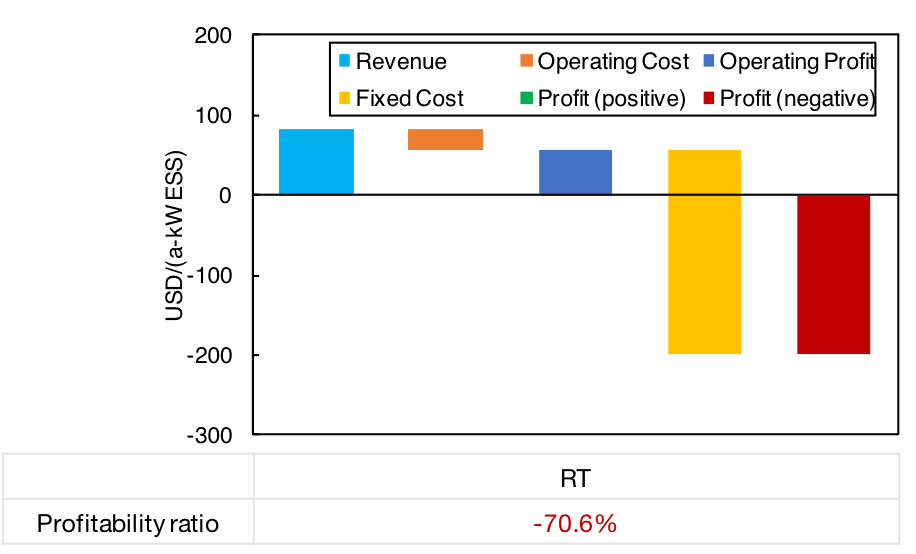
\includegraphics[width=0.9\linewidth]{Figures/NSW_ESS_profitability}
	\caption{Profitability of ESS in NSW electricity markets in the scenario of ``max. marginal Revenue"}
	\label{fig:nsw-ess-profitability}
\end{figure}

\begin{figure}[h!]
	\centering
	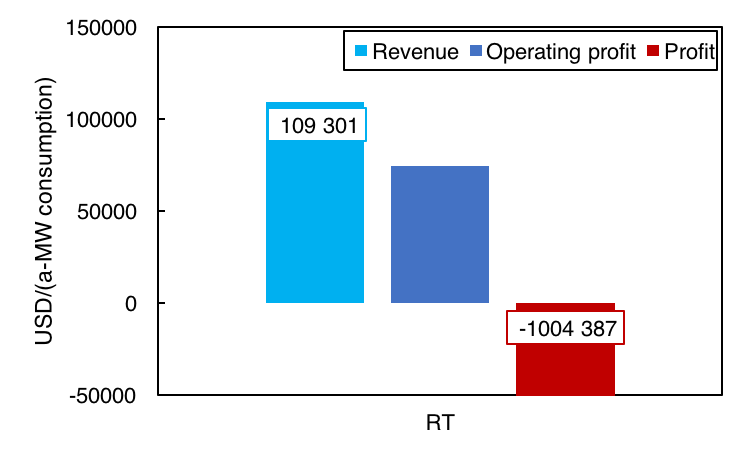
\includegraphics[width=0.9\linewidth]{Figures/NSW_ESS}
	\caption{Market size of ESS in NSW electricity markets in the scenario of ``max. Revenue"}
	\label{fig:nsw-ess}
\end{figure}

Such a volatile market is favorable for arbitrage. As we can see from Figure \ref{fig:nsw-ess-profitability} and \ref{fig:nsw-ess}.Profitability-wise the marginal revenue per unit system, 83 USD/$(\text{a} \cdot \text{kW ESS})$) is 2.4 times the value of arbitrage in DA+RT in PJM and 3.8 times the value of arbitrage in DA+ID in Germany. In terms of market potential, the maximum arbitrage revenue \num{109301} USD/$(\text{a} \cdot \text{MW})$) is roughly 17 times higher compared to either of those two arbitrage cases in Germany and PJM.

Nonetheless, even though in such a voltaile real-time energy market, it is still not a profitable business to deploy BESS in NSW for arbitrage.

\subsubsection{Cost reduction: where is the break-even point for arbitrage using BESSs}
According to the results above, using BESSs for balancing is already technically feasible while limitations lie on the aspect of market design. The value of arbitrage, however, is far away from being profitable due to high expenses on batteries. Overturn of arbitrage profitability using BESSs has to rely on reducing costs and changing market conditions. While the latter will be discussed in the proceeding section, hereby we present the results with reduced costs of battery stocks. 

In each geography, the case with the highest arbitrage potential was selected, which is respectively arbitrage in coupled day-ahead and intra-day market in Germany (DA+ID), arbitrage in coupled day-ahead and real-time market in PJM (DA+RT), arbitrage in real-time market in NSW (RT). We would show the maximum profitability ratio that is realized by a small size of BESS. Meanwhile  we would present the profitable revenue that is obtained as in the scenario of ``max. System Size with pos. Profit" to the maximum potential revenue derived from the scenario ``max. Revenue". It shall be pointed out the maximum revenue that is independent from costs would remain constant so adopted as the cardinal term to illustrate the growth of profitability. 

\begin{figure}[h!]
	\centering
	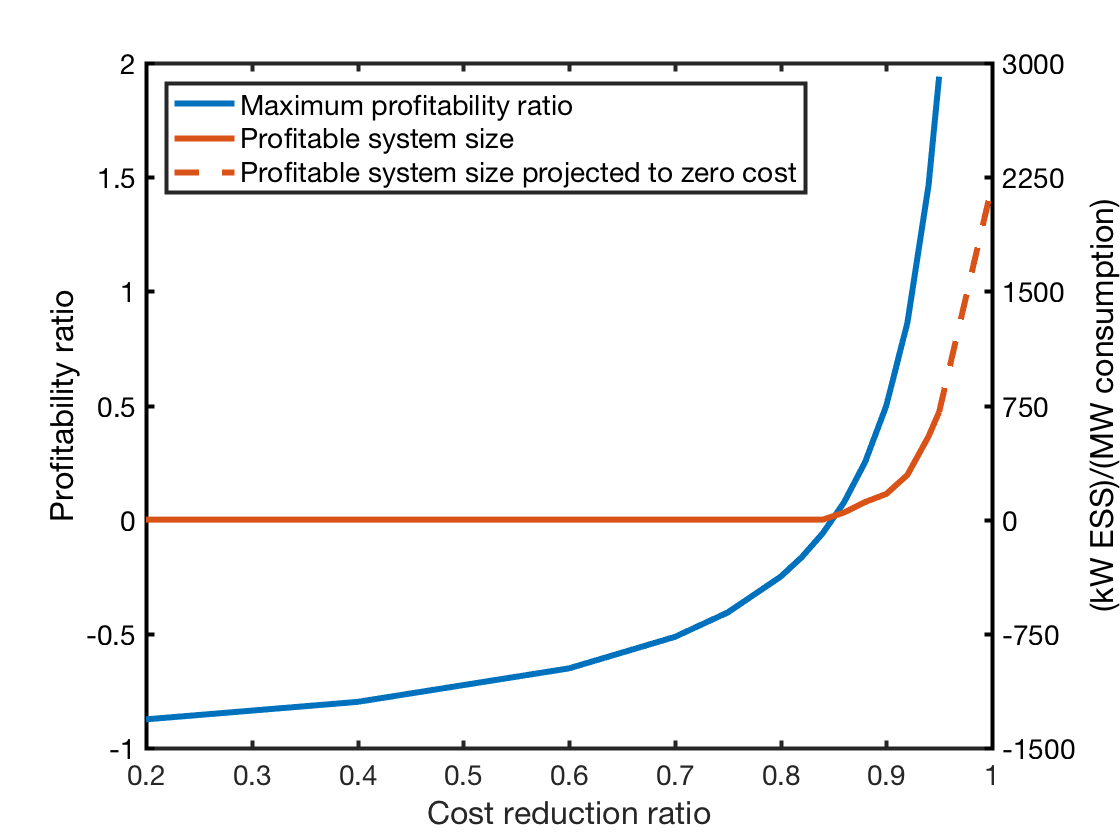
\includegraphics[width=0.9\linewidth]{Figures/CostReduction_Germany_ESS}
	\caption{Development of market size and profitability of arbitrage in coupled day-ahead and intra-day markets with reduced costs in Germany}
	\label{fig:germany-ess-costreduction}
\end{figure}

\begin{figure}[h!]
	\centering
	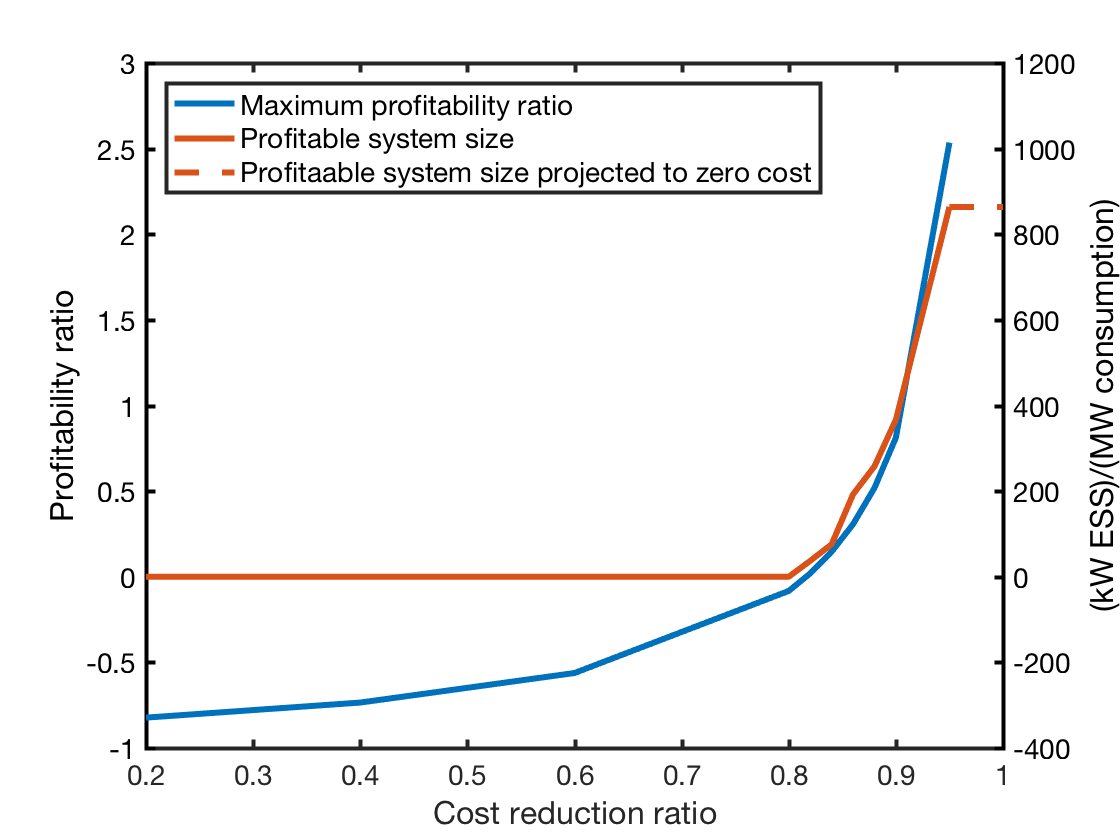
\includegraphics[width=0.9\linewidth]{Figures/CostReduction_PJM_ESS}
	\caption{Development of market size and profitability of arbitrage in coupled day-ahead and real-time markets with reduced costs in PJM}
	\label{fig:pjm-ess-costreduction}
\end{figure}

\begin{figure}[h!]
	\centering
	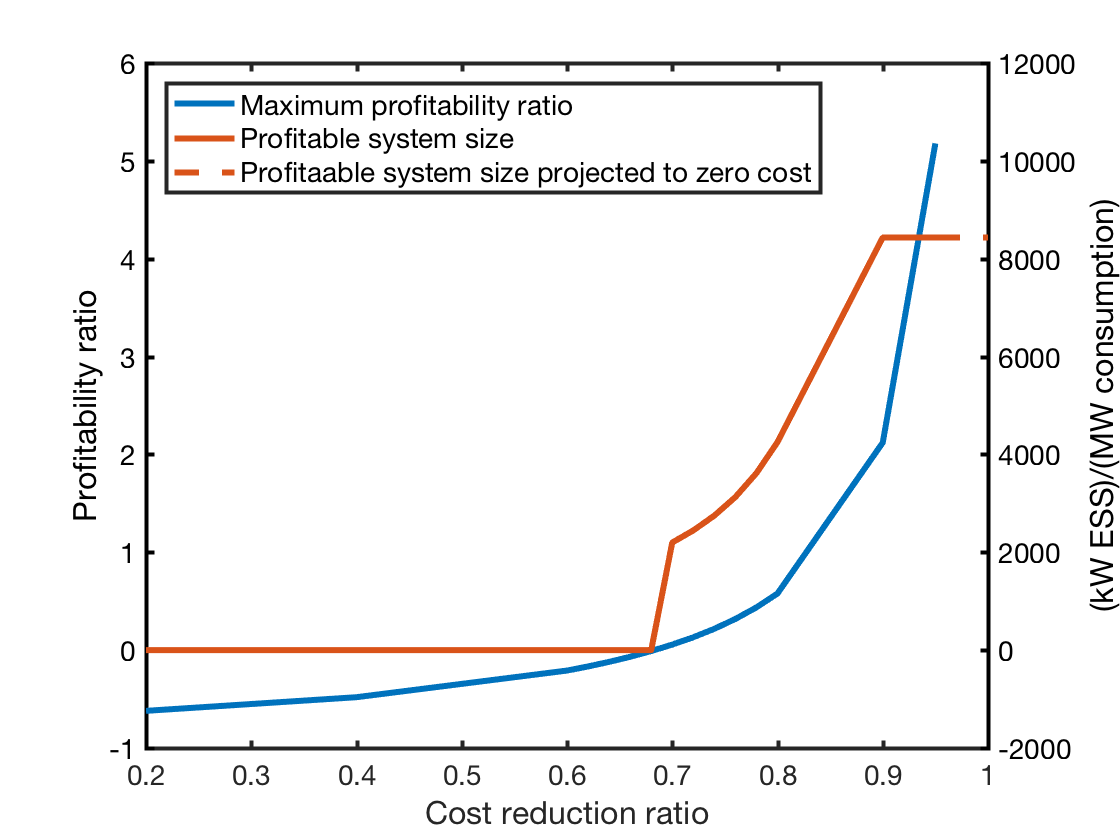
\includegraphics[width=0.9\linewidth]{Figures/CostReduction_NSW_ESS}
	\caption{Development of market size and profitability of arbitrage in real-time markets with reduced costs in NSW}
	\label{fig:nsw-ess-costreduction}
\end{figure}

Figure \ref{fig:germany-ess-costreduction} - \ref{fig:nsw-ess-costreduction} illustrate how the profitability and market size will evolve with cost reduced by up to 95\% in three geographies. The break-even point of costs is found to be 84\%, 81\% and 68\%, respectively in Germany, PJM and NSW. If we adopt the forecast made by IRENA\cite{IRENA2017} who predict the cost reduction by up to 60\% by 2030, none of these markets will be profitable for arbitrage by 2030. Even if we applied a constant learning rate of 14\% per annum according to \cite{Nykvist2015}, the break-even point will be realized in 12, 11 and 8 years, respectively in Germany, PJM and NSW. 

Moreover, it shall be noticed while the break-even point is just reached, the total profitable revenue will be almost at zero. To materialize the whole potential of arbitrage revenue, it requires a cost reduction of 95\%+, 95\% and 90\%, respectively in Germany, PJM and NSW, which is almost impossible to be realized in the foreseeable future.

As a conclusion, the cost reduction of BESS by learning effect alone will not turn over the profitability of arbitrage using BESSs in the near future. Unless revolutionary technical innovations happen, opportunities of arbitrage using BESS may only arise with drivers from the market, e.g. renewable penetrations, which are to be shown in Section \ref{sec:impact-market-condition}.

\subsubsection{EV2G  in Germany: changeling in developing business model}
Implementing EV as a grid resource is not as straightforward as using generic ESSs that is discussed above. The main issue is that the energy demand for EV driving itself poses challenges to grid. It is not possible to deliver any services without incorporate a large-volume energy market. Therefore, the day-ahead energy market is always included for all the cases for EV2G. Moreover, in our case studies, it is found even with the day-ahead market, charging the EVs is not feasible while their number reached a certain level. In the optimization framework, the technology constraints would violate market constraints, especially the one that we set to restrict the activation of peak generation during non-peak hours, while the EV fleet grows beyond a certain scale. This corresponds to the situation where spare generation resources in the power system are not sufficient  to fulfill the energy needs of EVs. The electricity price may raise significantly in those scenarios compared to nowadays's level. As is shown by Figure \ref{fig:EV_nan_percentageg}, when the number of EV is higher than 1 million, it start to stress the electricity supply if the generation capacity remains at present level. 
\begin{figure}[h!]
	\centering
	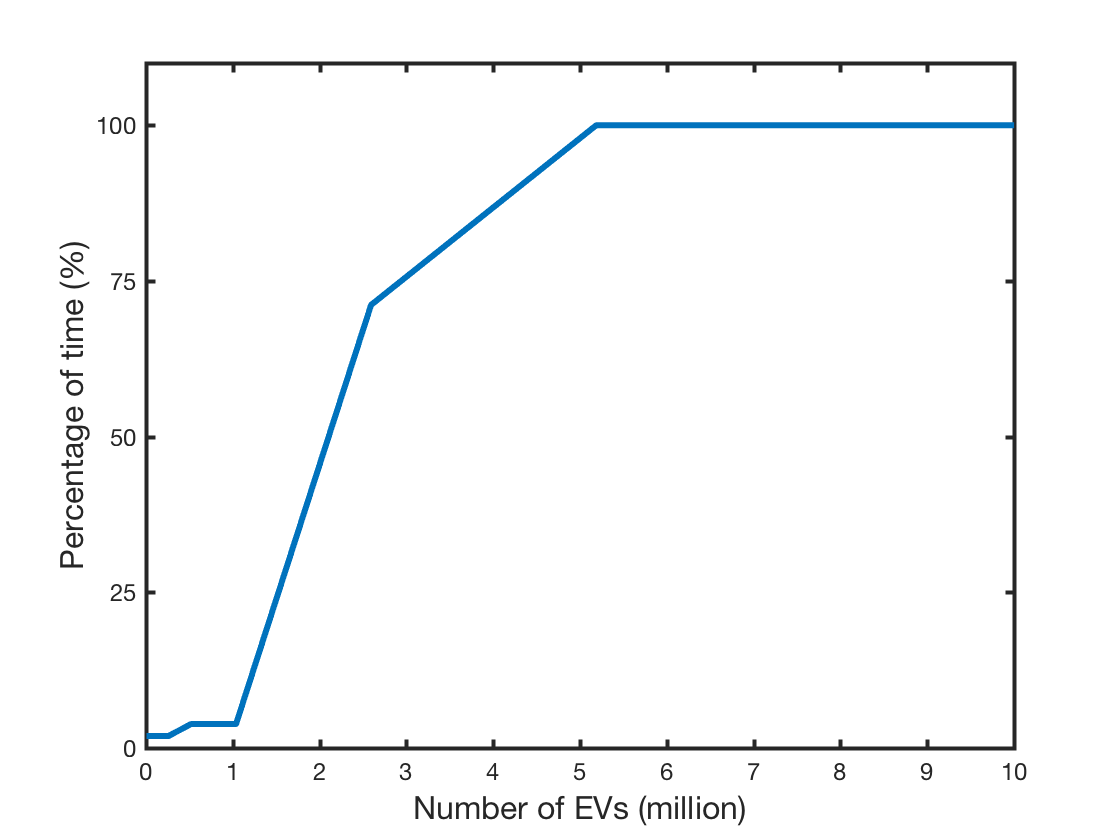
\includegraphics[width=0.95\linewidth]{Figures/EV_nan_percentage}
	\caption{Percentage of time when EV charging demand cannot be fulfilled in Germany}
	\label{fig:EV_nan_percentageg}
\end{figure}

This finding implies when there will be 1 million more EVs in Germany compared to the number in 2016, it will create great incentives for infrastructure extension of electricity grid, which reveals a promising business opportunity. Nevertheless, studies under that condition is beyond the focus of our work. Instead, we would only perform scenario analysis when the number of EV is within the limit of 1 million. 

In this thesis, we applied three scenarios studying the EV2G market in Germany:

\begin{itemize}
	\item \textbf{EV number 2016:} assuming all  EVs in Germany by 2016 are contract for delivering EV2G services
	\item \textbf{EV number 2017:} similar to the first scenario but using the data of 2017
	\item \textbf{2\% market share:} assuming EVs will account for 2\% of the total vehicle number in Germany (45 million according to \cite{Eurostat_de_v}) i.e. 0.9 million EVs in the future
\end{itemize}

According to the Federal Motor Transport Authority of Germany (Kraftfahrt-Bundesamtes, KBA)\cite{KBA2017}, the number of plug-in electric vehicles has grown fast over the past year, especially in 2017. Since the EV registered before 2010 is negligible, we conceived the cumulative registration since 2010 as the total number of EVs in Germany, shown as Figure \ref{fig:Germany_EV_number}.

\begin{figure}[h!]
	\centering
	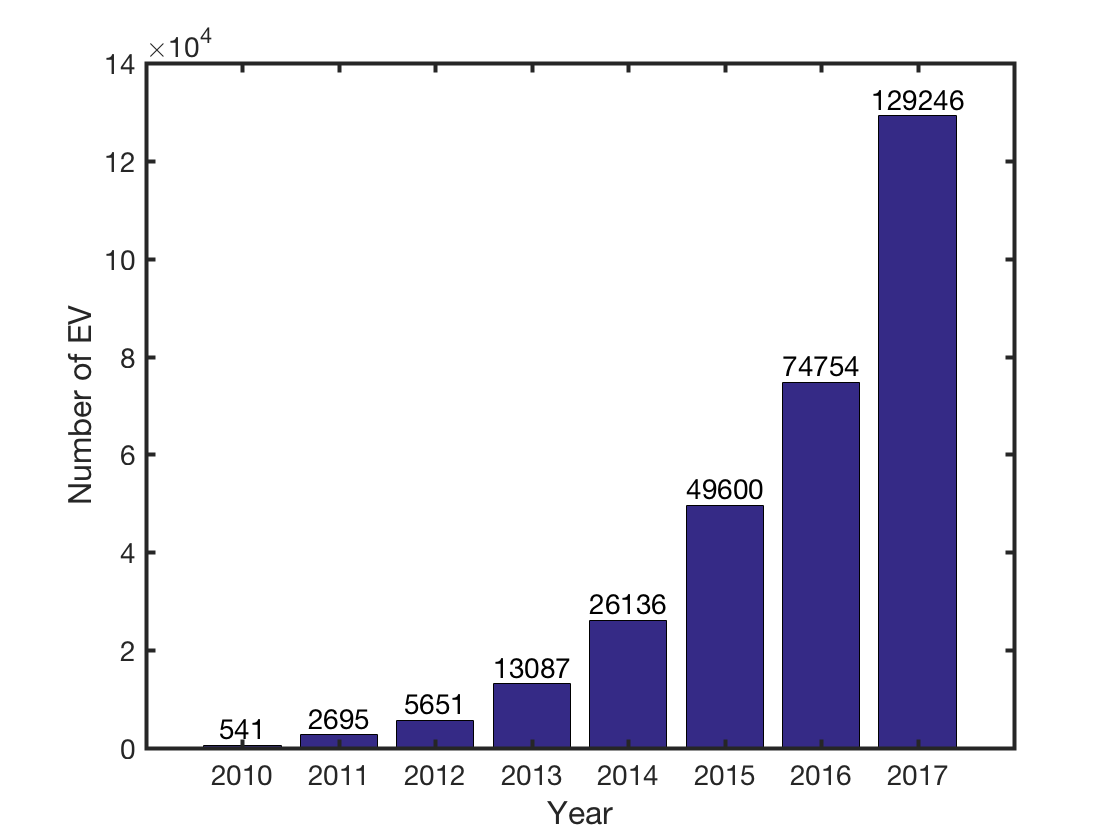
\includegraphics[width=0.95\linewidth]{Figures/Germany_EV_number}
	\caption{Cumulative registration of plug-in electric vehicles in Germany since 2010 \cite{KBA2017}}
	\label{fig:Germany_EV_number}
\end{figure}

The numbers of EV that were taken for the scenario analysis are then determined and list in Table \ref{tab:ev-number-scenario-germany}.

\begin{table}[h!]
	\centering
	\begin{tabular}{l r r}
		\hline
		\textbf{Scenario} & \textbf{EV number total} & \textbf{EV number per household} \\
		%\hline
		\hline
		EV number 2016 &  \num{74754} & \num{0.014} \\
		EV number 2017 &  \num{129246} & \num{0.025} \\
		2\% market share &  \num{900000} & \num{0.174} \\
		\hline
	\end{tabular}
\caption{The number of EV for each scenario in Germany}\label{tab:ev-number-scenario-germany}
\end{table}

\begin{figure}[h!]
	\centering
	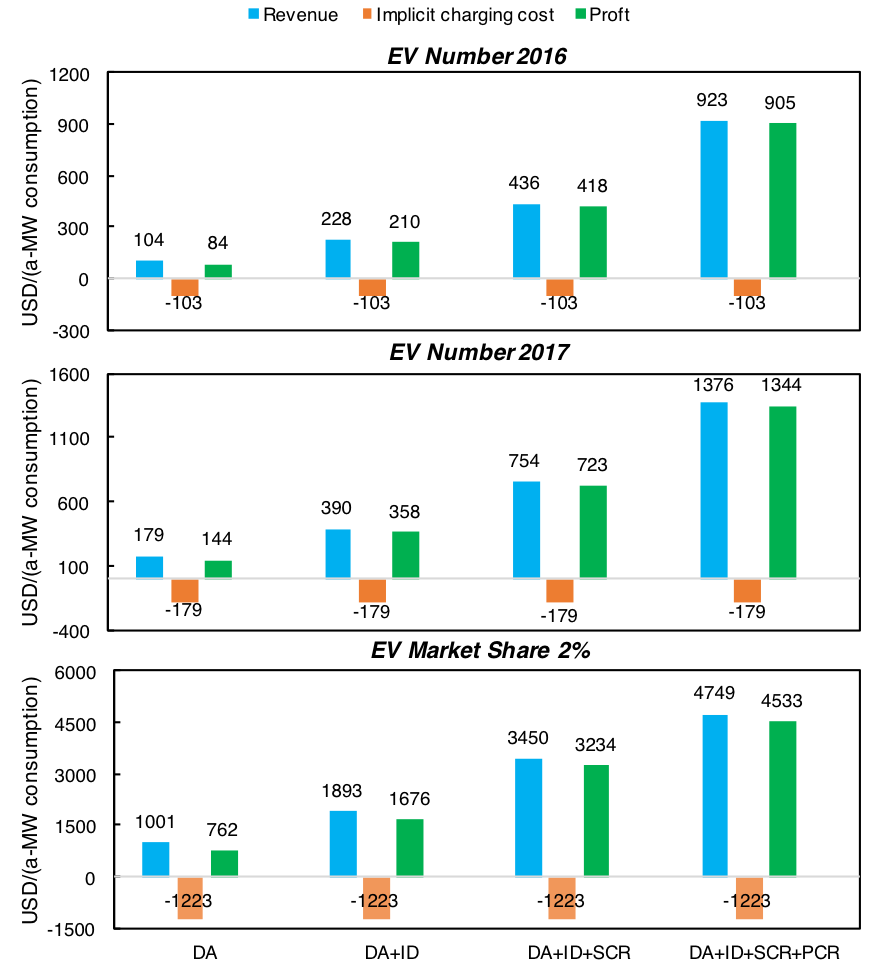
\includegraphics[width=0.95\linewidth]{Figures/Germany_EV_profit}
	\caption{Market size and profitability of EV2G in Germany electricity markets}
	\label{fig:Germany_EV}
\end{figure}

Based on these scenarios, we performed the case studies and the results are shown by Figure \ref{fig:Germany_EV}. It was found that the arbitrage only in day-ahead market was not profitable at all, while arbitrage in both day-ahead and intra-day market was barely able to maintain a revenue-cost balance. The revenues captured from arbitrage was at most compensating the cost of EV charging. Profits would be possible if a business model where services providers could charge service fees from the end-users (EV owners). Although the service fees can be much lower than the normal charging costs for the end-consumers, it would be still challenging in practice to implement such a business model because the charging cost become implicitly embedded when a EV was used for V2G services. Overall, the low arbitrage values in Germany's energy market makes these business cases not appealing. 

Coupling frequency control markets increases indeed the profits and it was found to be more promising with the drastic of EVs as there are still much more growth space till the scenario of 2\% EV market share. However, it shall be noticed that our analysis has overlooked some factors which could make the business less profitable as shown here. The main issue is that we use a determinate approach to simulate the frequency control signal and EV driving behaviors which eliminated the risks of failing to deliver the frequency control services as planned. Alipour \textit{et. al.}\cite{Alipour2017} made a study on EV2G for frequency control services with a stochastic approach. It was found in a case where a profit of 7980 USD was expected, the conditional value-at-risk was 5720 USD, indicating the risking nature of such a business. In the outlook of this thesis, we proposed a stochastic method by using Markov chain to simulate the uncertain driving behavior of EVs and then the estimation of risk can be conducted. Nonetheless, while quantitative risk assessment against uncertainty is necessary for designing a specific project, it is beyond the focus of a study understanding the whole market value so is not included in our study. Besides, implementing EV2G for frequency control is not a mature technology due to its complexity\cite{Peng2017}\cite{Shafie-Khah2015}\cite{Bessa2014}\cite{Bessa2013}, which implies a high research and development cost.

It is also worthwhile to note that while the number of EVs (0.9 million ) in the scenario of ``2\% Market Share" has reached the edge of the affordable level (1 million) for the grid, revenues are significantly smaller than the maximum potential revenues derived in the case studies of ESSs. The shares of maximum achievable revenue by EV2G to the total market potential by generic ESS were between 18-37\% among different cases. This reveals that constrained by the limitations discussed above, EV2G will not be able fully cover the needs for flexibility by its own, even on a aggregated system level without considering the distributed manners. Other types of flexibility would still be necessary to complement the demands for flexibility in scenarios with high EV penetrations.

\subsubsection{EV2G  in PJM: RegD market would be saturated shortly if EV2G was indeed implemented}

\begin{figure}[h!]
	\centering
	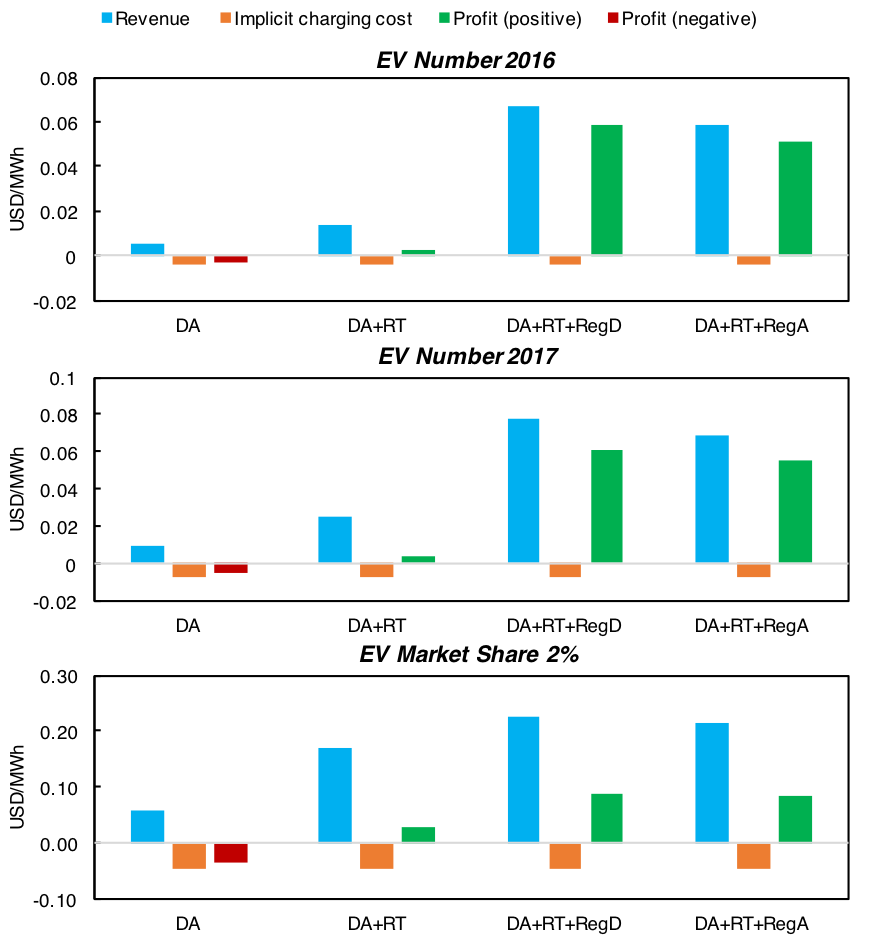
\includegraphics[width=0.95\linewidth]{Figures/PJM_EV_profit}
	\caption{Market size and profitability of EV2G in PJM Electricity markets}
	\label{fig:PJM_EV}
\end{figure}

Similar studies are performed in PJM power markets. Since the geographic coverage of PJM is not strictly corresponding to the administrative divisions, it becomes a extremely sophisticated task to get the official number of EVs in PJM with the public data. Therefore, we projected the number in Germany to PJM by their ratio of household number. That means, in the corresponding scenarios, the EV ownership per household is identical in Germany and PJM. We took this approach to make an indication of the market value, which however shall be noticed with caution that it may deviate from real conditions. 
Table \ref{tab:ev-number-scenario-PJM} shows the number of EV in each scenario.

\begin{table}
	\centering
	\begin{tabular}{ l r r }
		\hline
		\textbf{Scenario} & \textbf{EV number total} & \textbf{EV number per household} \\
		%\hline
		\hline
		EV number 2016 &  \num{43713} & \num{0.014} \\
		EV number 2017 &  \num{75578} & \num{0.025} \\
		2\% market share &  \num{526290} & \num{0.174} \\
		\hline
	\end{tabular}
	\caption{The number of EV for each scenario in PJM}\label{tab:ev-number-scenario-PJM}
\end{table}

With these numbers of EV, no generation shortage was observed, expect for only one week in the scenario of 2\% EV market share. The results in that week were discarded, i.e. no operations and thus no revenues in that week. This accounts for approximately 2\% of the time in a year so the impact on final results shall be negligible.

Figure \ref{fig:PJM_EV} summarizes the results of cases in PJM. Arbitrage in day-ahead market only was still not profitable. Coupled operations in real-time market lead to niche profits while the EV numbers are relative small, which is similar to the situation in Germany. However, with a 2\% EV market share, we saw a profit from business case while it incurred loss in Germany's DA+ID markets. This can be explained by the PJM's real-time market as a hub for all real-time settlements has much higher liquidity than the intra-day exchange in Germany.

The incremental revenue by stacking RegD to DA+RT case was 462 USD/$(\text{a} \cdot \text{MW})$ in the scenario of ``EV Number 2016" while the addtional revenue by stacking SCR to DA+ID in Germany was merely 206 USD/$(\text{a} \cdot \text{MW})$, which again reveals the favor of RegD toward flexibility resources. 

Noticing that the whole RegD market potential for generic flexiblity resources is merely 513 USD/$(\text{a} \cdot \text{MW})$ as was shown previously by \ref{fig:pjm-ess}. This market could be easily exhausted by a small size of EV fleet. 
 
\subsubsection{EV2G  in NSW: arbitrage-only is more profitable than frequency control in the other two geographies}

Using the same methodology as in PJM, scenarios are established by taking the identical EV numbers per household, as is shown by Table \ref{tab:ev-number-scenario-nsw}. With these number of EV, no supply shortage was observed.  

\begin{table}[h!]
	\centering
	\begin{tabular}{ l r r }
		\hline
		\textbf{Scenario} & \textbf{EV number total} & \textbf{EV number per household} \\
		%\hline
		\hline
		EV number 2016 &  \num{4849} & \num{0.014} \\
		EV number 2017 &  \num{8383} & \num{0.025} \\
		2\% market share &  \num{58377} & \num{0.174} \\
		\hline
	\end{tabular}
	\caption{The number of EV for each scenario in NSW}\label{tab:ev-number-scenario-nsw}
\end{table}

\begin{figure}[h!]
	\centering
	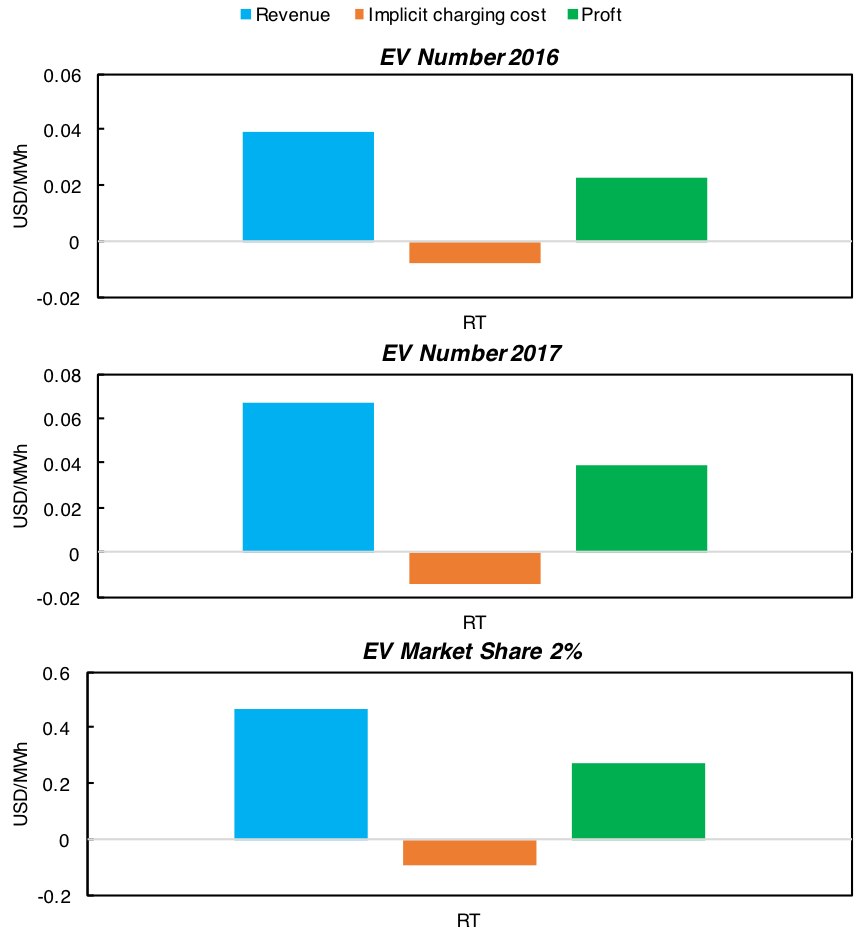
\includegraphics[width=0.95\linewidth]{Figures/NSW_EV_profit}
	\caption{Market size and profitability of EV2G in NSW Electricity markets}
	\label{fig:NSW_EV}
\end{figure}

Figure \ref{fig:NSW_EV} presents the results of three scenarios in NSW's real-time energy market. Similar to the situations in ESS cases, the market potential of arbitrage is higher than the other two geographies due to the price volatility as is cussed previously. The potential profit obtained in the scenario of ``EV Number 2016" was \num{198} USD/$(\text{a} \cdot \text{MW})$, which was 66 and 9 times the numbers in corresponding cases in Germany and PJM respectively. It is even higher than profits from business cases where frequency control are involved in other two geographies. Since arbitrage using EV is much more feasible in technology, such a high arbitrage profitability shall provide more incentives for the market participates and makes the business appealing if the number of EV will indeed grow in line with our scenarios.

Finally, it shall be noted that even in the scenario with 2\% EV market share, the market potential of arbitrage via EV2G was found to be \num{4105} USD/$(\text{a} \cdot \text{MW})$, which was just 3.8\% of the overall arbitrage potential using ample size of generic ESSs as was shown by Figure \ref{fig:nsw-ess}, leaving a vast space for other technologies.

\subsubsection{Summary}

The key indicators for the market size and profitability, in both normalized and absolute values are summarized in Table \ref{tab:germany-summary}-\ref{tab:nsw-summary}. Values were extracted at different scenarios where they are maximized. Therefore, the maximum revenue and maximum profit may not be obtained at the same time, especially for ESSs, as has been discussed at the beginning of this section.

\begin{table}
	\centering
	\begin{tabular}{l r r r r}
		\hline
		\multirow{2}{*}{\textbf{Item\footnote{Maximum values of items are obtained in different scenarios}}}& \textbf{Arbitrage} & \multicolumn{2}{c}{\textbf{Balancing}} & \textbf{Multitasking} \\
		\multirow{2}{*}{}& DA+ID & BE & FCR\footnote{Frequency control reserve, including both PCR and SCR} & DA+ID+FCR \\
		\hline
		\multicolumn{5}{l}{\textbf{Energy Storage System}} \\
		& & & & \\
		Max. Revenue [USD/$(\text{a} \cdot \text{MW})$] & \num{6426} & \num{3872} & \num{2012} & \num{10247} \\
		Max. Profit [USD/$(\text{a} \cdot \text{MW})$] & - & 17 & - & - \\
		& & & & \\
		Max. Revenue [mUSD/a] & \num{380} & \num{229} & \num{119} & \num{606} \\
		Max. Profit [mUSD/a] & - & 1 & - & - \\
		& & & & \\
		Max. Profitability Ratio & (-92\%) & 7\% & (-40\%) & (-60\%) \\
		Cost break-even\footnote{Cost reduction ratio} & (-84\%) & - &- & -\\
		& & & &\\
		\hline
		\multicolumn{5}{l}{\textbf{Electric Vehicle to Grid}} \\
		& & & & \\
		Max. Revenue [USD/$(\text{a} \cdot \text{MW})$] & \num{1961} & - & - & \num{3224} \\
		Max. Profit [USD/$(\text{a} \cdot \text{MW})$] & 8 & - & - & \num{1986} \\
		& & & & \\
		Max. Revenue [mUSD/a] & \num{116} & - & \- & \num{190} \\
		Max. Profit [mUSD/a] & \num{0.5} & - & - & 117 \\
		& & & & \\
		Max. Profit per EV [USD/(a)] & \num{4} & - & - & \num{731} \\
		& & & &\\
		\hline
	\end{tabular}
	\caption{Summary of market size and profitability of flexibility management in Germany}\label{tab:germany-summary}
\end{table}

\begin{table}
	\centering
	\begin{tabular}{l r r r r}
		\hline
		\multirow{2}{*}{\textbf{Item\footnote{Maximum values of items are obtained in different scenarios}}}& \textbf{Arbitrage} & \multicolumn{2}{c}{\textbf{Balancing}} & \textbf{Multitasking} \\
		\multirow{2}{*}{}& DA+RT & RegD & RegA & DA+RT+Reg\footnote{Including both RegD and RegA}\\
		\hline
		\multicolumn{5}{l}{\textbf{Energy Storage System}} \\
		& & & & \\
		Max. Revenue [USD/$(\text{a} \cdot \text{MW})$] & \num{6333} & \num{524} & \num{467} & \num{7324} \\
		Max. Profit [USD/$(\text{a} \cdot \text{MW})$] & 0 & 11 & 0 & 53\\
		& & & &\\
		Max. Revenue [mUSD/a] & \num{556} & \num{46} & \num{41} & \num{643}\\
		Max. Profit [mUSD/a] & 0 & 1 & 0 & 3\\
		& & & & \\
		Max. Profitability Ratio & (-88\%) & 8\% & (-29\%) & 9\%\\
		Cost break-even\footnote{Cost reduction ratio} & (-81\%) & - & - & -\\
		& & & & \\
		\hline
		\multicolumn{5}{l}{\textbf{Electric Vehicle to Grid}} \\
		& & & & \\
		Max. Revenue [USD/$(\text{a} \cdot \text{MW})$] & \num{1504} & - &  - & \num{2351}\\
		Max. Profit [USD/$(\text{a} \cdot \text{MW})$] & 261 & - & - & \num{1218} \\
		& & & & \\
		Max. Revenue [mUSD/a] & \num{132} & - &  - & \num{206}\\
		Max. Profit [mUSD/a] & \num{23} & - &  - & \num{107} \\
		& & &  & \\
		Max. Profit per EV [USD/(a)] & \num{45} & - & - &\num{1657}\\
		& & & & \\
		\hline
	\end{tabular}
	\caption{Summary of market size and profitability of flexibility management in PJM}\label{tab:pjm-summary}
\end{table}

\begin{table}
	\centering
	\begin{tabular}{l r r}
		\hline
		\multirow{2}{*}{\textbf{Item\footnote{Maximum values of items are obtained in different scenarios}}}& \textbf{Arbitrage} & \textbf{Balancing} \\
		\multirow{2}{*}{}& DA+RT & FCAS\footnote{Values based on payment on a whole system level without involving technical analysis} \\
		\hline
		\multicolumn{3}{l}{\textbf{Energy Storage System}} \\
		& & \\
		Max. Revenue [USD/$(\text{a} \cdot \text{MW})$] & \num{109301} & \num{2933} \\
		Max. Profit [USD/$(\text{a} \cdot \text{MW})$] & - & - \\
		& & \\
		Max. Revenue [mUSD/a] & \num{872} & \num{23} \\
		Max. Profit [mUSD/a] & - & - \\
		& & \\
		Max. Profitability Ratio & (-70\%) & - \\
		Cost break-even\footnote{Cost reduction ratio} & (-68\%) & \\
		& & \\
		\hline
		\multicolumn{3}{l}{\textbf{Energy Storage System}} \\
		& & \\
		Max. Revenue [USD/$(\text{a} \cdot \text{MW})$] & \num{4105} & - \\
		Max. Profit [USD/$(\text{a} \cdot \text{MW})$] & \num{2382} & - \\
		& & \\
		Max. Revenue [mUSD/a] & \num{33} & - \\
		Max. Profit [mUSD/a] & 19 & - \\
		& & \\
		Max. Profit per EV [mUSD/a]& 326 & - \\
		& & \\
		\hline
	\end{tabular}
	\caption{Summary of market size and profitability of flexibility management in NSW}\label{tab:nsw-summary}
\end{table}

\newpage
\subsection{Impact analysis of renewable penetration}
\label{sec:impact-market-condition}

As is mentioned at the beginning of this section, understanding the impact of some key factors is crucially viable to plan future business on flexibility management, as the market may evolve rapidly. Among all the factors, we have selected the renewable penetration as the most influencing factor and studied in this thesis. The rationale can be explained as the renewable penetration would change most radically compared to other factors and is viewed as the essential driver of growing needs for flexibility, which has been elaborated in Chapter \ref{ch:introduction}. 

Growing capacity of renewable generations will influence both wholesale energy and frequency control markets as we have seen from the literature; refer to Chapter \ref{ch:LitRev}. However, determining the requirement for frequency control reserve is an extremely sophisticate process of grid planning, which is rarely addressed by academic articles. Grid planner may initiated large-scale research project dealing with this problem. Referring to a study ordered by PJM and conducted by a research consortium led by GE Consulting\cite{GEEnergyConsulting2014}, an average of 1533 MW frequency regulation reserve would be required in a scenario where the 14\% RPS (Renewable Portfolio Standard by each state in PJM region) is to be met by 2026. This is about 2.2 times of the amount in 2016 (700MW). Assuming the price stays at the same level, one may multiply the ratio of 2.2 to the valuation results presented in preceding section, in order to make a rough estimation of the future. Nonetheless, the penetration of renewable will not only influence the frequency control market physically but also institutionally where the design of market may be revised. Therefore, understanding quantitatively the impacts of renewables on both volume and price in frequency control market are significantly beyond the scope of this study. 

In this thesis, we would only focus on the wholesale energy market. Day-head markets in both Germany and PJM are taken for case studies.

In order to simulate price scenarios with different level of renewable generation, we adopted a simplified method by multiplying the time-series data of actual renewable generation in 2016 by a certain ratio. No simulations with wealth data were involved. 

In Germany, the installed capacity of solar and wind has already accounted for a significant share, i.e. \num{83.85} GW as 41.7\% of the total generation capacity. Therefore, we made conservative scenarios where the assumed capacity of wind and solar are 85\% to 115\% of present level with a step length of 5\% of the existing capacity, equal to 4.19 GW per step. 

%\num{105870 } GWh 2016 in Germany, including both wind and solar generations. Therefore, a change of 5\% in renewable generation can be deemed as equivalent to 4.19 GW or \num{8.29} GWh. 


For PJM, the installed capacity of wind and solar was merely 6533 MW in 2016, which is 3.7\% of the total capacity. The 14\% RPS, as is mentioned above, requires PJM to install a total of \num{40190} MW solar and wind generations by 2026. Compared to the number in 2016, this indicates a compound annual growth rate (CAGR) of 20\%. Therefore, we created additional scenarios beyond the ones that are consistent with German cases (85-115\%) as 5-year forecasts the 20\% CAGR.

\subsubsection{Model setup and validation}
In order to analyze the future trend of market value by understanding potential impacts of certain key factors, the market simulation module was designed as is introduced in Section \ref{sec:market-simulation}. In this section, we would demonstrate the setup and validation of the module  based on day-ahead market and generation data in Germany in 2016.

First of all, the data of Germany day-ahead price and volume were collected and shown as Figure \ref{fig:merit-orignal}.

\begin{figure}[h!]
	\centering
	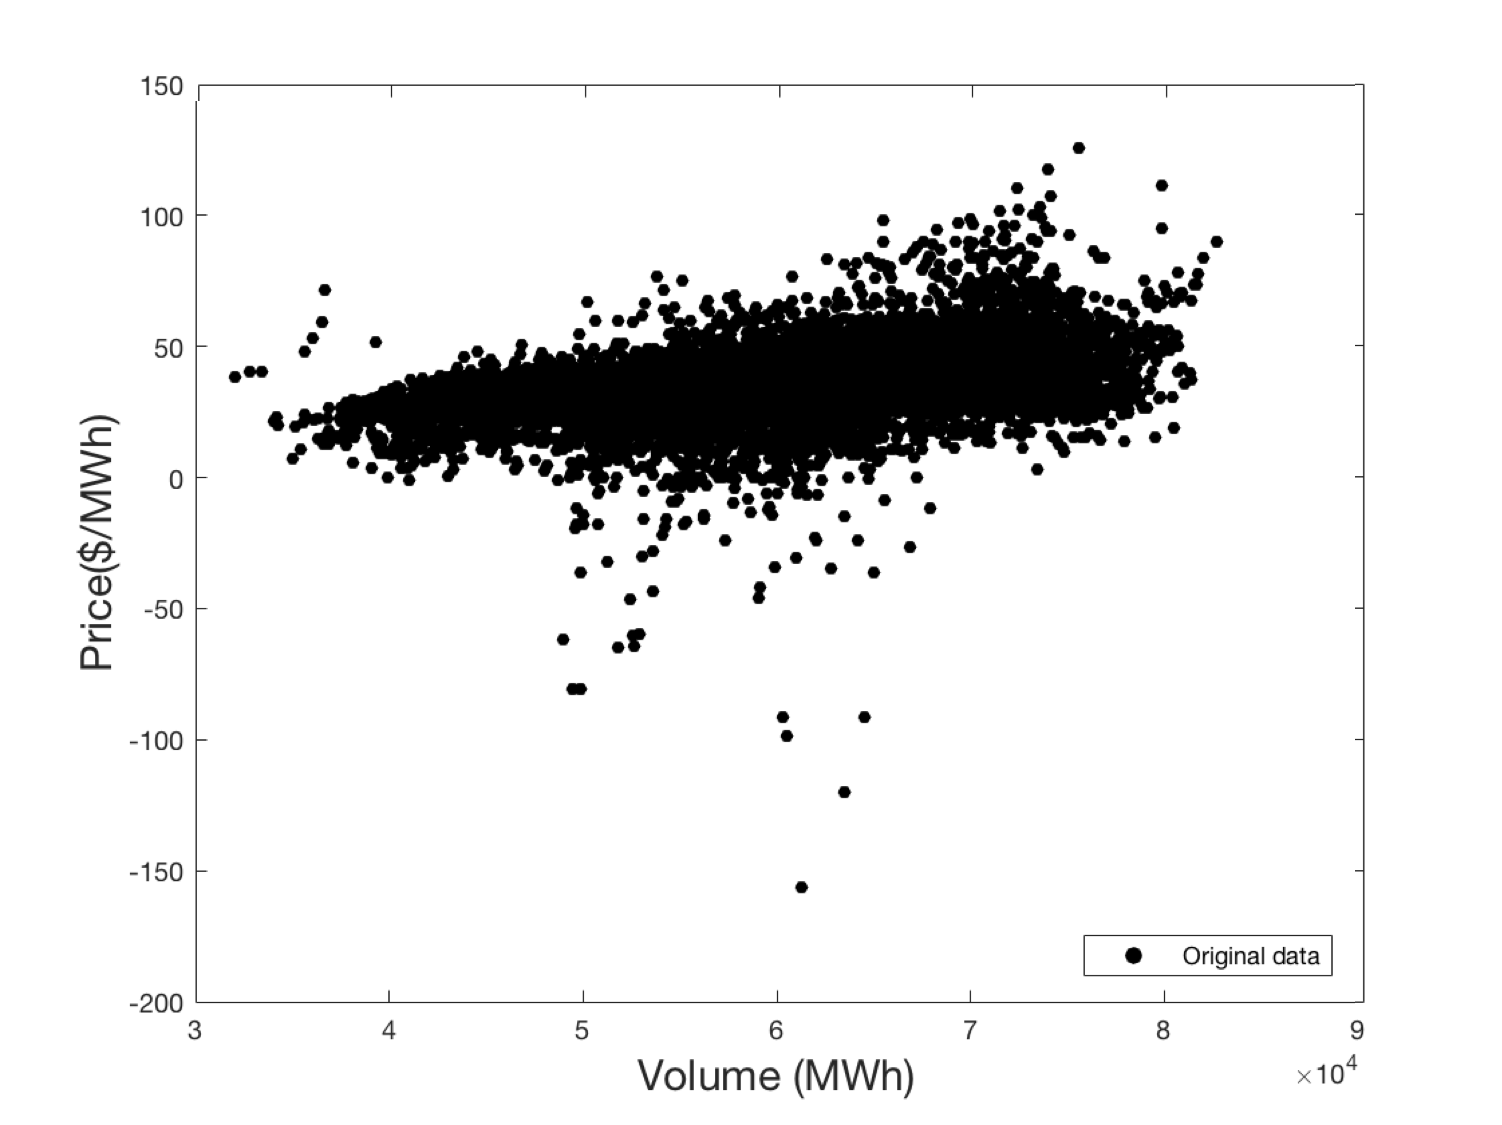
\includegraphics[width=0.95\linewidth]{Figures/Merit-order-original}
	\caption{Germany day-ahead price-volume data in 2016}
	\label{fig:merit-orignal}
\end{figure}

The pattern of merit-order effect is not clearly recognizable from the original data mainly due to the disturbs of variable renewable generation which has raised significantly in past years. This prevents us from directly applying merit-order models developed by previous studies\cite{He2013}\cite{Grunewald2012a}. Therefore, we applied the algorithm described in Section \ref{sec:market-simulation} which take into account the renewable generation and bounded flexibility of conventional generations. Figure \ref{fig:merit-transformed} shows the transformed pattern of data where a clearer merit-effect is identifiable. Figure \ref{fig:merit-classified} projects the classification to the original data distribution and it can be seen that the algorithm has successfully separated the data points where the price was driven to be higher or lower than average level due to the uplift effects introduced in \ref{sec:market-simulation}. 

\begin{figure}[h!]
	\centering
	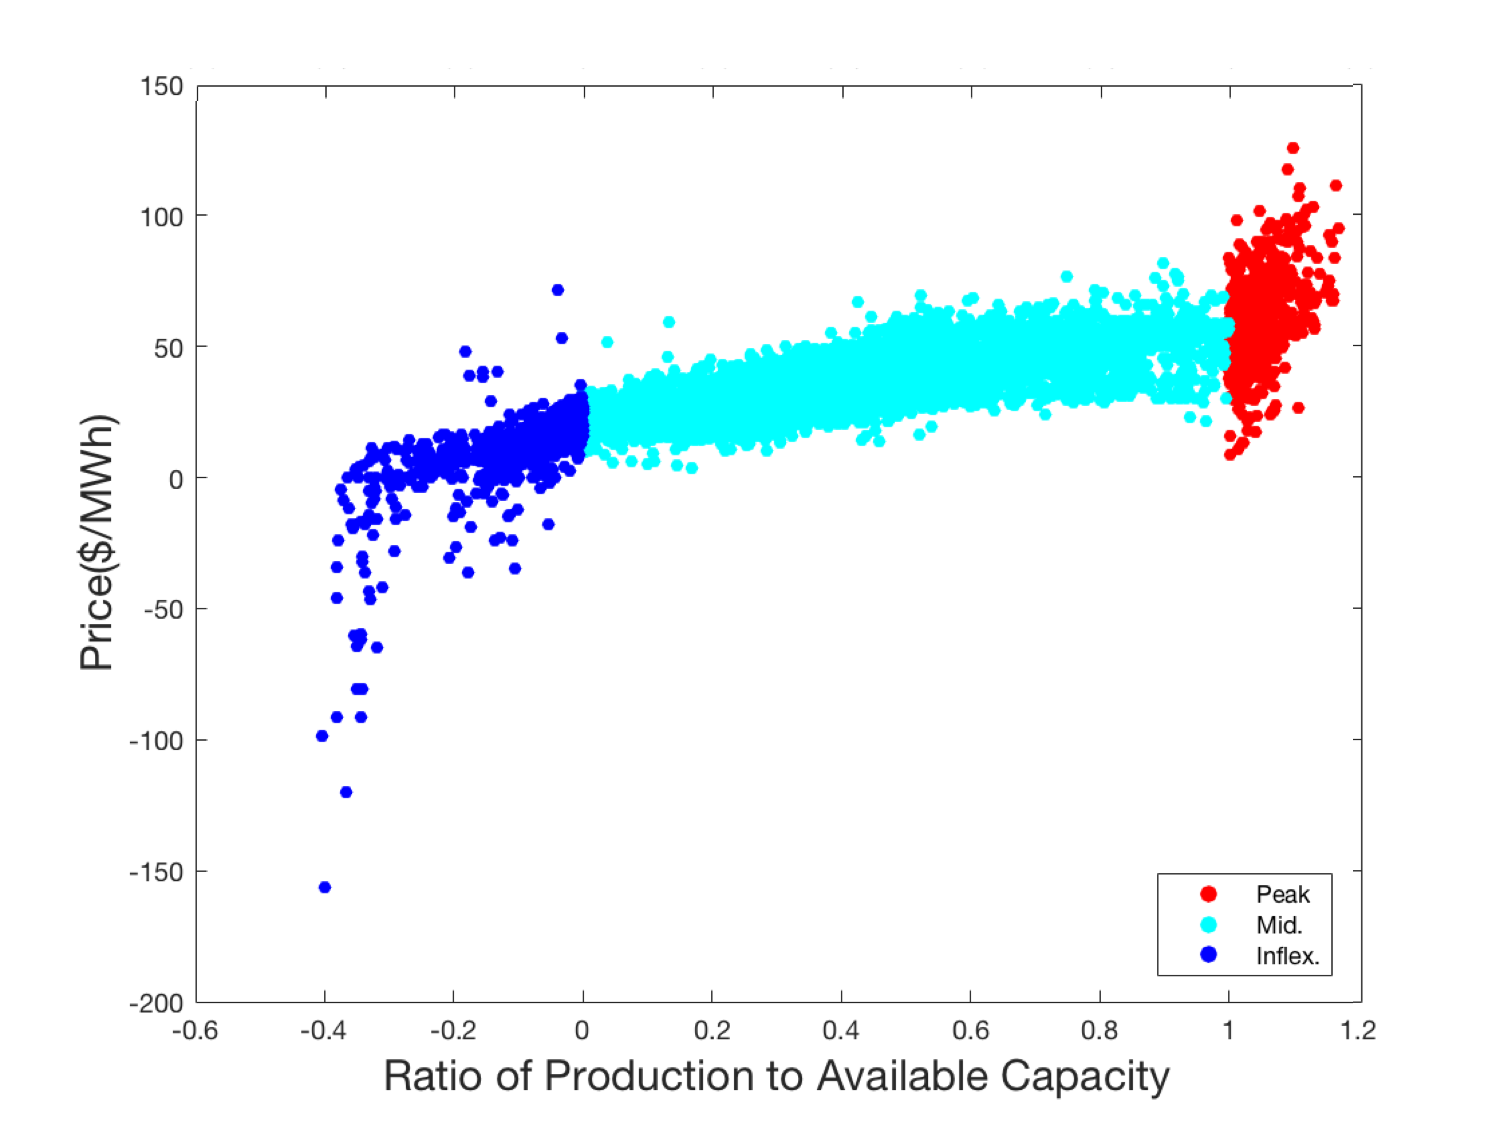
\includegraphics[width=0.95\linewidth]{Figures/Merit-order-transformed}
	\caption{Transformed pattern of Germany day-ahead price-volume data in 2016}
	\label{fig:merit-transformed}
\end{figure}
\begin{figure}[h!]
	\centering
	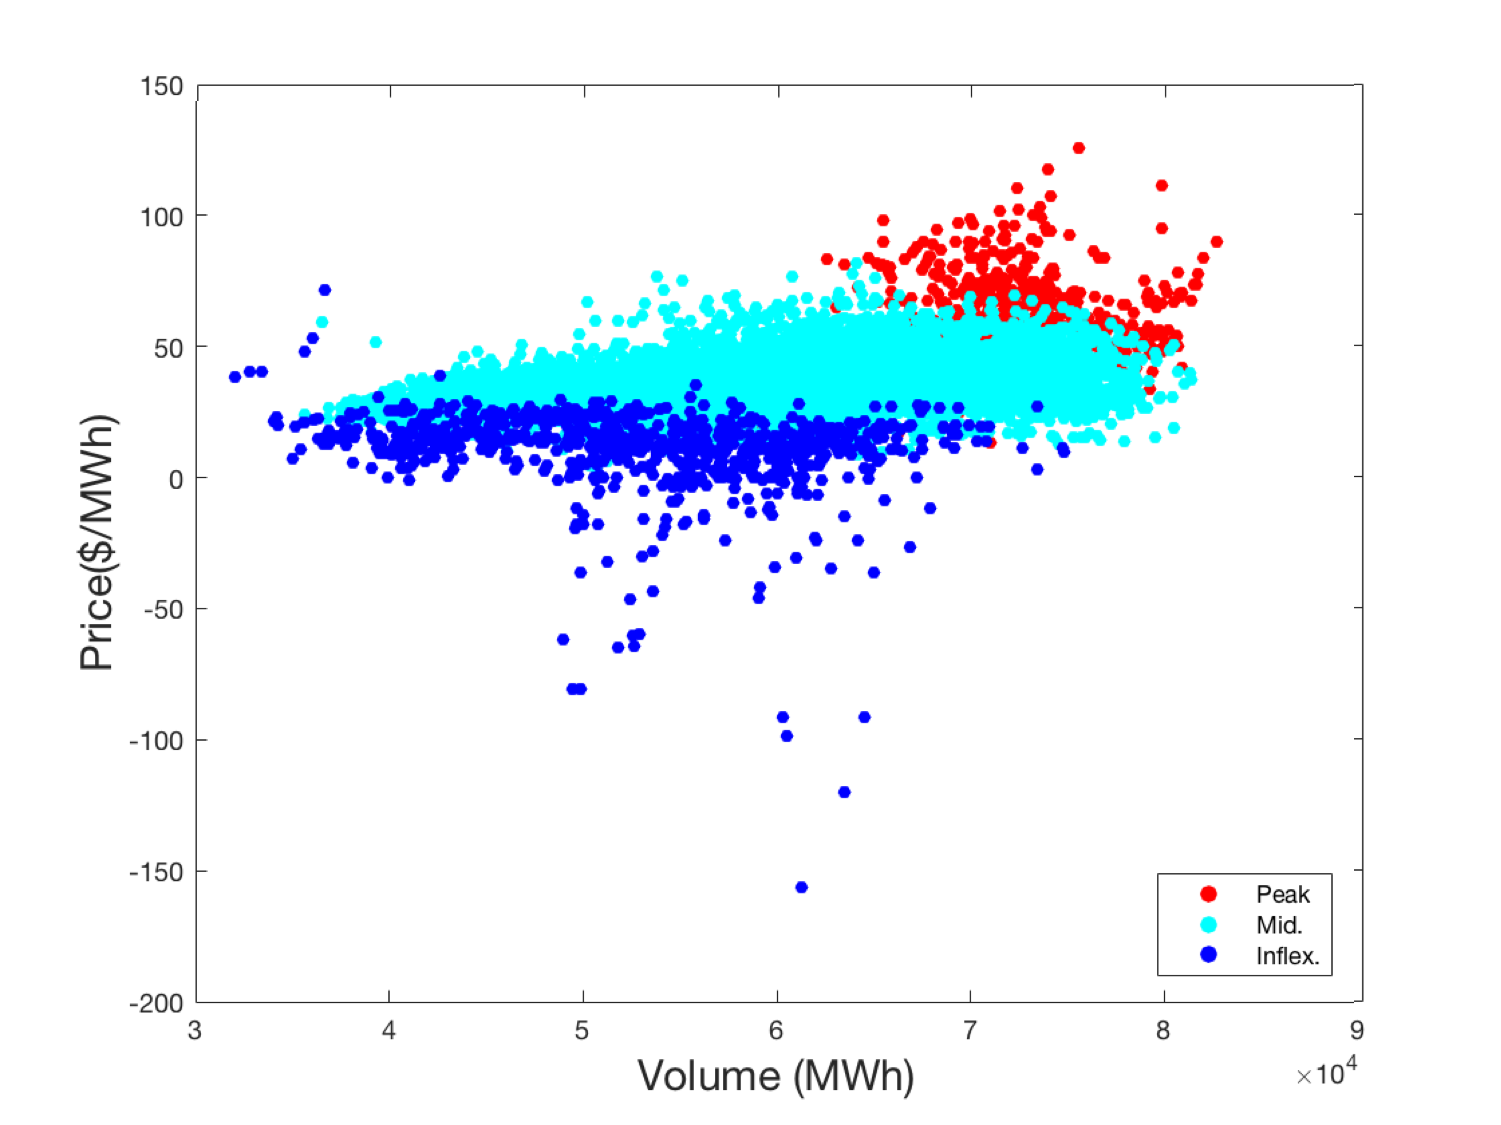
\includegraphics[width=0.95\linewidth]{Figures/Merit-order-classified}
	\caption{Classification of Germany day-ahead price-volume data in 2016}
	\label{fig:merit-classified}
\end{figure}

Thereafter, we fitted the transformed data pattern with the piece-wise function defined by \eqref{eq:merit-order-model}. The estimated parameters are listed in Table \ref{tab:merit}. It shall be noticed there are price limits applied in EPEX day-ahead market\cite{EPEX_price_limit} which is between -500 to 3000 EUR/MWh, equal to -600 to 3.6 USD/MWh using the specified currency exchange rate. The fitted merit-order curve is illustrated by Figure \ref{fig:merit-fitted} and distribution of errors between the fitted price and actual price is shown by Figure \ref{fig:merit-error}.

\begin{table}[h!]
	\centering
	\begin{tabular}{l  r r r}
		\hline
		\multirow{2}{*}{\textbf{Class}} & \multicolumn{3}{c}{\textbf{Parameters}}\\
		 & $a$ & $b$ & $c$\\
		\hline
		Inflex. & 17.05 & -1.49 & -12.35 \\
		\multirow{3}{*}{Mid.} & 48.66 & 16.40 & \\
		\multirow{3}{*}{} & 38.04 & 20.12 & \\
		\multirow{3}{*}{} & 16.37 & 34.20 & \\
		Peak & -194.95 & 491.46 & -0.69 \\
		\hline
	\end{tabular}
	\caption{Parameters of the merit-order model in Germany}\label{tab:merit}
\end{table}

\begin{figure}[h!]
	\centering
	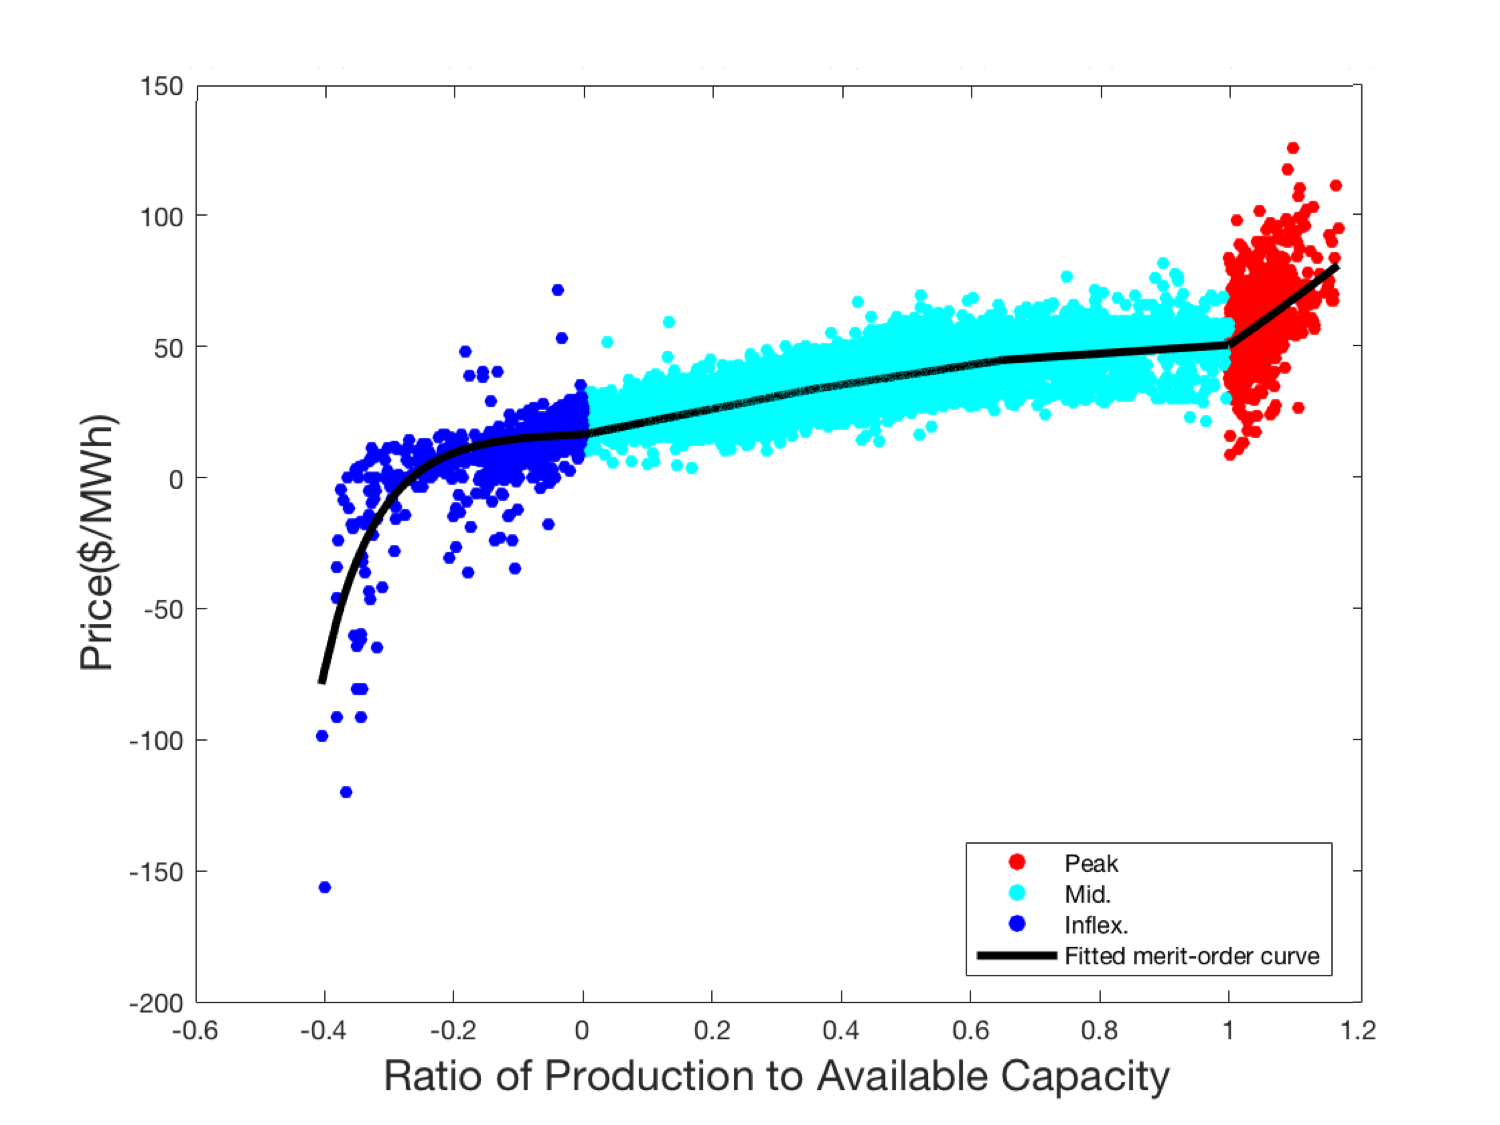
\includegraphics[width=0.95\linewidth]{Figures/Merit-order-fitted}
	\caption{Fitted merit-order curve with Germany day-ahead price-volume data in 2016}
	\label{fig:merit-fitted}
\end{figure}

\begin{figure}[h!]
	\centering
	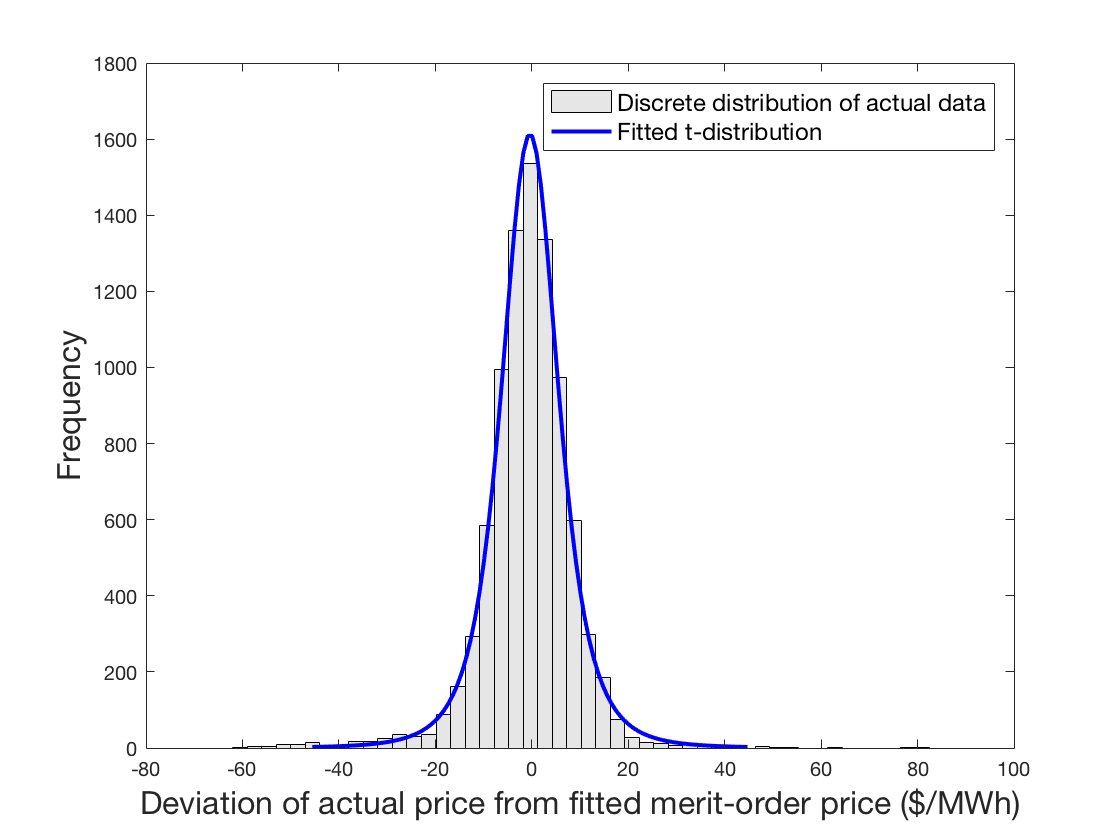
\includegraphics[width=0.9\linewidth]{Figures/4_Error-distribution}
	\caption{Distribution of errors between fitted merit-order price and actual price}
	\label{fig:merit-error}
\end{figure}

We simulated the day-ahead price using this merit-order model and compared to the actual market data. It can seen from Figure \ref{fig:merit-fitted}-\ref{fig:merit-error} that while the fitted merit-order price shows a good fitness to the actual price in terms of general trend, the stochastic movements of the price are eliminated. Merely with the merit-order model, a smoothed curve of price time-series would be generated where the drastic jumps of price cannot be captured, as is demonstrated by Figure \ref{fig:price-example}.

\begin{figure}[h!]
	\centering
	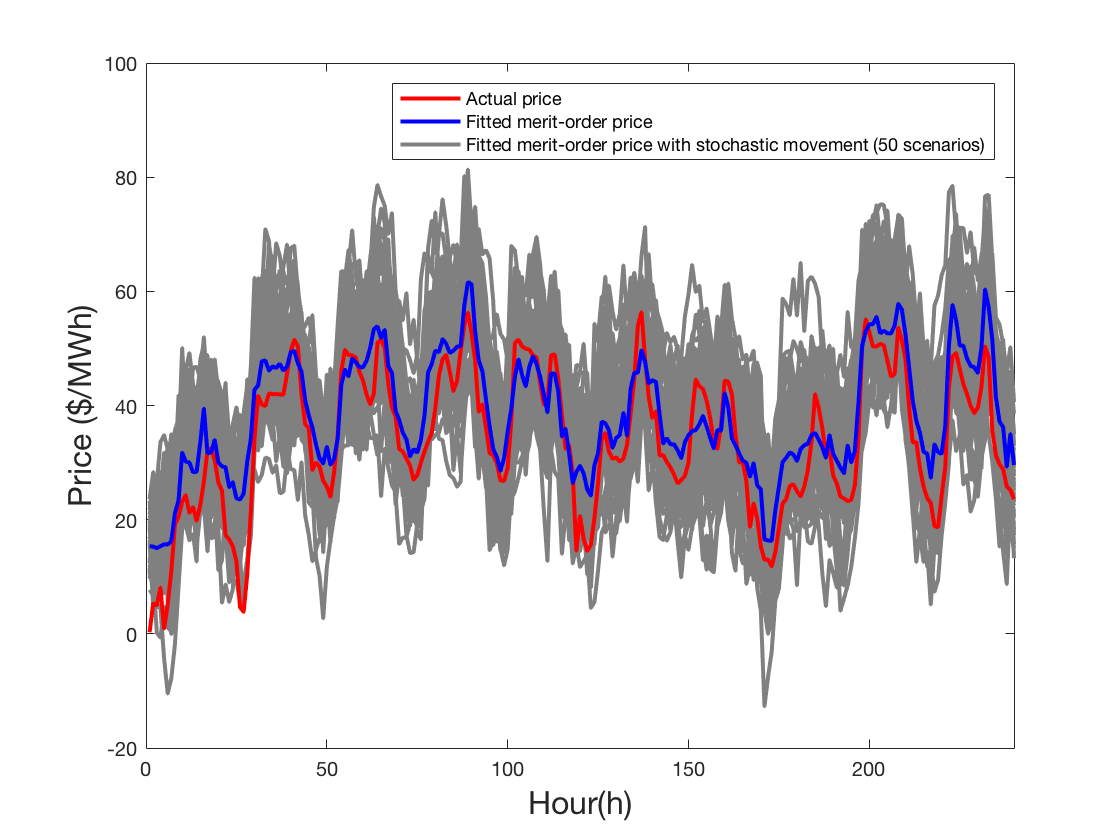
\includegraphics[width=0.95\linewidth]{Figures/5_Example-simulated_price}
	\caption{Generated price scenarios}
	\label{fig:price-example}
\end{figure}

Unlike studies on valuation of a conventional generation resources where such a merit-order model may suffice, the elimination of stochastic price movement would reduce the value of arbitrage greatly as is shown by Figure \ref{fig:model-validation}. This shall be understood intuitively as arbitrage activities pick the price differences among different trading slots and less volatile price movements would certainly affect the value creation of arbitrage.

\begin{figure}[h!]
	\centering
	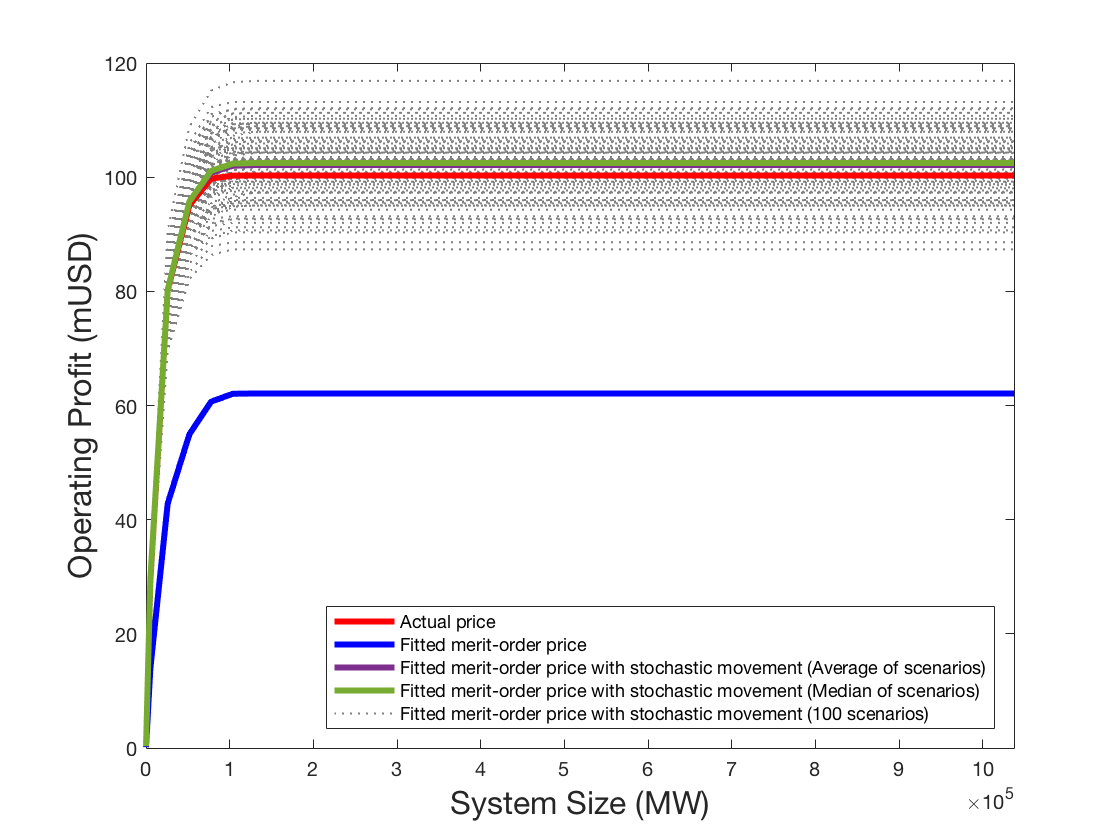
\includegraphics[width=0.95\linewidth]{Figures/6_Model_Validation}
	\caption{The revenue with different price scenarios for model validation in Germany}
	\label{fig:model-validation}
\end{figure}

\begin{table}[h!]
	\centering
	\begin{tabular}{r r}
		\hline
		\multicolumn{2}{c}{SARMA parameters}\\
		\hline
		$\phi_1 = 1.811$ & $\theta_1 = -1.063$ \\
		$\phi_2 = -0.813$ & $\theta_{24} =0.692$ \\
		$\phi_{24} = 0.090$ & $\theta_{168} = -0.600$ \\
		$\phi_{168} = 0.692$ & \\
		\hline
	\end{tabular}
	\caption{Parameters of the stochastic price movement of SARMA models in Germany}\label{tab:SARMA}
\end{table}

Therefore, a seasonal auto-regressed moving-average (SARMA) model as is described in \ref{sec:market-simulation} is applied to simulate the stochastic components of the price. The estimated parameters of the SARMA model based on the error signal characterized by\ref{fig:merit-error} is listed in Table \ref{tab:SARMA}. Thereafter, we conducted Monte-Carlo simulations and generated a number of scenarios of the stochastic parts of price which are then added to the determinate trends calculated by the merit-order model. The final simulated price scenarios are illustrated by the grey lines in Figure \ref{fig:price-example}. Using these generated price profiles, we calculated the revenue for 100 scenarios and compare the average and median value to the result obtained with actual price signal, which shew perfect fitness in Figure \ref{fig:model-validation}. There are no significant differences between the average and median value observed, but for robustness and avoiding effects of outliers, we would use the median value as the simulated result for experiments in proceeding sections.

We applied the same procedure to develop the model for PJM. It was noticed that the situation when the residual load is in the range of inflexible generation is rarely observed in PJM, which can be explained by the relative low installed capacity of renewable generations. Therefore, we migrated part of the merit-order model for inflexible generation based on Germany's data here, which shall however have insignificant effects because the lowest price is bounded at 0. Negative pricing is not explicitly an issue in PJM's market so far although PJM is fully aware of this issue but waiting for FERC's initiative to address the potential negative price formation\cite{PJM_price_limit_1}. Without unambiguous rules, we would not allow negative prices in our modeling. The highest price, on the other hand in PJM is capped at 1000 USD/MWh\cite{PJM_price_limit}. 

The parameters for the merit-order model in PJM are listed in Table \ref{tab:merit_pjm}. The SARMA parameters are presented in Table \ref{tab:SARMA_PJM}.

\begin{table}[h!]
	\centering
	\begin{tabular}{l  r r r}
		\hline
		\multirow{2}{*}{\textbf{Class}} & \multicolumn{3}{c}{\textbf{Parameters}}\\
		& $a$ & $b$ & $c$\\
		\hline
		Inflex. & 17.05 & -1.49 & -12.35 \\
		\multirow{3}{*}{Mid.} & 23.50 & 16.40 & \\
		\multirow{3}{*}{} & 32.02 & 13.41 & \\
		\multirow{3}{*}{} & 3.58 & 31.90 & \\
		Peak & 10.70 & 501.35 & -5.32 \\
		\hline
	\end{tabular}
	\caption{Parameters of the merit-order model in PJM}\label{tab:merit_pjm}
\end{table}

\begin{table}[h!]
	\centering
	\begin{tabular}{r r}
		\hline
		\multicolumn{2}{c}{SARMA parameters}\\
		\hline
		$\phi_1 = 0.690$ & $\theta_1 = 0.107$ \\
		$\phi_2 = 0.125$ & $\theta_{24} =-0.003$ \\
		$\phi_{24} = 0.298$ & $\theta_{168} = -0.399$ \\
		$\phi_{168} = 0.560$ & \\
		\hline
	\end{tabular}
	\caption{Parameters of the stochastic price movement of SARMA models in PJM}\label{tab:SARMA_PJM}
\end{table}


\subsubsection{Renewable penetration in Germany: at the inflection point}


\begin{figure}[h!]
	\centering
	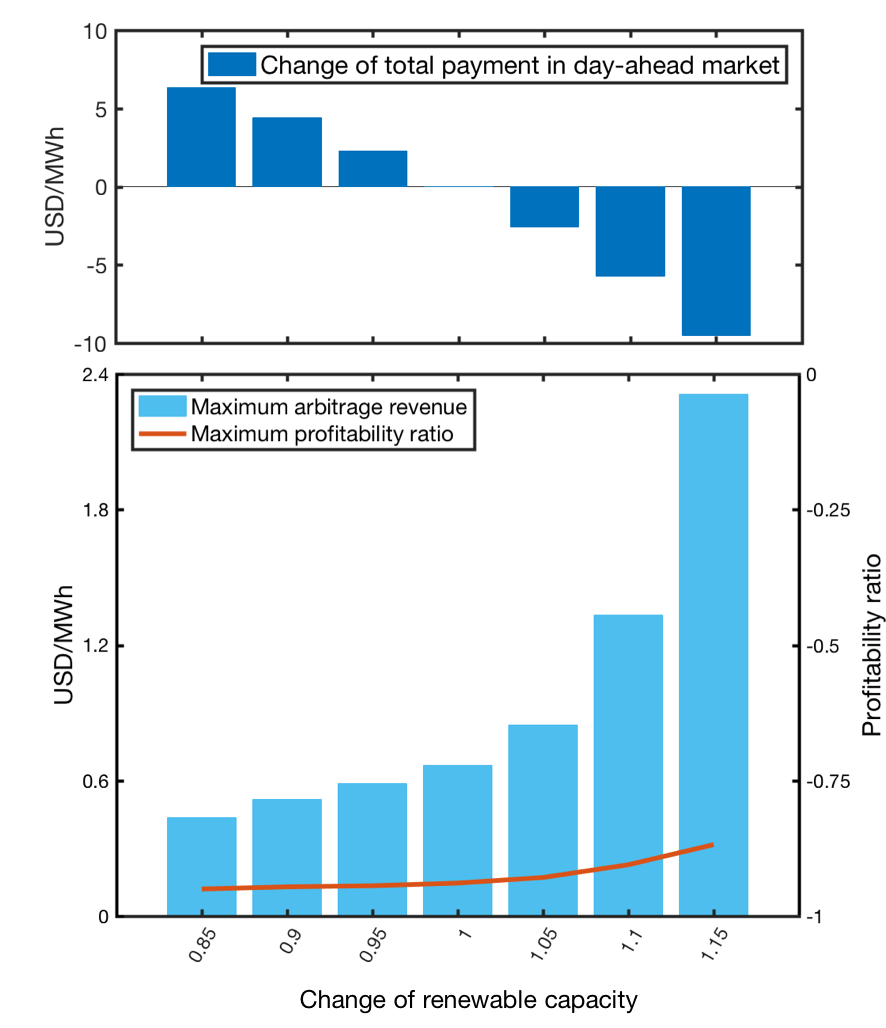
\includegraphics[width=0.95\linewidth]{Figures/RenewablePenetration_Germany}
	\caption{Impacts of renewable generations on revenue and profitability of arbitrage using flexibility as well as on total amount of transations in day-ahead market in Germany}
	\label{fig:renew_germany}
\end{figure}

The results are illustrated in Figure \ref{fig:renew_germany}. We can see while the revenue potential of arbitrage using flexibility grew insignificantly with renewable capacity growing from 85\% to the present level, it would accelerate rapidly afterwards. The potential revenue would almost double its value with 10\% additional renewable generation and triple with 15\% renewable growth. This indicates the day-ahead market in Germany is at a inflection point where the volatility will increase drastically with more renewable making it more favorable for arbitrage. Quantitatively, it was found when renewable capacity grew from 85\% to the present level, the addition of each 5\% growth would lead to a increase of 12-23\% on the
the standard deviation of day-ahead price. In contrast, the rises of volatility would be 74-225\% for each additional 5\% growth of renewable growth from present level to 115\%.

However, it is known that the renewable penetration will not only increase the price volatility but also lower the average level of price via the so-called merit-order effect. In our study, the merit-order effect was found to be 0.75 - 1.12 USD/MWh per additional GW of renewable generation, which accords with the number found by previous research where the merit-order effect was accounted to be 0.8-2.3 EUR/MWh  per additional GW in Germany by statistic studying on the real data between 2008 to 2012. 

Without any interventions, this effect would soon make the price unacceptably low to generators. In the scenario with 15\% more renewable the average price in day-ahead energy market will reduce by 14 USD/MWh which would almost half the revenues received by generators as a whole. The growth of arbitrage revenue would be one order of magnitude smaller than the reduction of overall amount of payment to generators. It was certain that players will take actions against this trend. The policy supports on renewables may also be gradually abated as what have already been noticed from the real world and introduced in Section \ref{sec:qualitative-analysis}. 

Market players with conventional generations that are suffering the pressure of decreasing price due to renewables may embrace flexibility in order to mitigate the conflicts of renewables and inflexible generations or even enhance their market power to strategically maintain the price level as is studied in \cite{Schill2011}. The effects of arbitrage using flexibility on wholesale energy market would be briefly discussed in Section \ref{sec:sensitivity} on a schematic level.

Nevertheless, BESS might not be the right choice to achieve these goals. As the profitability ratios of the pre-defined BESS in our study were still deeply negative and raised insignificantly to be optimally -87\% from nowadays's level of -94\%.

\subsubsection{Renewable penetration: arbitrage potential bounded by non-negative pricing}

Similar work was conducted in PJM's day-ahead market. Results are shown by Figure \ref{fig:renew_pjm}. With trivial addition of renewable generations from 85-115\%, the potential arbitrage revenue would increase slightly by about 0.7-1\% for each 5\% increment. However, further growth of renewables will lead to a decreasing trend of arbitrage potential. This could be explained because of the non-negative price. Without compensation from negative prices, the arbitrage value dropped along with the shrink of average electricity price due to merit-order effects. The merit-order effect here was found to be 1.05 - 1.13 USD/MWh per additional GW of renewable capacity.

\begin{figure}[h!]
	\centering
	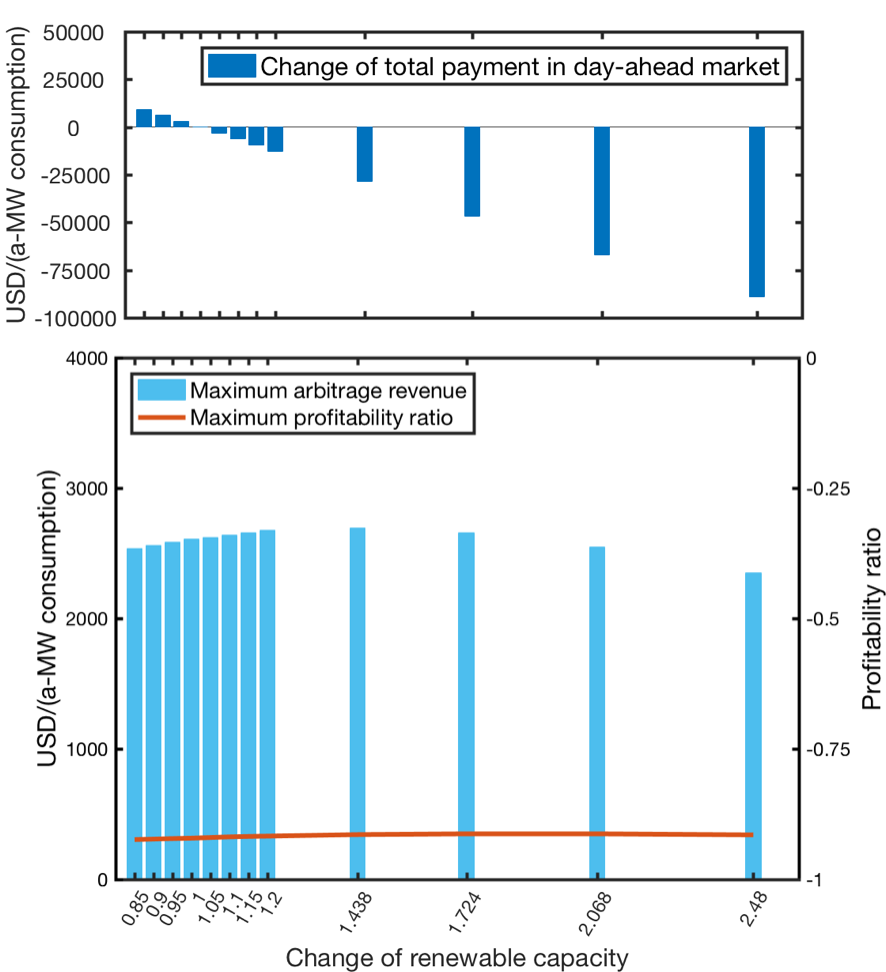
\includegraphics[width=0.95\linewidth]{Figures/RenewablePenetration_PJM}
	\caption{Impacts of renewable generations on revenue and profitability of arbitrage using flexibility as well as on total amount of transations in day-ahead market in PJM}
	\label{fig:renew_pjm}
\end{figure}

PJM reported that it had received negative offers from wind generation enabled by the federal wind production tax credit (PTC)\cite{PJM_price_limit_1}. However, without a clear framework of negative price formation, predictive studies would hardly be robust. 

\subsection{Sensitivity analysis}
\label{sec:sensitivity}
Throughout the whole study, there are two most important assumption made, i.e. the perfect predictability assumption and fixed price assumption. Elaborated in the literature, this two assumption are common pragmatic tools in similar studies to indicate a idealistic value as upper bound. 

\subsubsection{Limited predictability}


\subsubsection{Responsive price}

\subsubsection{Sensitivity analysis of other parameters}







\appendix

\chapter{Excess Data}
\lipsum[1-3]

\backmatter

\chapter*{Bibliography}
\chaptermark{Bibliography}
\addcontentsline{toc}{chapter}{Bibliography}
Put your references here.
\lipsum[1-5]

\end{document}
